% Header mit Deklarationen
\input{Sonderseiten/header.tex}
% Literaturverzeichnis
\bibliography{literatur/bib}

\begin{document}

% Römische Nummerierung für Sonderseiten, wie Verzeichnisse und Anhang
\pagenumbering{Roman}

% Titelblatt
\begin{titlepage}
\setcounter{page}{1}
%\thispagestyle {empty}
%\fancypagestyle{plain}{}
\begin{center}
%\vspace{2cm}
%\setlength{\headheight}{15pt}
\begin{figure}[h!]
\vspace{0cm}
\centering
% \includegraphics[width=0.6\textwidth]{graphics/HM_Deu_CMYK}
\includegraphics[width=0.8\textwidth]{bilder/Logos/FK03_CMYK_Block.png}
\\[0.8cm]
% \includegraphics[width=0.25\textwidth]{bilder/}
\end{figure}
\vspace{1.5cm}

{\fontsize{20}{60}\scshape Diplomarbeit} 
\\[1.1cm]

\begin{doublespace}
{\fontsize{30}{22}\selectfont \textbf{Konzeptionierung, Entwicklung und Erprobung der Bordelektronik eines unbemannten Kleinstflugzeuges}\par} 
\vspace{1.4cm}
\end{doublespace}

\title{Konzeptionierung, Entwicklung und Erprobung der Bordelektronik eines Unbemannten Kleinstflugzeuges}
\author{Jens Schmelkus}
\date{Dezember 2017}

{\fontsize{23}{60}\scshape Jens Schmelkus} 
\\[2.0cm]


\textbf{Betreuer}: Prof. Dr. Karl Siebold



% \textbf{Fakultät}: Fakultät für Maschinenbau, Fahrzeugtechnik, Flugzeugtechnik

\textbf{Studiengang}: Fahrzeugtechnik 

\textbf{Abgabe}: 22.01.2018

\vfill

% \colorbox{orange}{Name oben drüber Betreuer kleiner als meiner, Fakultät, keine Tabellenform, Diplomarbeit kleiner}

\end{center}
\end{titlepage}


\cleardoublepage\thispagestyle{empty}

\input{Sonderseiten/Eigenstaendigkeitserklauerung}


\cleardoublepage

% \input{Sonderseiten/Sperrvermerk}

\clearpage

\chapter*{Zusammenfassung}\addcontentsline{toc}{chapter}{Zusammenfassung}

Das Labor für systemtechnik Entwickelt, Produziert und betreibt seit 2010 im Rahmen sowohl von Studentischen als auch Forschungsprojekten verschiede Unbemannte Flugsysteme.
Der Schwerpunkt liegt hier bei Automatisch gesteuerten Flächenflugzeugen.
Das Abfluggewicht liegt zwischen 2 und 15 kg ,sowie Spannweiten wzischen 1,5 m und 5 m.

-->> Hier kurze erwähnung AUVSI 

-->> Komplexes System genötigt cverschiedenste Elektronik für Antrieb Aktuierung/Lenkung Funkkontakt Energiemenagement etc.

-->> Dafür wird in dieser Arbeit ein Elektrisches Funktionskonzept erstellt und die anforderungen Formuliert

-->> ES werden Baugruppen Entwickelt die die jeweiligen subanforderunge erfüllen sollen

-->> Test von subkompanenten (Ideale Diode)

-->> Elektronischer Gesamtaufbau entsteht und wird erklöärt

-->> Elektronikerprobung wird beschrieben und Messdaten fezeigt (so.)

-->> Flugversuch Praxistest ---> Wettbewerbseinsatz und Wettbewerbsergebnis

\begin{comment}

Die Firma Bihler entwickelt und produziert für ihre Stanz-Biegeautomaten NC-Aggregate. Mit diesen werden Werkzeuge präzise bedient, um Bauteile und Baugruppen in der Massenproduktion zu fertigen. Um zu vermeiden, dass es zu Funktionsfehlern bei den in Serie gefertigten NCAs kommt, wird durch Prüfen während des Produktionsprozesses versucht, derartige Probleme so weit wie möglich zu auszuschließen. Obwohl die Aggregate bereits ein Prüfverfahren durchlaufen, werden nicht alle gravierenden Fehler entdeckt. Deshalb wird das derzeitige Prüfen analysiert und es werden Vorschläge zu einer eventuell nötigen Überarbeitung entwickelt.


Hierzu wird der Aufbau der verschiedenen Varianten der NCAs dargestellt, die elektronische Ansteuerung unter Zuhilfenahme des Kurvengetriebes erläutert und die Fahrbewegung der NCAs im Trapez- und Dreiecksprofil aufgezeigt. Es wird festgestellt, dass Funktionsstörungen der NCAs die verschiedensten Ursachen haben und alle am Produktionsprozess Beteiligten damit konfrontiert sind.

Der derzeitige Testlauf auf einem Prüfstand integriert das Einlaufen der Aggregate und erfasst beim kompletten Ein- und Ausfahren der Pinole während eines bestimmten Testzyklus im Bewegungsprofil Trapez Stromstärke und verschiedene Temperaturwerte. Hierdurch können Fehler aber nicht zuverlässig aufgedeckt werden, zumal keine Standards für die funktionsspezifischen Eigenschaften der NCA vorhanden sind und es kein Dokumentationssystem zur Erfassung von Problemen und deren Rückmeldung an die entsprechenden Abteilungen gibt.


Nach einer Auseinandersetzung mit den Grundlagen von Prüfkonzepten und Testverfahren werden deshalb teilweise auf der Grundlage des bisherigen Testablaufs entwickelte Testverfahren geprüft und bewertet. Dabei darf bei allen Testkonzepten der ökonomische Aspekt nicht außer Acht gelassen werden.

Das bisher schon eingesetzte langsame Abfahren im Trapezprofil ist wenig geeignet, da die Einflüsse des Reglers nicht erkennen lassen, ob eine Schwergängigkeit vorliegt. 

Aufgrund der Versuche kann davon ausgegangen werden, dass man weitreichende Erkenntnisse zu etwaigen Störungen durch das Belasten der NCAs beim Betreiben erhält. Da sich Tests mit einem direkten Belasten der Achse durch Anhängen einer Last oder Fahren auf einen Widerstand nicht als praxistauglich erweisen, werden Messungen analysiert, die aufgrund des Fahrprofils die Achsen dynamisch belasten. 

So wird das Fahrprofil Polynom 5. Ordnung neu entwickelt und berechnet. 19 NCAs werden mit dem Fahrprofil Polynom 5. Ordnung und mit dem Fahrprofil Stufenprofil gemessen und daraus Mittelwertkuren und Standardabweichungen berechnet. Bei einer Achse wird hierbei axiales Spiel hoch signifikant erkannt. Es bietet sich an, die Verfahrprofile Stufenprofil und Polynom 5. Ordnung einzusetzen, denn mit ihnen können die Achsen bis an die Belastungsgrenzen belastet werden und es lässt sich axiales Spiel erkennen. Weiterhin lassen sich diese Messungen leicht in den vorhandenen Prüfablauf integrieren.



Voraussetzung ist, dass auf eine für das Steuern der Achsen in Tests geeignete Steuerung zurückgegriffen werden kann, die auch das Aufzeichnen und Analysieren von Daten unterstützt. Dies ist mit der derzeitigen, nicht für den Testbetrieb ausgelegten VC 1 Steuerung nur sehr eingeschränkt möglich.

Als weitere Testmöglichkeit werden Schwingungsmessungen untersucht. Hierbei werden zuerst die zu erwartenden Schwingungsfrequenzen berechnet. Anschließend werden Versuche durchgeführt, um die grundsätzliche Eignung von Schwingungsmessungen als geeignete Messmethode zu evaluieren. Eine Analyse der Versuchsergebnisse zeigt, dass Schwingungsmessungen dazu geeignet sind, um Funktionsstörungen an den NCAs zu erkennen. Jedoch müssen weiterführende Versuche durchgeführt werden, um standardisierte Tests zu entwickeln.

Mit der Erfassung von Temperaturwerten wie Motortemperatur oder der Temperatur an den NCAs mithilfe externer Sensoren könnten zwar aussagefähige Ergebnisse gewonnen werden. Jedoch ist die Entwicklung praxistauglicher Messverfahren sehr aufwendig und bringt im Vergleich zu den anderen als geeignet erscheinenden Messverfahren keine entscheidenden Vorteile.


%Die Messung von Temperaturwerten wie Motortemperatur oder die Temperaturmessung mithilfe von externen Sensoren an den NCA ist im Vergleich zu den anderen untersuchten Messmethoden schwierig in der Umsetzung zu aussagekräftigen Messverfahren.





%Zudem haben Volumenstromessungen am Kühlmittel ergeben, dass man auch diese Messungen zur Analyse des Kühlsystems heranziehen kann.

Zur Analyse des Kühlmitteldurchflusses innerhalb des Aggregats wird ein Kennwert entwickelt. Aus der  Messung mehrerer Aggregate wird wiederum ein Mittelwert und dessen Standardabweichung abgeleitet,  die für das Testen zur Verfügung stehen.

Die Ergebnisse der Arbeit schaffen die Grundlage, an Hand derer das Prüfverfahren überarbeitet werden kann.



\end{comment}


\clearpage

% Verzeichnisse
% Kopfzeile links Kapitel, rechts leer
%\ihead{\leftmark}
%\ohead{}
%\input{Sonderseiten/verzeichnisse}

%
% Inhaltsverzeichnis
%
\tableofcontents \addcontentsline{toc}{chapter}{Inhaltsverzeichnis}%\pdfbookmark[0]{Inhaltsverzeichnis}{sumario_label_pdf}


\input{Sonderseiten/nomenklatur}


%
% Abkürzungsverzeichnis
%
\input{Sonderseiten/abkuerzungen}
\printglossary[title={Abkürzungsverzeichnis},toctitle={Abkürzungsverzeichnis},type=\acronymtype,style=long]








% Merke mir die römische Seitenzahl in 'roemisch' und setzte Nummeriernung 

% auf arabisch für die eigentlichen Kapitel
\cleardoublepage

\newcounter{roemisch}
\setcounter{roemisch}{\value{page}}
\pagenumbering{arabic}

%\begin{comment}
%\input{kapitel/Einleitung}

\cleardoublepage

%\chapter{Einleitung}


\section{Motivation}

Die Otto Bihler Maschinenfabrik GmbH \& Co. KG ist ein Systemlieferant in der Stanzbiege"~, Schweiß- und Montagetechnik. Seit 60 Jahren setzt sich die Firma mit zukunftsweisenden Fertigungssystemen und -lösungen auseinander. Es handelt sich um  ein mittelständisches Unternehmen mit weltweit etwa 900 Beschäftigten. Außer am Hauptsitz in Halblech im Allgäu wird an zwei weiteren Standorten, in Füssen im Allgäu und in den USA (Phillipsburg, New Jersey), produziert. 

Die 1953 von dem Flugzeugmechaniker Otto Bihler eröffnete Werkstatt zur Fertigung von Federn mündete über die Entwicklung der ersten radialen Draht- und Bandbiegeautomaten 1958 in die Gründung der Otto Bihler Maschinenfabrik KG. 

Bei der Stanz-Biege-Technik handelt es sich um ein trennendes und umformendes Fertigungsverfahren, bei dem ein oder mehrere Halbzeuge, wie z.B. Metallbänder oder Metalldrähte, auf einem einzigen Automaten, der Stanz-Biege-Maschine, zu einem fertigen Produkt verarbeitet werden. \cite{Hoermann2013}

Da den Stanz-Biege-Maschinen seit 1966 ein Baukastensystem zugrunde liegt, besitzen sie eine Vielzahl an Bearbeitungsvariationen und Umformmöglichkeiten und es wurden immer weitere Prozessschritte in das Bearbeitungssystem integriert. Neben den Stanz-Biege-Maschinen, die das Kerngeschäft der Firma Bihler bilden, werden deshalb die Montagemaschinen immer wichtiger. Auf ihnen können in Kombination mit Stanz-Biege-Maschinen unter dem Einsatz von weiteren Bearbeitungsschritten, wie Montieren, Schweißen, Gewindeschneiden, Messen, Verpacken und Beschriften, ganze Herstellungsprozesse realisiert werden. Es eröffnen sich Möglichkeiten zu einer Komplettfertigung von immer komplexeren Bauteilen und Baugruppen  bei minimalem Material- und Energieeinsatz, was den Anforderungen der Zulieferindustrie entgegenkommt.

Die Bihler Technologie wird in verschiedensten Industriezweigen eingesetzt. So findet man die Maschinen und die darauf produzierten Produkte laut \cite{Hoermann2013} in der Automobilindustrie, Elekto- und Elektronikindustrie, Medizintechnik, Registratur- und Verbindungstechnik, Schmuckindustrie, Federn- und Drahtindustrie, Kommunikationstechnik, Eisen-, Blech- und Metallwarenindustrie sowie der Umwelttechnik.


Historisch erfolgte der Antrieb in den meisten Maschinentypen über ein von einem Elektromotor angetriebenens Großrad. Die auf der Maschine eingesetzten Aggregate werden entweder direkt oder über eine Übersetzung durch das Großrad angetrieben. Durch diese zwangsangetriebenen Aggregate können alle Bearbeitungsschritte ohne zusätzliche Steuerung realisiert werden. Nachteilig ist hier, dass Bewegungen, die nicht innerhalb einer Maschinenumdrehung durchgeführt werden können, aufwendig durch \gls{NC}-gesteuerte Hilfsaggregate oder durch Pneumatik ausgeführt werden müssen.

Die Steuerung der mechanischen Maschinen erfolgt über Kurvenscheiben. Hierbei wird die rotatorische Bewegung des Großrades auf das Aggregat übertragen und über die Kurvenscheiben in eine Linearbewegung umgewandelt. Kurvengetriebe sind sehr kompakt und zuverlässig und ermöglichen einen schnellen Werkzeugwechsel, da nur die Kurvenscheibe ausgetauscht werden muss. Dennoch sind sie bei den immer kleiner werdenden Losgrößen heutzutage nicht flexibel genug, um schnell und kostengünstig zu produzieren.

Schon im Jahr 2000 wurde das erste komplett elektronisch gesteuerte \gls{CNC}-Umformsystem entwickelt. So wurden unter anderem die mechanisch angetriebenen Schlittenaggregate durch elektrisch direkt angetriebene und elektronisch gesteuerte \glspl{NCA} (NCAs) ersetzt. Der Durchbruch auf dem Markt gelang der NC-Technik im Hause Bihler mit den sehr flexiblen BIMERIC Maschinen. Diese sind durch das Baukastensystem besonders gut für Montageaufgaben geeignet. Mit den neu entwickelten GRM-NC und RM-NC Maschinen stehen Aggregate zur Verfügung, die die klassisch mechanisch gesteuerten Stanz-Biege-Automaten ersetzen können. 


Eines der Hauptelemente der NC gesteuerten Maschinen sind hierbei die Numerical Controlled Aggregate (NCAs). Diese ersetzen die kurvengesteuerten Aggregate und sind für die Ausführung von Werkzeugbewegungen verantwortlich. Die benötigte Stückzahl an NCAs ist in den letzten Jahren stark gestiegen, da sie sich als für den Kunden vorteilhaft in der Produktion von komplexen Bauteilen herausgestellt haben. Die Anforderungen an die NCAs im Einsatz sind sehr hoch, da sie ständig und mit hoher Belastung laufen müssen. Zudem handelt es sich bei den NCAs um eine für den Stanz-Biegebereich neue Technologie, die sich in der Weiterentwicklungs- und Optimierungsphase befindet.




Der Einsatz der NCA Technologie im Hause Bihler geht auf die Konstruktion und Entwicklung dieser Aggregate im eigenen Haus zurück. Es werden Prototypen gebaut, getestet und weiterentwickelt. Die NCAs werden inzwischen in Serie am Standort Füssen gefertigt und montiert. Für die verschiedenen Einsatzzwecke gibt es verschiedene Varianten, die sich im Verfahrweg, der Verfahrgeschwindigkeit, den Kräften und daraus bedingt in der Größe und dem Gewicht unterscheiden.

Um den hohen Qualitätsansprüchen der Firma Bihler gerecht zu werden, werden die NCAs, nachdem sie fertig montiert sind, im Werk einem Testlauf unterzogen. Neben dem eigentlichen Testen dient der Testlauf auch dazu, die Aggregate einlaufen zu lassen. Nach dem Testlauf werden die NCAs direkt in neue Maschinen verbaut oder als Ersatzgeräte an Kunden ausgeliefert. Jedoch treten bei Kunden immer wieder Fehler auf, so dass die schadhaften NCAs zurückgeliefert und durch die Firma Bihler repariert bzw. ersetzt werden müssen.


\section{Aufgabenstellung}

Dies ist der konkrete Anlass dafür, sich mit dem Testablauf der NCAs auseinanderzusetzen. Denn einwandfrei funktionierende NCAs sind grundlegend für die Produktion beim Kunden und es kann bei ihm zum Stillstand der Maschine und dadurch bedingt einem erheblichen Produktionsausfall kommen, wenn sie fehlerhaft sind. Deshalb müssen durch das Testen vor dem Einbau in eine Maschine möglichst weitgehend alle möglichen Fehlerquellen ausgeschlossen werden. Bei vom Kunden zurückgelieferten Aggregaten wurde zum Beispiel Spiel festgestellt. Dieses Spiel ist durch den bisherigen Testlauf nicht erkannt worden.



% Konkrete Anlässe dafür, sich mit dem Testablauf auseinanderzusetzen, ergeben sich daraus, dass bei den Kunden Fehler auftreten und die schadhaften NCAs zurückgeliefert und durch die Firma Bihler repariert bzw. ersetzt werden müssen. Da  einwandfrei funktionierende NCAs grundlegend für die Produktion beim Kunden sind und es bei ihm zum Stillstand der Maschine und dadurch bedingt einem erheblichen Produktionsausfall kommen kann, wenn sie fehlerhaft sind, müssen durch das Testen vor dem Einbau in die Maschine möglichst weitgehend alle möglichen Fehlerquellen ausgeschlossen werden. Bei vom Kunden zurückgelieferten Aggregaten wurde zum Beispiel Spiel festgestellt. Dieses Spiel ist durch den bisherigen Testlauf nicht erkannt worden.

So ist der derzeitige Testablauf nach Ansicht der Firma Bihler nicht optimal gestaltet und es ist Aufgabe dieser Diplomarbeit, den Prüfprozess der NCAs in der Serienfertigung zu analysieren und gegebenfalls zu überarbeiten. Falls nötig, sollen neue Prüfkriterien bzw. Testmerkmale gefunden und Testmöglichkeiten entwickelt werden. 

Die Arbeit wird in der Abteilung Serienbetreuung der Firma Bihler am Standort Füssen durchgeführt. Dort können sowohl die Erfassung und Auswertung des derzeitigen Testablaufs, als auch das theoretische Erarbeiten  möglicher Testmodelle sowie das Testen verschiedener NCAs mit verschiedenen Testmodellen am bereits vorhandenen Prüfstand der NCAs vorgenommen werden.


In dieser Arbeit wird schwerpunktmäßig mit den konkreten Werten eines bestimmten NCA-Typs, mit der Artikelnummer 100-54-0700.5 (NCA 4 / 120.19000 P=10 vgl. \cite{Riedle2015}), gerechnet. Die hier dargestellten Methoden sind jedoch für alle NCAs gültig. Auf mögliche Unterschiede und Probleme wird in den einzelnen Kapiteln eingegangen. Aufgrund der Größe und des Handlings sind die Varianten der NCA7 kein Bestandteil dieser Arbeit.










\cleardoublepage

%\chapter{NC-Aggregate}



NCAs sind seit einigen Jahren ein neu hinzugekommener, selbst entwickelter Teil des Bihler Baukastensystems zur Massenfertigung von Präzisionsteilen auf deren Stanz-, Biege- und Umformautomaten. \cite{OttoBihlerMaschinenfabrikGmbH&Co.KG2012} Innerhalb dieses Systems dienen sie dazu, Werkzeugbewegungen schnell und exakt auszuführen, d.h. sie stellen hohe Kräfte und schnelle Bewegungen bereit.



Parallel dazu werden auf anderen Maschinen auch noch die in früheren Jahren entwickelten über Kurvenscheiben gesteuerten Schlittenaggregate verwendet. Diese rein mechanisch gesteuerten Maschinen sind sehr robust und zuverlässig. Auch können mit ihnen sehr hohe Produktionsgeschwindigkeiten erreicht werden. Ihre Stärke liegt in der Produktion hoher Losgrößen, wo beständig große Mengen gleicher Teile hergestellt werden sollen. Die Rüstzeiten bei einem Werkzeugwechsel sind dagegen lang und wenn es, wie zumeist von der heutigen Wirtschaft gefordert, darum geht, die Lagerbestände gering zu halten und die entsprechenden Teile zum geforderten Termin zu liefern, dann haben die NC-Systeme entscheidende Vorteile.


Aus der Kombination von Mechanik, Elektrotechnik und Informatik ergeben sich für die NCAs im Vergleich zu den klassischen mechanisch angetriebenen Schlittenaggregaten folgende Vorteile: \cite{OttoBihlerMaschinenfabrikGmbH&Co.KG2012} 

\begin{itemize}
 \item Der Wechsel von mechanischen Komponenten beim Rüsten wird deutlich reduziert.
 \item Die Rüstzeit ist sehr kurz.
  \item Verschiedene Prozesse können schnell und einfach reproduziert werden. 
 \item Verschiedenste Prozesse können auf einer Anlage kombiniert und integriert werden.
 \item Hubbewegungen und Bewegungsprofile sind frei programmierbar.
 \item Der Umgang mit dem Werkstoff ist wegen der freien Programmierbarkeit der Fahrprofile sehr schonend.
 \item Die Maximalkraft ist über den gesamten Arbeitsbereich frei wählbar.
 \item Eine Kraftsteuerung ist möglich.
\end{itemize}






Insbesondere mit der neuen Maschinengeneration GRM-NC und RM-NC werden die Vorteile der NC-Technik ausgenutzt. Eine der Kernkomponenten dieser Maschinen sind die NCAs. Durch die derzeitig hohe Nachfrage nach diesen Maschinen ist auch die benötigte Stückzahl der NCAs stark gestiegen.





\section{Beschreibung der NC-Aggregate} \label{cha:Beschreibung_der_NCAs}


Die NC-Aggregate sind komplexe Bauteile, die viele, sehr präzise gefertigte, genau aufeinander abgestimmte Komponenten enthalten. In Abbildung~\ref{fig:NCA_Mit_Beschriftung} sind wichtige Details des Aufbaus schematisch dargestellt. Nicht aus der Darstellung ersichtlich ist, dass sie darüber hinaus noch Dichtungen, Gleitsteine, Versorgungsbohrungen für Kühlung und Schmierung und je nach Bauart ein Linearmesssystem  enthalten.


\begin{figure}[H]
\centering
\includegraphics[width=\textwidth]{NC_Aggregat_Skizze1_mit_Beschriftung_und_Werkzeug} % Skizze von der Funktionsweise der NC Aggregate
\caption{Schematische Darstellung eines NC-Aggregats}
\label{fig:NCA_Mit_Beschriftung}
\end{figure}


Um die notwendige Arbeit zu verrichten, treibt der Elektromotor über eine Kupplung einen Gewinderollentrieb an. Die Mutter des Gewinderollentriebes versetzt die Pinole in eine axiale Bewegung. An die Pinole kann, wie in Abbildung~\ref{fig:NCA_Mit_Beschriftung} dargestellt, ein Werkzeug montiert werden. Das Werkzeug wird durch die Bewegung der Pinole linear angetrieben.



\subsection{Mechanischer Aufbau}

Die Spindel des Gewinderollentriebes ist über Schrägkugellager im Gehäuse gelagert und mit einer Spannmutter gesichert. Die Mutter des Gewinderollentriebes ist mit der Pinole über eine Passfeder und eine Spannmutter verbunden. Zur Verdrehsicherung sind in der Pinole zwei Gleitsteine befestigt, die im Gehäuse laufen. Je nach Variante ist ein Messlineal auf der Pinole oder einem Gleitstein befestigt. Der entsprechende Messkopf befindet sich im Gehäuse.

\subsection{Elektrische Komponenten}\label{cha_Elektrische_Komponenten}

Die verwendeten Elektromotoren sind Synchronmotoren. Als Messsystem für die Steuerung stehen der Motorgeber EQN 1325-2048 von Heidenhain und bei den NCA 4 und 5 Modellen zusätzlich ein direktes Wegmesssystem in Form eines Messlineals zur Verfügung.


% Als Motorgeber wird bei allen NCA der Drehgeber EQN 1325-2048 von Heidenhain benutzt.

%Diese baulichen Unterschiede sind bei der Steuerung der NCAs von Bedeutung. Hierbei wird zwischen zwei grundsätzlich unterschiedlichen Regelungsarten unterschieden. Diese werden im Hause Bihler als Ein- und Zweigeberregelung bezeichnet.


%Bei der Eingeberregelung wird der Motordrehgeber als Messsystem für die Regelung benutzt. Hierbei wird die axiale Position der Pinole indirekt über die rotatorische Position des Motors geregelt.

%Bei der sogenannten Zweigeberregelung wird die axiale Position der Spindel über das lineare Wegmesssystem geregelt. Hierdurch ist eine wesentlich höhere Genauigkeit bei der Pinolenposition möglich als bei der Eingeberregelung. Der Motordrehgeber regelt hier die Position nicht, aber die Daten aus dem Motordrehgeber werden  zur Absicherung der Aggregate benutzt. So wird die Maschine gestoppt, wenn die axiale Position zu weit von der rotatorischen Position abweicht.



\subsection{Steuerung}\label{cha_Steuerung_Aufbau_NCA}

Die Regelung des Motors wird von einem ACOPOSmulti Regler der Firma B \& R übernommen. Die Bedienung erfolgt über die \gls{VC1} Steuerung der Firma Bihler.


Zum exakten Steuern der Pinole sind die NCAs verschieden aufgebaut (siehe Kapitel~\ref{cha_Elektrische_Komponenten}). Diese baulichen Unterschiede sind bei der Steuerung der NCAs von Bedeutung. Hierbei wird zwischen zwei grundsätzlich unterschiedlichen Regelungsarten unterschieden. Diese werden im Hause Bihler als Ein- und Zweigeberregelung bezeichnet. Bei der Eingeberregelung wird der Motordrehgeber als Messsystem für die Regelung benutzt. Hierbei wird die axiale Position der Pinole indirekt über die rotatorische Position des Motors geregelt. Bei der sogenannten Zweigeberregelung wird die axiale Position der Spindel über das lineare Wegmesssystem geregelt. Hierdurch ist eine wesentlich höhere Genauigkeit bei der Regelung der Pinolenposition möglich als bei der Eingeberregelung. Der Motordrehgeber regelt in diesem Fall die Position nicht, aber die Daten aus dem Motordrehgeber werden  zur Absicherung der Aggregate benutzt. So wird die Maschine gestoppt, wenn die axiale Position zu weit von der rotatorischen Position abweicht.



\subsection{Weitere Komponenten}\label{cha:Kuelkreislauf_Schmierkreislauf}

Außer den für jedes einzelne Aggregat benötigten Komponenten sind zum Betrieb der Aggregate noch ein Kühlmittelkreislauf und eine Schmiermittelversorgung notwendig, die für mehrere Aggregate gleichzeitig zur Verfügung stehen.

Das Schmieröl CGLP 220 wird über die Zentralschmierung der Maschine zu den einzelnen NCAs gefördert. Es handelt sich um eine Verbrauchsschmierung. Dabei gelangt das Schmieröl aus einem Vorratsbehälter mithilfe einer Pumpe über Verteiler zu den einzelnen NCAs. Die Zuteilung zu den verschiedenen zu schmierenden Bereichen erfolgt über Zumessventile. Die Förderung des Öls erfolgt nicht kontinuierlich sondern stoßweise in Impulsen. Das zudosierte Schmiervolumen pro Impuls ist durch die verwendeten Zumessventile festgelegt. 

\section{Unterschiede der NC-Aggregate}\label{cha:Unterschiede der NC-Aggregate}

Die Firma Bihler bietet zur Zeit 11 Standardvarianten der NC-Aggregate an. Im Moment werden hauptsächlich die Größenvarianten NCA 2 bis NCA 5 verwendet. Aufgrund der unterschiedlichen Anforderungen im Einsatz benötigt man diese verschiedenen Varianten der NCAs, die grundsätzlich nach demselben Schema (vergleiche Abbildung~\ref{fig:NCA_Mit_Beschriftung}) konzipiert sind. Der wichtigste Unterschied ist hierbei die Kraft, die die NCAs zur Verfügung stellen. Die Kraft hängt maßgeblich von der Größe der NCAs ab. Die Punkte, in denen sich die NCAs hauptsächlich unterscheiden, sind in Abbildung~\ref{fig:Unterschiede_der_NCA_Varianten} aufgeführt.



Neben der Größe kann auch die Spindelsteigung des Rollengewindetriebes variiert werden. Dies führt zu anderen Übersetzungen, was die Spitzenkraft bei sonst gleichen Randbedingungen ändert. Allerdings ist hierbei zu beachten, dass sich die Spitzenkraft indirekt proportional zur maximalen Verfahrgeschwindigkeit verändert.  Deshalb muss bei einer Anforderung an eine höhere Kraft von einer Einbuße an Geschwindigkeit ausgegangen werden.

Darüber hinaus ist für viele Anwendungen der maximale Verfahrweg interessant. Aus diesem Grund gibt es je nach Bedarf Aggregate mit den passenden Hublängen. Bei besonders großen Hublängen nimmt die Steifigkeit der Aggregate ab.


Außer in mechanischen Kriterien unterscheiden sich die Aggregate auch durch die verwendeten elektrischen Komponenten. Dabei handelt es sich um die Gebersysteme. Bei der Firma Bihler kommen zwei Gebersysteme zum Einsatz. Beim 1-Geber-System erfolgt die Regelung der Achse nur über den Motorgeber. Bei dem 2-Geber-System ist zusätzlich zu dem Motorgeber noch ein lineares Messsystem verbaut.

NCA 2 und NCA 3 sind derzeit als 1-Geber-System ausgeführt. NCA 4 und NCA 5 sind als 2-Geber-System ausgeführt. Dies wurde notwendig, da durch die Temperaturdehnung und der damit verbunden geringen Positioniergenauigkeit der Achse eine Regelung nur mit dem Motorgeber nicht die erwarteten Toleranzen erfüllt. Aus diesem Grund wurde bei den NCA 4 und NCA 5 ein lineares Messsystem auf der Pinole eingebaut. Auch bei den NCA 2 und NCA 3 gibt es derzeit Überlegungen, die auf den Einbau eines solchen Messsystems abzielen.

Bei den NCA 4 ist das Messlineal auf der Pinole aufgeklebt. Es wird ein magnetisches Wegmesssystem der Firma Balluf verwendet. Es kommt das Messsystem BML-S1H1-B6QC-M3CA-D0-KA00,8-ZA17 zum Einsatz.

Bei den NCA 5 ist das Messlineal auf dem Gleitstein aufgeklebt. Es wird ein induktives Wegmesssystem der Firma AMO verwendet. Es kommt das Messsystem  LMKA-11100.113-0,8-9-S28 zum Einsatz.


\begin{table}[H]
\center
\fbox{
\begin{minipage}[c]{0.6\textwidth}
\vspace{5pt}
\begin{itemize}
 \item Mechanisch
 \begin{itemize}
    \item Größe
    \item Spindelsteigung des Rollengewindetriebes
    \item Maximaler Hub
 \end{itemize}
 \item Elektrisch
 \begin{itemize}
    \item Gebersystem
    \item Motor
 \end{itemize}
\end{itemize}
\par\vspace{2pt}
\end{minipage}}
\caption{Unterschiede der NCA Varianten}
\label{fig:Unterschiede_der_NCA_Varianten}
\end{table}




In Tabelle~\ref{tab:Übersicht_über_die Unterschiede_der_Verschiedenen_NCA_Varianten} sind die Unterschiede der derzeit als Standard etablierten NCAs aufgeführt. Eine Komplettübersicht über die  Kenngrößen dieser NCAs findet sich im Anhang~\ref{cha_Anhang_4}. Die Daten entstammen der Arbeit von Riedle \cite{Riedle2015}. 


\begin{table}[h]
\centering



\resizebox{\textwidth}{!}{%
\begin{tabular}{cccccc}\toprule
Aggregat Sach-Nr. & Aggregat & Max. Hub & 2-Geber-System & Motor Sach-Nr. & Steigung \\
 & Beschreibung & mm &  &  & mm/Umdr \\
 \midrule
100-54-0575.0 & NCA 2 / 60.5000 & 60 & nein & 907-74-0762.5 & 5 \\
100-54-0580.0 & NCA 2 / 120.5000 & 120 & nein & 907-74-0762.5 & 5 \\
100-54-0585.0 & NCA 2 / 60.1500 & 60 & nein & 907-74-0762.5 & 16 \\
100-54-0590.0 & NCA 2 / 120.1500 & 120 & nein & 907-74-0762.5 & 16 \\
100-54-0592.0 & NCA 2 / 240.1500 & 240 & nein & 907-74-0762.5 & 16 \\
100-54-0720.0 & NCA 3 / 120.8900 & 120 & nein & 907-74-0749.5 & 10 \\
100-54-0730.0 & NCA 3 / 200.3500 & 200 & nein & 907-74-0749.5 & 25 \\
100-54-0632.0 & NCA 4 / 120.12000 & 120 & ja & 907-74-0741.5 & 16 \\
100-54-0700.0 & NCA 4 / 120.19000 & 120 & ja & 907-74-0741.5 & 10 \\
100-54-0635.0 & NCA 5 / 100.31000 & 100 & ja & 907-74-0745.5 & 15 \\
100-54-0637.0 & NCA 5 / 100.47000 & 100 & ja & 907-74-0745.5 & 10 \\
\bottomrule
\end{tabular}
}
\caption{Übersicht über die Unterschiede der verschiedenen NCA Varianten}
\label{tab:Übersicht_über_die Unterschiede_der_Verschiedenen_NCA_Varianten}
\end{table}



% mithilfe der Stanz-Biegewerkzeuge, die mit einem Spannbolzen an der Pinole des NC-Schlittenaggregats befestigt sind, können Bearbeitungsschritte am Band vorgenommen werden. Die Bestandteile wie das Gehäuse, die Pinole, der AC-Servomotor, der Flansch, das Kopflager, die Gleitsteine und der Rollengewindetrieb sowie der Aufbau sind in Bild 3.16 genauer beschrieben.


% Der AC-Servomotor mit Kühlmantel und indirekter Spindelkühlung ist über einen Flansch mit dem Gehäuse des Aggregats verbunden. Die vom Motor erzeugte Rotation wird über einen Rollengewindetrieb in eine lineare Hubbewegung der Pinole umgewandelt. Gleitsteine, die in der Pinole befestigt und im Gehäuse geführt sind, gewährleisten diese rein translatorische Bewegung. Somit lassen sich Kräfte von 400 N bis 38 KN erzeugen, die an jeder beliebigen Hubposition vollständig zu Verfügung stehen. Mit einem verstärkten Kopflager können sogar kurzzeitige Spitzenkräfte von doppelter Nennkraft erreicht werden. Damit bei diesen Spitzenleistungen Temperaturausdehnungen keinen Einfluss auf den Prozess haben, können diese durch ein Modell oder ein Linear-Gebersystem kompensiert werden. Eine Kraftsteuerung durch einstellbare Momentbegrenzung am Antrieb bei der Programmierung eines Überhubs ermöglicht eine optimale Prozesssicherheit.




\section{Besonderheiten der Bauelemente}\label{cha_Besonderheiten_der_Bauelemente}

Vor dem Betreiben der NCAs in der Produktion sind einige Besonderheiten zu beachten.

So können die Gewinderollentriebe nach der Fertigung nicht direkt voll belastet werden. Um einen sicheren Betrieb zu gewährleisten, müssen diese erst einige Zeit unter geringer Last gefahren werden, das heißt man lässt sie einlaufen. Hierbei werden die Gewindeflanken geglättet. Ohne diese Einlaufphase erhitzt sich der Gewinderollentrieb bei starker Belastung. Dies führt zu einer verminderten Lebensdauer des Gewinderollentriebes. Bei der Firma SKF  können bereits eingelaufene Gewinderollentriebe erworben werden. Diese haben dann bereits 20.000 Hübe absolviert. \cite{SKFGroup2014} Ansonsten empfiehlt SKF die Gewinderollentriebe vor der Verwendung einlaufen zu lassen.  Weitergehende Untersuchungen zum Einlaufprozess sind nicht bekannt.




Außerdem muss das Messsystem des NCA 4 vor der Benutzung kalibriert werden. Es handelt sich hierbei um das magnetische Messsystem der Firma Balluf. \cite{BalluffConfigurationtool} Die sogenannte Kalibrierroutine dient der Verifizierung des Gesamtsystems. Hierfür wird das NCA 4 nach der Montage auf dem Teststand aufgebaut. Das Messlineal wird an die Prüfvorrichtung angeschlossen. Der komplette Verfahrweg wird dann im Eingebersystem abgefahren. Nachdem das Gesamtsystem verifiziert ist, wird der normale Testablauf gefahren.






\section{Grundlagen der Bewegungsprofile}\label{cha:Steuerung_der_Achsen}

% Um zu verstehen, welche vielfältigen Möglichkeiten es gibt, die NC-Achsen einzusetzen, soll nachfolgend die Ansteuerung der Achsen mit der \gls{VC1} Steuerung beschrieben werden.

Um zu verstehen, welche vielfältigen Möglichkeiten es gibt, die NC-Achsen einzusetzen, ist es erforderlich, zu wissen,  wie die Ansteuerung der Achsen mit der \gls{VC1} Steuerung erfolgt. Die allgemeinen Grundlagen hierfür sind das Funktionsprinzip des Kurvengetriebes und die Verfahrbewegungen Trapez- und Dreiecksprofil. Die konkrete Umsetzung dieser Prinzipien in der VC 1 Steuerung erfolgt mit sogenannten synchronen und asynchronen Bewegungen.


% Die aus den verschiedenen Bewegungsmöglichkeiten gewählte Bewegung wird in Bewegungsprofilen mit der Vario Control 1 festgeschrieben. 
%Die Bewegungsprofile, nach denen die Pinole der NCAs bewegt wird werden bei der Firma Bihler mithilfe der VC 1 Steuerung erstellt.


%\section{Allgemeine Grundlagen}


\subsection{Funktionsprinzip Kurvengetriebe}\label{cha:Funktionsprinzip Kurvengetriebe}


Bei den mechanisch gesteuerten Maschinen wird über den Hauptantrieb das Großrad angetrieben, das Kurvenscheiben antreibt. So wird die Drehbewegung des Antriebes mit einem geradlinig geführten Abtriebsglied in eine translatorische Bewegung umgesetzt um z.B. einen Umformvorgang auszuführen. Diese miteinander verbundenen Maschinenelemente werden als Kurvengetriebe bezeichnet. Das Kurvengetriebe kann mithilfe der Getriebelehre als Modell betrachtet und berechnet werden. Mit analytischen Funktionen (sogenannten Bewegungsgesetzen) kann die Relativbewegung von zwei Getriebegliedern beschrieben werden. Als Funktion für die Antriebsbewegung wird der zeitabhängige Antriebsdrehwinkel $\varphi(t)$ verwendet. Die Abtriebsbewegung wird bei den hier translatorisch geführten Abtriebsgliedern durch den Verlauf des Abtriebsweges $s[\varphi(t)]$ beschrieben. Eine graphische Darstellung der Größen kann der Abbildung~\ref{fig:Kurvengetriebe_Funktionsbild} \cite{VDI2002} entnommen werden. 

\begin{figure}[h]
\centering
\includegraphics[width=0.3\textwidth]{Kurvengetriebe_Zuordnung_2} 



\caption{Darstellung der Einheiten am Kurvengetriebe} 
\label{fig:Kurvengetriebe_Funktionsbild}
\end{figure}

Wenn die Winkelgeschwindigkeit des Antriebsgliedes konstant bleibt, kann ein sich zyklisch wiederholender Bewegungsablauf als Funktion des Weges über die \SI{360}{\degree} eines Kreises aufgetragen werden. Für eine gegebene Rotationsgeschwindigkeit (z.B. Maschinendrehzahl) des Antriebsgliedes können die Winkelgrößen in Zeitgrößen umgerechnet werden. 














\subsection{Trapez- und Dreiecksprofil} \label{cha:Trapez und Dreiecksprofil}

%\colorbox{yellow}{nochmal Formel Zeichen anschauen}

Bei der Fahrbewegung im Trapezprofil steigt die Geschwindigkeit konstant an bis die Zielgeschwindigkeit erreicht ist. In der Abbremsphase nimmt die Geschwindigkeit konstant ab. Wenn man die Geschwindigkeit über die Zeit aufträgt, entsteht eine trapezförmige Kurve. (vgl. Abbildung~\ref{fig:Trapezprofil})  

Ein Trapezprofil ergibt sich auch unter dem Aspekt der Drehzahl, wenn sie sich während der Beschleunigungs- und der Bremsphase konstant verändert. \cite{Kiel2007a} Zwischen der Beschleunigungs- und der Bremsphase wird wiederum ein Bereich mit konstanter Maximalgeschwindigkeit erreicht.

Solange keine äußeren Kräfte auf das System wirken, sind die Beschleunigung und das Drehmoment direkt proportional. Da die Spannung im Motor konstant gehalten wird, sind der Motorstrom und das Drehmoment direkt proportional. Dies bewirkt, dass der Verlauf der Kurven von Beschleunigung, Drehmoment und Motorstrom gleich sind.





\begin{figure}[h]









\begin{tikzpicture}
\begin{groupplot}[
        group style={
            group size=1 by 2,
            xlabels at=edge bottom,
            ylabels at=edge left,
            xticklabels at=edge bottom,
            vertical sep=3pt,
            % vertical sep=40pt
        },
 	width=\textwidth,
 	height=0.2\textheight,
 	xmin=0,
 	xmax=360,
 	xtick={0,60,...,360},
 	xlabel={Winkel in $^\circ$},
 	yticklabel style = {font=\small,xshift=0.25ex},
 	,
 	ylabel style = {font=\small,xshift=0.25ex},
    ]
    
    
    
\nextgroupplot [
 	no markers,
 	ymin=0,
    ymax=50,
    %ytick={},
  	%title=Einfahrzyklus Drehmomentprofil,
    ylabel={Geschwindigkeit},
    grid=major,
    %
    %legend entries={Temperatursensor 1,Temperatursensor 2,Temperatursensor 3},
    %legend pos=south east,
    %enlarge x limits=0.01,
]
 	\addplot coordinates { 
 	    (0,0)
 	    (60,0)
 	    (120,40)
 	    (180,40)
 	    (300,0)
 	    (360,0)
    };



\nextgroupplot [
 	no markers,
 	ymin=-1,
    ymax=1,
    ytick={-1,-0.5,...,0.5},
  	%title=Einfahrzyklus Drehmomentprofil,
    ylabel={Beschleunigung},
    grid=major,
    %legend entries={Temperatursensor 1,Temperatursensor 2,Temperatursensor 3},
    %legend pos=south east,
    %enlarge x limits=0.01,
]
 	\addplot coordinates { 
 	    (0,0)
 	    (60,0)
 	    (60,2/3)
 	    (120,2/3)
 	    (120,0)
 	    (180,0)
 	    (180,-1/3)
 	    (300,-1/3)
 	    (300,0)
 	    (360,0)
    };
\end{groupplot}
\end{tikzpicture}




\caption{Beispielhafte Darstellung des Bewegungsprofils Trapezprofil}
\label{fig:Trapezprofil}
\end{figure}


Auch das Bewegungsprofil Dreiecksprofil ergibt sich aus einer konstanten Beschleunigungs- und Bremsphase (vgl. Abbildung~\ref{fig:Dreiecksprofil}). Allerdings gibt es hier keine Phase mit konstanter Zielgeschwindigkeit. Wenn in der gleichen Zeit der gleiche Weg zurückgelegt werden soll, dann sind die Beschleunigungen wesentlich geringer als beim Trapezprofil, die benötigte Maximalgeschwindigkeit ist jedoch wesentlich größer.

\begin{figure}[h]
\input{graphen/Dreiecksprofil}
\caption{Beispielhafte Darstellung des Bewegungsprofils Dreiecksprofil}
\label{fig:Dreiecksprofil}
\end{figure}


\newpage




\section{Steuerung}

Die konkrete Umsetzung der in Kapitel~\ref{cha:Steuerung_der_Achsen} beschriebenen Prinzipien in der VC 1 Steuerung erfolgt mit sogenannten synchronen und asynchronen Bewegungen. Dafür muss man sich damit auseinandersetzen, wie Bewegungsprofile in der VC 1 Steuerung beschrieben und verknüpft werden.





\subsection{Bewegungsprofile und Bewegungsablauf}\label{cha:Bewegungsprofile und Bewegungsablauf}

Mithilfe des im Kapitel~\ref{cha:Funktionsprinzip Kurvengetriebe} beschriebenen Funktionsprinzips von Kurvengetrieben werden die Bewegungsprofile beschrieben. Ein solches Bewegungsprofil wird in der Betriebsanleitung der VC 1 Steuerung als Cam (Kurvenscheibe) definiert:

\blockquote{Bewegungsprofil einer NC-Achse oder Baugruppe. (Bei mechanisch gesteuerten Maschinen sind die Bewegungen durch mechanische Kurvenscheiben definiert).} \cite{OttoBihlerMaschinenfabrikGmbH&Co.KG2015}

Zum Ausführen einer komplexen Aufgabe müssen verschiedene Bewegungsabläufe kombiniert werden. Jeder einzelne dieser Bewegungsabläufe kann mithilfe eines Kurvengetriebes dargestellt werden. All diese Bewegungsabläufe werden über den zentralen Drehgeber gesteuert. Wie dieses Prinzip bei Maschinen der Firma Bihler eingesetzt wird, kann der Abbildung~\ref{fig:Winkelbereiche einzelner Vorgaenge}, in der ein Maschinentakt beschrieben wird, entnommen werden.


\begin{figure}[ht]
\begin{minipage}[c][0.55\textwidth][c]{0.4\textwidth}


\renewcommand{\arraystretch}{1.7}

\sisetup{range-phrase= - , range-units=single}

\begin{tabular}{lc}\toprule
Schritt & Winkel \\
\midrule
\rowcolor{red} 
Einzugsbewegung & \SIrange{260}{20}{\degree} \\
\rowcolor{brown} 
Sucher in Material & \SIrange{30}{250}{\degree} \\
\rowcolor{yellow} 
Stanzvorgang & \SIrange{60}{120}{\degree} \\
\rowcolor{magenta} 
Biegewerkzeug in Position & \SIrange{40}{90}{\degree} \\
\rowcolor{violet} 
Schweißvorgang & \SIrange{100}{130}{\degree} \\
\rowcolor{green} 
Montieren & \SIrange{150}{230}{\degree} \\
\rowcolor{cyan} 
Teileauswurf & \SI{240}{\degree} \\
\bottomrule
\end{tabular}


\begin{comment}
\renewcommand{\arraystretch}{1.7}

\sisetup{range-phrase= - , range-units=single}

\begin{tabular}{lc}\toprule
Schritt & Winkel \\
\midrule
\rowcolor{Colour1} 
Einzugsbewegung & \SIrange{260}{20}{\degree} \\
\rowcolor{Colour2} 
Sucher in Material & \SIrange{30}{250}{\degree} \\
\rowcolor{Colour3} 
Stanzvorgang & \SIrange{60}{120}{\degree} \\
\rowcolor{Colour4} 
Biegewerkzeug in Position & \SIrange{40}{90}{\degree} \\
\rowcolor{Colour5} 
Schweißvorgang & \SIrange{100}{130}{\degree} \\
\rowcolor{Colour6} 
Montieren & \SIrange{150}{230}{\degree} \\
\rowcolor{Colour7} 
Teileauswurf & \SI{240}{\degree} \\
\bottomrule
\end{tabular}
\end{comment}
\end{minipage}
\hfill
\begin{minipage}[c][0.55\textwidth][c]{0.5\textwidth}
\includegraphics[width=\linewidth]{Winkelbereiche_einzelner_Vorgaenge_Picture}
\end{minipage}

\caption{Winkelbereiche einzelner Vorgänge während eines Maschinentaktes}\label{fig:Winkelbereiche einzelner Vorgaenge}
\end{figure}








\subsection{Synchrone Bewegungen}

Die Bewegungsabläufe im Produktionsprozess wiederholen sich in periodischen Zyklen. Die Steuerung der Bewegungen bei den rein mechanisch gesteuerten Maschinen erfolgt über Kurvenscheiben. Weil diese mechanisch gekoppelt sind, werden alle Bewegungen von dem zentral antreibenden Motor zwangsgesteuert. So entsteht eine zum Hauptantrieb synchrone Bewegung. Für die elektronisch gesteuerten Maschinen ist die synchrone Bewegung wie folgt definiert:

\blockquote{Die Achse führt eine Bewegung aus, die Drehzahl- und Winkelgleich zu einem zugeordneten Drehgeber der Anlage erfolgt.} \cite{OttoBihlerMaschinenfabrikGmbH&Co.KG2015}

In der VC 1 Maschinensteuerung ist ein elektronischer Drehgeber hinterlegt, der die zentrale Ansteuerung aller anderen Bewegungen übernimmt. Die einzelnen Bewegungsabläufe sind als Cams einprogrammiert worden (vgl. Kapitel~\ref{cha:Bewegungsprofile und Bewegungsablauf}).




% Zur Darstellung der unterschiedlichen Bewegungsabläufe in einem Zyklus wird auf einen Kreis mit \SI{360}{\degree}zurückgegriffen.  Die  Zeiträume  der  einzelnen  Bewegungen  können  in  Winkelgrade umgerechnet und veranschaulicht werden. Dieses Konzept ist als Kurvengetriebe bekannt.







\subsection{Asynchrone Bewegungen}\label{cha:Asynchrone_Bewegung}

Laut Betriebsanleitung der VC 1 ist eine asynchrone Bewegung wie folgt definiert:

\blockquote{Die Achse führt eine Bewegung aus, die zu einem bestimmten Zeitpunkt gestartet wird, und dann mit vorgegebenen Profil und festgelegter Geschwindigkeit ausgeführt wird.} \cite{OttoBihlerMaschinenfabrikGmbH&Co.KG2015}

Im Gegensatz zu den Bewegungsabläufen bei den mechanisch zwangsgesteuerten Kurvenscheiben, die einem periodischen Zyklus unterliegen, besteht bei den rein elektrisch angetriebenen NCAs die Möglichkeit, Bewegungen auch völlig unabhängig von einem Drehgeber auszuführen. So kann z.B. auf ein Signal hin eine komplette Bewegung ausgeführt werden, ohne dass der Drehgeber der Anlage darauf einen Einfluss hat, weshalb man von einer asynchronen Bewegung spricht.



Im Gegensatz zu den synchronen Bewegungen kann bei asynchronen Bewegungen ein so genanntes Trapezprofil (vgl. Kapitel~\ref{cha:Trapez und Dreiecksprofil}) benutzt werden. Das heißt, wenn die Achse mit einem Trapezprofil betrieben werden soll, muss die Achse über eine asynchrone Bewegung angesteuert werden, denn mit der VC 1 Steuerung kann im Synchronbetrieb kein Trapezprofil verwendet werden.


Eine große Gefahr geht im Einrichtbetrieb, der die Maschine auf den Automatikbetrieb vorbereitet, von den asynchronen Bewegungen aus. Da die asynchronen Bewegungen nach dem Erhalt eines Eingangssignals mit der Ursprungsgeschwindigkeit gestartet werden und dann mit der programmierten Geschwindigkeit ablaufen, passen sie sich im Gegensatz zum Synchronbetrieb, bei dem die Bewegungen mit dem Drehgeber der Anlage gekoppelt sind, nicht an die verlangsamte Geschwindigkeit des Einrichtbetriebs an.


\cleardoublepage

%\chapter{Funktionsspezifische Eigenschaften der NC-Aggregate} \label{Eigenschaften_der_Aggregate}



\blockquote{Prüfen nennt man die Feststellung ob ein Prüfgegenstand eine oder mehrere vereinbarte oder vorgeschriebene Bedingungen erfüllt.} \cite{pesch2013messen}


%Test: ein Test ist eine Maßnahme, welche dazu geeignet ist, spezifische Eigenschaften eines Produktes, eines Messmittels, von Material, Ausrüstung, Organismen, physikalische Begebenheiten, Prozessen oder Abläufen nach definierten Prozeduren zu überprüfen.


Um prüfen zu können, müssen erst die vereinbarten oder vorgeschriebenen Bedingungen bekannt sein. Deshalb ist die Voraussetzung, um Prüfkriterien für die NCAs zu entwickeln, dass man sich mit deren Eigenschaften auseinandersetzt. 

Laut Duden ist eine Eigenschaft  ein \textquote{zum Wesen einer Person oder Sache gehörendes Merkmal; charakteristische [Teil]beschaffenheit oder [persönliche, charakterliche] Eigentümlichkeit}. \cite{Duden_Eigenschaft}


Die technisch komplex aufgebauten NCAs besitzen viele bisher nicht näher bestimmte Eigenschaften. Diese Eigenschaften ergeben sich aus dem Zusammenspiel aller Komponenten.  Die vielen Komponenten (vgl. Kapitel~\ref{cha:Beschreibung_der_NCAs}) wirken zusammen, um die Hauptfunktionen der NCAs zu verwirklichen. Die Hauptfunktionen der NCAs sind, dass sie eine Linearbewegung und eine Kraft zur Verfügung stellen. Darüber hinaus müssen weitere Nebenfunktionen wie Kühlung, Schmierung, Dichtigkeit und eine rechtzeitig auslösende Haltebremse gewährleistet sein, um die Hauptfunktionen erfüllen zu können. Die Funktionen sind in der Übersicht von Abbildung~\ref{fig:Uebersicht_ueber_die_wichtigsten_Funktionen_von_NCAs} aufgeführt.


\begin{figure}[H]
\center
\fbox{
\begin{minipage}[c]{0.8\textwidth}
\vspace{5pt}
\begin{enumerate}
 \item Hauptfunktionen
 \begin{itemize}
    \item Kraft
    \item Bewegungsprofil (Wegverlauf über Zeit)
 \end{itemize}
 \item Nebenfunktionen
 	\begin{itemize}
	 \item Kühlung
	 \item Schmierung
     \item Dichtigkeit
     \item Haltebremse
    \end{itemize}
\end{enumerate}
\par\vspace{2pt}
\end{minipage}}
\caption{Übersicht über die wichtigsten Funktionen von NCAs}
\label{fig:Uebersicht_ueber_die_wichtigsten_Funktionen_von_NCAs}
\end{figure}






\section{Beschreibung der funktionsspezifischen Eigenschaften}

Damit die NCAs ihre Hauptfunktionen erfüllen können, müssen viele Einzelbedingungen erfüllt sein. Besonders wichtig in diesem Zusammenhang ist, dass die Ausgangsmaterialien die geforderte Qualität haben, dass die Geometrie der Einzelbauteile  den jeweils vorgegebenen Toleranzen entspricht und dass die Ausrichtung der montierten Bauteile den Anforderungen entspricht. Alle Schrauben und Spannmuttern müssen nach den jeweiligen Vorgaben angezogen und je nach Bedarf gesichert sein, um ihre Funktionen zu erfüllen. Um den Kundenanforderungen zu entsprechen, müssen die NCAs optisch einen ansprechenden Eindruck machen. Alle Bauteile müssen vorhanden sein und es dürfen keine sichtbaren Schäden wie Kratzer und Schrammen vorliegen. 

Die elektrischen Komponenten müssen von der Steuerung erkannt werden und auf die Signale der Steuerung erwartungsgemäß reagieren. Außerdem müssen die elektrischen Komponenten die an sie gestellten Aufgaben erledigen. So müssen die Sensoren die Messgrößen richtig bestimmen und richtig an die Steuerung weitergeben und die Haltebremse muss bei angelegter Spannung geöffnet sein.

Um die Funktion des Aggregates dauerhaft sicherzustellen, muss die Schmierung des Aggregates funktionieren. Der Austritt von Schmiermittel in dafür nicht vorgesehene Regionen wird durch funktionierende Dichtungen verhindert. Insbesondere ist das Austreten von Schmiermittel aus dem Aggregat in die Maschine zu verhindern. Eine weitere wichtige Bedingung ist eine funktionierende Kühlung. Die Kühlung des Motors und eventuell des Aggregates dient dazu, die entstandene Entropie abzuführen und die Motortemperatur konstant zu halten. Hierzu ist ein entsprechender Durchfluss an Kühlmittel notwendig. Allerdings darf das Kühlmittel nur in den dafür vorgesehenen Bahnen laufen, da es sonst das restliche Aggregat zerstört.

Weiterhin muss beim Drehen der Gewinderollenspindel die Pinole leichtgängig ein- und ausfahren. Hierbei darf es zu keinem übermäßigen Verschleiß an den Laufflächen kommen. Auch muss eine hohe Positionier- und Wiederholgenauigkeit bei allen möglichen Belastungsarten des Aggregates gegeben sein. 

Letztendlich müssen die durch die Konstruktion vorgegebenen Leistungswerte der Geschwindigkeit, der Beschleunigung, der Spitzenhaltekraft (kurzzeitig aufbringbare Kraft bis der Motor überhitzt) und der Dauerhaltekraft (dauerhaft aufbringbare Kraft ohne dass der Motor überhitzt) erreicht werden.

Zur Zeit bestehen keine Standards für die funktionsspezifischen Eigenschaften, anhand derer die NCAs beurteilt werden könnten.



\section{Störungen der funktionsspezifischen Eigenschaften}

Wie bei jedem technischen Produkt treten immer wieder Probleme dadurch auf, dass es die geforderten Eigenschaften nicht aufweist und dadurch seine Funktion nicht erfüllt.  Die auftretenden Störungen können verschiedene Ursachen haben. 

\subsection{Entdeckungspunkte von Funktionsstörungen} \label{cha:Entdecker_von_Funktionsstoerungen}


%\colorbox{orange}{Überschriftsvorschlag: Bereiche zum Entdecken von Funktionsstörungen, Bereiche in denen Funktionsstörungen entdeckt werden}



Von der Entwicklung bis zum Einsatz beim Endkunden sind verschiedenste Bereiche der Firma Bihler mit den NCAs konfrontiert. Fehler bzw. Funktionsstörungen werden in allen mit den NCAs in Kontakt kommenden Abteilungen und den mit den NCAs konfrontierten Personenkreisen entdeckt. Dies zeigt die tabellarische Übersicht in Abbildung~\ref{fig:Uebersicht_ der_mit_Funktionsstoerungen_konfrontierten_Bereiche}.

Die Konstruktionsabteilung ist mit der Erstentwicklung bzw. der Optimierung und Weiterentwicklung der NCAs betraut. Probleme, die auf Konstruktionsmängeln beruhen, werden von allen anderen Abteilungen wie z.B. Versuch, Vormontage, Werkzeugbau Endmontage und Customer Support an sie zurückgemeldet. Dort müssen Lösungen entwickelt werden. Die Hauptaufgabe der Versuchsabteilung ist es,  Fehler schon in der Entwicklungsphase zu finden und die von der Konstruktion bereitgestellten Parameter zu verifizieren. Man kann die Versuchsabteilung auch als 'ersten Anwender' sehen, da dort die in der Fertigung und in der Vormontage hergestellten Prototypen neben einer allumfassenden Überprüfung auch Dauerbelastungstests unterzogen werden. 

Haben die NCAs die Tests bestanden, werden sie für die Serienfertigung freigegeben. In der Fertigung werden die notwendigen Bauteile gefertigt und jeweils geprüft, d.h. Fehler werden schon im Anfangsstadium entdeckt und behoben. Die Abteilung Qualitätssicherung unterstützt dies, indem sie stichprobenartig Einzelteile vermisst. Einen entscheidenden Baustein bei dem Erkennen von Fehlern stellt die Abteilung Vormontage dar. Die an sie gelieferten Einzelbauteile werden dort zur Baugruppe NCA zusammenmontiert und somit eventuelle Fertigungsfehler festgestellt. Darüber hinaus ist dort auch der Prüfstand für die NCAs angesiedelt, auf dem mit Testläufen festgestellt werden kann, ob die Baugruppe funktioniert. Möglichst viele konstruktive Fehler und Fertigungsfehler sollen hier erkannt werden. Neben eigentlichen Testläufen wird der Prüfstand auch genutzt, um die NCAs einlaufen zu lassen, indem sie ohne Belastung langsam gefahren werden.

Die getesteten NCAs werden in der Abteilung Maschinenbau Endmontage auf die fertige Maschine montiert. Um festzustellen, ob die komplexe Maschine funktionstüchtig ist, wird sie einem mehrstündigen Testlauf unterworfen, indem sie ohne Belastung betrieben wird. Somit durchlaufen die NCAs noch einmal einen Testlauf. Während danach einige Maschinen an den Endkunden ausgeliefert werden, werden andere in der Abteilung Werkzeugbau Endmontage mit Werkzeugen bestückt. Beim Einrichten und Testen des Werkzeugs werden auch die NCAs für diesen konkreten Einsatz automatisch unter Belastung getestet.  


Den Einsatz der Maschinen beim Endkunden und somit den Einsatz der NCAs könnte man als Dauertest unter Praxisbedingungen auffassen. Erst hier wird die noch neue Technologie der NCAs einer extrem starken und dauerhaften Belastung ausgesetzt. Deshalb kumulieren hier sämtliche Fehler, die bei der Konstruktion oder Herstellung unterlaufen sind, und führen meist zu einem Totalausfall des NCAs. Für die schadhaften NCAs ist die Abteilung Customer Support zuständig, denn sie stellt den Kundenkontakt her. Sie  versucht den Fehler vor Ort zu beheben oder bekommt das NCA als Rückläufer in die Abteilung geliefert. Bei entsprechenden Problemen meldet sie diese an die Konstruktionsabteilung weiter.


\begin{figure}[H]
\center
\fbox{
\begin{minipage}[c]{0.8\textwidth}
\vspace{5pt}
\begin{itemize}
 \item Konstruktion 
 \item Versuch
 \item Fertigung
 \item Qualitätssicherung
 \item Vormontage
 \item Maschinenbau Endmontage
 \item Werkzeugbau Endmontage
 \item Customer Support
 \item Endkunde 
\end{itemize}
\par\vspace{2pt}
\end{minipage}}

\caption{Übersicht der mit Funktionsstörungen konfrontierten Bereiche}
\label{fig:Uebersicht_ der_mit_Funktionsstoerungen_konfrontierten_Bereiche}
\end{figure}




\subsection{Ursachen von Funktionsstörungen}\label{cha:Ursachen_von_Funktionsstoerungen}

Um Prüfkriterien zum Erkennen von Funktionsstörungen entwickeln zu können, muss man in Frage kommende Ursachen kennen. Funktionsstörungen können in unterschiedlichsten Stadien im Laufe des Produktlebenszyklus der NCAs entstehen und sie können vielfältigste Ursachen haben, wie die Übersicht in Abbildung~\ref{fig:Ursachen_von_Funktionsstoerungen} zeigt.

\begin{figure}[H]
\center
\fbox{
\begin{minipage}[c]{0.8\textwidth}
\vspace{5pt}
\begin{itemize}
 \item konstruktive Fehler
 \item Fertigungsfehler der Einzelkomponenten
 \item Fehler bei der Montage 
 \item fehlerhafte Programmierung
 \item nicht bestimmungsgemäßer Gebrauch
 \item nicht bestimmungsgemäße Instandhaltung
 \item Verschleiß und Alterungserscheinungen
\end{itemize}
\par\vspace{2pt}
\end{minipage}}
\caption{Ursachen von Funktionsstörungen}
\label{fig:Ursachen_von_Funktionsstoerungen}
\end{figure}


Sehr leicht können Fehler in der Konstruktion entstehen. Konstruktive Fehler sind besonders durch die hohen Kosten, die sie verursachen, ein Problem. Zu neuen konstruktiven Fehlern kann es immer wieder kommen, wenn die NCAs weiterentwickelt werden. Trotz des hohen Niveaus der Fertigung kann es zu Fehlern bei der Produktion der Einzelkomponenten kommen. Werden diese durch die fertigungseigene Prüfung oder in der Qualitätssicherung nicht erkannt, führt dies meist in der Montage oder später zu Problemen. Und auch die Montage der vielen einzelnen Komponenten zum kompletten NC-Aggregat kommt als Fehlerquelle in Frage. Einige Montagefehler können bereits durch sachgemäße Konstruktion ausgeschlossen werden.

Ein weiteres Feld sind Fehler in der Programmierung. So passt eventuell die Parametrierung nicht zu den verwendeten Bauelementen. Auch kann ein Programmierfehler mechanische oder elektrische Fehler vortäuschen. Zu einem nicht bestimmungsgemäßen Gebrauch mit den entsprechenden Folgen kann es beim Anwender kommen, indem er die Aggregate z.B. überlastet, überhitzt, nicht genug kühlt oder nicht genug schmiert. Auch eine nicht bestimmungsgemäße Instandhaltung und Wartung ist denkbar, die die Funktion einschränkt oder gänzlich stört. Besonders am Ende ihrer Lebenszeit kommt es bei den NCAs vermehrt zu Problemen durch Verschleiß und Alterungserscheinungen. Nicht außer acht gelassen werden darf auch, dass es zu einer Kombination verschiedener Fehler kommen kann, was das Identifizieren der tatsächlichen Fehlerursache erschwert. 

Viele Fehler werden zu unterschiedlichen Zeiten der Herstellung, Testung und Nutzung der Aggregate entdeckt, häufig leider jedoch erst beim Endkunden. In Kapitel~\ref{cha:Bekannte_Fehler_und_Probleme} sind einzelne bekannt gewordene Fehler und ihre möglichen Ursachen näher erläutert.




\subsection{Dokumentation von Funktionsstörungen}\label{cha:Dokumentation_von_Funktionsstoerungen}

Über die im Haus aufgetretenen Fehler gibt es keine Aufzeichnungen. Diese Fehler werden entweder durch die Vormontage selbst, bei der Endmontage der Maschine in Füssen, in der Werkzeugbau Endmontage in Halblech oder in den weiteren, unter Kapitel~\ref{cha:Entdecker_von_Funktionsstoerungen} aufgeführten, Abteilungen entdeckt. Viele Fehler werden hier bereits gefunden. Nachdem viele Fehler während des Produktions- und Montageprozesses gefunden werden, können sie schon frühzeitig behoben werden.





Da eine systematische Erfassung der im Haus aufgetretenen Fehler nicht stattfindet, sind verifizierbare Aussagen über deren Art, Häufigkeit und wie gravierend sie sind, nicht möglich. Man kann manche Fehler deshalb nicht strukturiert dauerhaft beseitigen und nutzt die vorhandenen Kapazitäten nicht effektiv. Weiterhin bedeutet die fehlende Dokumentation, dass das Wissen über die NC-Achsen sehr stark bei den einzelnen beteiligten Mitarbeitern liegt. Dies führt bei einem Ausscheiden des Mitarbeiters aus der Firma zu großen Problemen, denn ein neuer Mitarbeiter kann auf keinen dokumentierten Erfahrungsschatz zurückgreifen. Des Weiteren beginnt bei jedem neu auftauchenden Problem die Suche nach der möglichen Fehlerursache wieder von vorne.



\subsection{Auswertung des Reklamationsmanagements}\label{cha:Auswertung_des_Reklamationsmanagements}




Bei der Firma Bihler werden Reklamationen von Kunden mit dem Reklamationsmanagementsystem CAQ=QSYS®  erfasst und alle relevanten Informationen dokumentiert. Mit dem Reklamationsmanagementsystem werden nur Aggregate erfasst, die bereits dem Kunden ausgeliefert wurden.



Die Auswertung der Reklamationen ist durch \cite{Guggemos2015} erfolgt. Die Daten sind innerhalb des Zeitraumes vom 01.08.2014 bis zum 15.05.2015 entstanden. Vor dem August 2014 wurden keine Daten zu den Reklamationen erfasst.

Derzeit werden hauptsächlich NCA 5 reklamiert (vgl. Abbildung~\ref{fig:Anzahl_der_Reparaturen}). Es liegen keine konkreten Zahlen vor, welche NCAs wann ausgeliefert wurden. So ist nicht klar, wie viele der einzelnen Modelle anteilmäßig an die Kunden ausgeliefert wurden und wie lange sich die einzelnen Modelle jeweils im Einsatz befinden. Es wird vermutet, dass NCA 5 die am weitesten verbreitete Variante ist und sich auch schon am längstem im Umlauf befindet.

\begin{figure}[H]



\begin{tikzpicture} 
 \begin{axis}[ 
  width=\textwidth,height=0.3\textheight,
  ybar,
  ymin=0,
  ymax=33,
  bar width=45pt,
  legend style={at={(0.5,-0.2)}, 
   anchor=north,legend columns=-1}, 
   ymajorgrids=true,
  ylabel={Anteil in Prozent},
  ytick={0,8.25,16.5,24.75,33},
  yticklabel={\pgfmathparse{\tick*100/33}\pgfmathprintnumber{\pgfmathresult}},
  symbolic x coords={NCA 5,NCA 4,NCA 3,NCA 2}, 
  xtick=data, 
  nodes near coords, 
    nodes near coords align={vertical}, 
  x tick label style={font=\small,anchor=north,text width=3cm,align=center}, 
   enlarge x limits=.3,
    ]
  \addplot 
    [fill=Bihler1]
        coordinates {
        (NCA 5,24)
        (NCA 4,3)
        (NCA 3,2)
        (NCA 2,4)
  }; 
 \end{axis} 
\end{tikzpicture}
\caption{Anzahl der Reklamationen im Zeitraum 01.08.2014 bis 15.05.2015}
\label{fig:Anzahl_der_Reparaturen}
\end{figure}



In den Abbildungen~\ref{fig:Ursachen_der_Reparaturen_beim_NCA_5},~\ref{fig:Ursachen_der_Reparaturen_beim_NCA_4},~\ref{fig:Ursachen_der_Reparaturen_beim_NCA_3} und ~\ref{fig:Ursachen_der_Reparaturen_beim_NCA_2} sind die Ursachen für die Reklamationen der einzelnen NCA Typen aufgezeigt. Aufgrund der geringen Anzahlen von Reklamationen für die NCA Typen 2, 3 und 4 lassen sich differenzierte Aussagen über die Arten der Funktionsstörungen der einzelnen Typen nicht treffen.




\begin{figure}[H]
\begin{tikzpicture} 
 \begin{axis}[ 
  width=\textwidth,
  height=0.2\textheight,
  ybar,
  ymin=0,
  ymax=4,
  bar width=55pt,
  legend style={at={(0.5,-0.2)}, 
   anchor=north,legend columns=-1}, 
   ymajorgrids=true,
  ylabel={Anteil in Prozent},
  yticklabel={\pgfmathparse{\tick*100/4}\pgfmathprintnumber{\pgfmathresult}},
  symbolic x coords={Schmieröl im Motorgeber,Pinole in Gehäuse gefressen,allg. Fehler beim Motorgeber (Fehler b. Lieferanten)}, 
  xtick=data, 
  nodes near coords, 
    nodes near coords align={vertical}, 
  x tick label style={font=\small,anchor=north,text width=4cm,align=center},
  enlarge x limits=.3,
    ] 
  \addplot 
    [fill=Bihler1]
        coordinates {
        (Schmieröl im Motorgeber,2) 
        (Pinole in Gehäuse gefressen,1)
        (allg. Fehler beim Motorgeber (Fehler b. Lieferanten),1) 
  }; 
 \end{axis} 
\end{tikzpicture}
\caption{Ursachen der Reparaturen beim NCA 2}
\label{fig:Ursachen_der_Reparaturen_beim_NCA_2}
\end{figure}

\begin{figure}[H]

\begin{tikzpicture} 
 \begin{axis}[ 
  width=\textwidth,
  height=0.15\textheight,
  ybar,
  ymin=0,
  ymax=2,
  bar width=70pt,
  legend style={at={(0.5,-0.2)}, 
   anchor=north,legend columns=-1}, 
   ymajorgrids=true,
  ylabel={Anteil in Prozent},
  yticklabel={\pgfmathparse{\tick*100/2}\pgfmathprintnumber{\pgfmathresult}},
  ytick={0,1,2,3,4},
  symbolic x coords={Motor: durchgebrannt (Überlast),Motor: Kühlsystem undicht}, 
  xtick=data, 
  nodes near coords, 
    nodes near coords align={vertical}, 
  x tick label style={font=\small,anchor=north,text width=3cm,align=center},
  enlarge x limits=.7,
    ] 
  \addplot 
    [fill=Bihler1]
        coordinates {
        (Motor: durchgebrannt (Überlast),1) 
        (Motor: Kühlsystem undicht,1) 
  }; 
 \end{axis} 
\end{tikzpicture}
\caption{Ursachen der Reparaturen beim NCA 3}
\label{fig:Ursachen_der_Reparaturen_beim_NCA_3}
\end{figure}

\begin{figure}[H]

\begin{tikzpicture} 
 \begin{axis}[ 
  width=\textwidth,
  height=0.2\textheight,
  ybar,
  ymin=0,
  ymax=3,
  bar width=70pt,
  legend style={at={(0.5,-0.2)}, 
   anchor=north,legend columns=-1}, 
   ymajorgrids=true,
  ylabel={Anteil in Prozent},
  ytick={0,0.75,1.5,2.25,3},
  yticklabel={\pgfmathparse{\tick*100/3}\pgfmathprintnumber{\pgfmathresult}},
  symbolic x coords={Schmieröl im Motorgeber,allg. Fehler beim Motorgeber (Fehler b. Lieferanten)}, 
  xtick=data, 
  nodes near coords, 
    nodes near coords align={vertical}, 
  x tick label style={font=\small,anchor=north,text width=4cm,align=center},
  enlarge x limits=.7,
    ] 
  \addplot 
    [fill=Bihler1]
        coordinates {
        (Schmieröl im Motorgeber,2) 
        (allg. Fehler beim Motorgeber (Fehler b. Lieferanten),1) 
  }; 
 \end{axis} 
\end{tikzpicture}
\caption{Ursachen der Reparaturen beim NCA 4}
\label{fig:Ursachen_der_Reparaturen_beim_NCA_4}
\end{figure}



\begin{figure}[H]

\begin{tikzpicture} 
 \begin{axis}[ 
  width=0.8\textwidth,height=0.3\textheight,
  ybar,
  ymin=0,
  ymax=7,
  bar width=20pt,
  legend style={at={(0.5,-0.2)}, 
   anchor=north,legend columns=-1}, 
   ymajorgrids=true,
  ylabel={Anteil in Prozent},
  yticklabel={\pgfmathparse{\tick*100/24}\pgfmathprintnumber{\pgfmathresult}},
  ytick={0,1.2,2.4,3.6,4.8,6},
  symbolic x coords={allg. Fehler AMO-Messsystem,Pinole in Gehäuse gefressen,Kühlkreislauf zugesetzt,Defekt am Motor (Fehler b. Lieferanten),axiales Spiel,Montagefehler Spannsatz,Gleitstein beschädigt (auf Block gefahren)}, 
  xtick=data, 
  nodes near coords, 
    nodes near coords align={vertical}, 
  x tick label style={font=\small,rotate=30,anchor=east}, 
    ] 
  \addplot 
    [fill=Bihler1]
        coordinates {
        (allg. Fehler AMO-Messsystem,6) 
        (Pinole in Gehäuse gefressen,5) 
        (Kühlkreislauf zugesetzt,5) 
        (Defekt am Motor (Fehler b. Lieferanten),3) 
        (axiales Spiel,2)
        (Montagefehler Spannsatz,2)
        (Gleitstein beschädigt (auf Block gefahren),1)
  }; 
 \end{axis} 
\end{tikzpicture}
\caption{Ursachen der Reparaturen beim NCA 5}
\label{fig:Ursachen_der_Reparaturen_beim_NCA_5}
\end{figure}









Wenn man die Reklamationen aller 4 NCA Typen betrachtet, sind die elektrischen und die mechanischen  Komponenten in etwa zu gleichen Anteilen (16 elektrische zu 17 mechanischen Ausfällen) für die Funktionsstörungen aller erfassten NCAs verantwortlich. Fehler im Messsystem, Fehler im Motor oder Fehler im Zusammenhang mit dem Motorgeber werden den elektrischen Komponenten zugerechnet. Als mechanische Fehler sind Fressen der Pinole im Gehäuse, zugesetzter Kühlkreislauf, axiales Spiel und Montagefehler einzuordnen.



Einige der Funktionsstörungen sind auf fehlerhafte Komponenten von Zulieferern zurückzuführen. Diese sind in den Abbildungen~\ref{fig:Ursachen_der_Reparaturen_beim_NCA_5}, unter Defekt am Motor (Fehler b. Lieferanten), \ref{fig:Ursachen_der_Reparaturen_beim_NCA_4} und in ~\ref{fig:Ursachen_der_Reparaturen_beim_NCA_2} unter allg. Fehler beim Motorgeber (Fehler b. Lieferanten) zu finden. Alle hier aufgeführten Fehler sind so gravierend, dass sie zu einem Totalausfall der NCAs geführt haben. Fehler, die nicht zu einem Komplettausfall der NCAs führen, werden mit dem jetzigen Reklamationssystem nicht erfasst. Die konkret aufgetretenen Funktionsstörungen der reklamierten Aggregate sind in Kapitel~\ref{cha:Bekannte_Fehler_und_Probleme} näher ausgeführt.




%Wie in den Abbildungen~\ref{fig:Ursachen_der_Reparaturen_beim_NCA_5}, Defekt am Motor (Fehler b. Lieferanten), \ref{fig:Ursachen_der_Reparaturen_beim_NCA_4} und~\ref{fig:Ursachen_der_Reparaturen_beim_NCA_2} allg. Fehler beim Motorgeber (Fehler b. Lieferanten) zu sehen.






\subsection{Bekannte Funktionsstörungen der NC-Aggregate} \label{cha:Bekannte_Fehler_und_Probleme}






Nach den theoretischen Überlegungen zu den Bereichen, in denen Funktionsstörungen entdeckt werden können (vgl. Kapitel~\ref{cha:Entdecker_von_Funktionsstoerungen}) und zu deren möglichen Ursachen (vgl. Kapitel~\ref{cha:Ursachen_von_Funktionsstoerungen}) hat sich aufgrund der Reklamationen (vgl. Kapitel~\ref{cha:Auswertung_des_Reklamationsmanagements}) im Betriebsalltag herausgestellt, dass der Endkunde mit massiven Störungen konfrontiert ist. Und auch im Herstellungsprozess stößt man auf Fehler, die weitreichende Folgen haben können. Jegliche Fehler sollen durch einen entsprechenden Testprozess in Grenzen gehalten werden, was nur möglich ist, wenn man die Funktionstörungen und eventuell sogar ihre Ursachen kennt.

Zu Anzahl, Art und Umfang an Fehlern, die innerhalb der Firma Bihler entdeckt werden, und zu deren Ursachen sind keine Daten vorhanden, wie in Kapitel~\ref{cha:Dokumentation_von_Funktionsstoerungen} ausgeführt. Deswegen sind diese Fehler hinsichtlich ihrer Häufigkeit oder Konsequenzen nicht bewertbar.

Auch sind quantitative Aussagen bezüglich Fehlern, die beim Kunden vorkommen, nur eingeschränkt möglich, denn die Daten der Reklamationen beziehen sich nur auf so gravierende Fehler, dass die NCAs komplett ausgefallen sind. Für die beim Kunden aufgetretenen Funktionsstörungen, die bei diesem behoben werden konnten, stehen keine Daten zur Verfügung. Eine weitergehende Bewertung ist deswegen auch hier nicht möglich und es können nur die einzelnen bekannt gewordenen Funktionsstörungen aufgeführt und in einen Zusammenhang mit deren möglichen Ursachen gestellt werden.
                                            




Besonders die aus dem Reklamationsmanagement aufgeführten Funktionsstörungen (vgl. Kapitel~\ref{cha:Auswertung_des_Reklamationsmanagements}) sind nicht immer einer eindeutigen Ursache zuzuordnen und es können auch gleichzeitig mehrere Ursachen zugrunde liegen.

%Fressen bzw. vorher  Beim Verkratzen bzw. sogar Fressen er Laufflächen der Pinole. Eine mögliche Ursache ist hier mangelnde Schmierung. Es ist bekannt, dass eine außermittige Belastung dieses Problem verschärft, genauso wie sehr kurze Verfahrbewegungen. so dass nicht der ganze weg verfahren wird


Das Fressen oder vorherige Verkratzen der Lauffläche der Pinole ist eine massive Funktionsstörung. Dafür kommt eine mangelnde Schmierung als Ursache in Frage. Es ist bekannt, dass eine außermittige Belastung dieses Problem verschärft, genauso wie sehr kurze Verfahrbewegungen. Warum der Wellendichtring an der Pinole des Öfteren dazu neigt, kaputt zu gehen, ist nicht genau zu klären. Auch die im Reklamationsmanagementsystem erfassten Fehler, wie ein allgemeiner Fehler am AMO-Messsystem, die Undichtigkeit am Kühlsystem des Motors oder der Motordefekt, bei dem der Fehler beim Lieferanten liegt, können nicht eindeutig einer Ursache zugeordnet werden und bedürfen genauerer Untersuchungen.


Der konstruktive Fehler, dass Schmieröl in den Motor und anschließend in den Motorgeber gelangen kann, wurde bereits durch konstruktive Maßnahmen beseitigt. Allerdings sind noch einige Achsen mit dieser Schwachstelle im Umlauf. So ist in der nächsten Zeit mit weiteren Reklamationen aufgrund dieser Ursache zu rechnen. Ein konstruktiver Fehler ist weiterhin, dass der Kleber für das Messlineal nicht für die ölhaltige Umgebung und die hohen Temperaturen vorgesehen ist.


 Fertigungsfehler der Einzelkomponenten treten im Produktionsprozess regelmäßig auf. Als Ursache dafür ist anzusehen, dass Bauteile nicht zeichnungsgemäß gefertigt sind und nachgearbeitet oder ausgetauscht werden müssen. Dies führt zu erheblichen Verzögerungen während der Montage. In der Montage kann es zu Fehlern kommen, weil die Abstimmscheiben nicht richtig abgestimmt sind, was zu dem erheblichen Problem einer zu großen Vorspannung der Lager oder von axialem Spiel kommt. Axiales Spiel ergibt sich auch durch nicht richtiges Anziehen der Spannmutter in der Pinole. Durch Abändern der Reihenfolge bei der Montage kann das falsche Anziehen der Spannmutter verhindert werden.





Beispiele für eine fehlerhafte Programmierung als Ursache von Funktionsstörungen treten z.B. in Form falsch programmierter Parameter immer wieder auf. Denn beim Einrichten eines neuen Werkzeuges müssen alle Parameter für das Aggregat manuell eingegeben werden. Dies führt zu unerwarteten Fehlern und längeren Fehlersuchen.


Ein Grund zur Reklamation kann in der Überlastung des Motors und ein anderer in der Beschädigung des Gleitsteins gesehen werden. Dabei  wird aufgrund von falscher Handhabung oder falscher Programmierung auf Block gefahren. Beide Male wird von  nicht bestimmungsgemäßem Gebrauch der NCAs ausgegangen.

Ein zugesetzter Kühlkreislauf stört die Funktion erheblich. Er kann als Beispiel für die nicht bestimmungsgemäße Instandhaltung, die eine Funktionsstörung verursacht, angesehen werden. Dies ist insbesondere ein Problem bei unsachgemäßem Umgang mit dem Kühlmittel. Auch durch Späne oder sonstige Gegenstände in den Kühlkanälen ist der Durchfluss nicht sichergestellt.


Verschleiß und Alterungserscheinungen sind als Fehlerquelle nach längerem Gebrauch der NCAs zu erwarten. So fallen die Motoren z.T. nach längerem Gebrauch aus und auch das Fressen der Pinole könnte als Verschleiß gewertet werden.


Ein Überblick über die bekannten Fehler und ihre Ursachen findet sich im Anhang~\ref{cha:Uebersicht_ueber_aufgetretene_Fehler}.








\begin{comment}
\begin{itemize}
 \item konstruktive Fehler
 \begin{itemize}
    \item Kleber für Messlineal ist nicht für die ölhaltige Umgebung und Temperaturen vorgesehen
    \item Der konstruktive Fehler, dass Schmieröl in den Motor und anschließend in den Motorgeber gelangen kann, wurde bereits durch konstruktive Maßnahmen beseitigt. Allerdings sind noch einige Achsen mit dieser Schwachstelle im Umlauf. So ist in der nächsten Zeit mit weiteren Reklamationen aufgrund dieser Ursache zu rechnen.
 \end{itemize}
 
 
 
 
 
 \item Fertigungsfehler der Einzelkomponenten
 \begin{itemize}
    \item Immer wieder müssen nicht zeichnungsgemäß gefertigte Bauteile nachgearbeitet oder ausgetauscht werden. Dies führt zu erheblichen Verzögerungen während der Montage.
 \end{itemize}
 
 
 
 \item Fehler bei der Montage 
 \begin{itemize}
    \item Durch Fehler bei der Montage ergibt sich axiales Spiel, insbesondere durch nicht richtiges Anziehen der Spannmutter in der Pinole. Durch abändern der Montage Reihenfolge kann das falsche Anziehen der Spannmutter verhindert werden. Durch falsches Abstimmen der Abstimmscheibe kann es allerdings immer noch zu axialem Spiel kommen.
    \item Durch nicht richtig abgestimmte Abstimmscheiben kann es entweder zu axialem Spiel oder einer zu großen Vorspannung der Lager kommen.
 \end{itemize}
 
 
 
 
 \item fehlerhafte Programmierung
 \begin{itemize}
    \item Falsch programmierte Parameter treten immer wieder auf, da beim Einrichten eines neuen Werkzeuges alle Parameter für das Aggregat manuell eingegeben werden müssen. Dies führt immer wieder zu unerwarteten Fehlern und längeren Fehlersuchen.
 \end{itemize}
 
 
 \item nicht bestimmungsgemäßer Gebrauch
 \begin{itemize}
    \item Überlastung des Motors. Reklamation
    \item Gleitstein beschädigt (auf Block gefahren). Falsche Handhabung oder falsche Programmierung
 \end{itemize}
 
 
 
 
 \item nicht bestimmungsgemäße Instandhaltung
 \begin{itemize}
    \item Kühlkreislauf ist zugesetzt. Dies ist insbesondere ein Problem bei unsachgemäßigen Umgang mit dem Kühlschmiermittel. Auch durch Späne oder sonstige Gegenstände in den Kühlkanalen ist der Durchfluss nicht sichergestellt.
 \end{itemize}
 
 
 \item Verschleiß und Alterungserscheinungen
 
 \item nicht eindeutig zuordenbare Fehler
 \begin{itemize}
    \item Fressen bzw. vorher Verkratzen der Laufflächen der Pinole. Eine mögliche Ursache ist hier mangelnde Schmierung. Es ist bekannt, dass eine außermittige Belastung dieses Problem verschärft, genauso wie sehr kurze Verfahrbewegungen. so dass nicht der ganze Weg verfahren wird
    \item allgemeiner Fehler AMO-Messsystem (Reklamationsmanagementsystem)
    \item Defekt am Motor (Fehler b. Lieferanten) (Reklamationsmanagementsystem)
    \item Der Wellendichtring an der Pinole neigt des öfteren dazu, kaputt zu gehen oder nicht die geforderte Dichtigkeit zu erreichen.
    \item Motor: Kühlsystem undicht (Reklamationsmanagementsystem)
    \item Haltebremse versagt
 \end{itemize}
\end{itemize}


\end{comment}





















\cleardoublepage

\chapter{Bisheriger Testablauf}\label{cha:Bisheriger Testablauf}





% Um als führendes Unternehmen in der Stanz-Biegetechnik qualitativ hochwertige Produkte liefern zu können und damit dem guten Ruf der Firma gerecht zu werden, werden die NC-Aggregate seit 2013 mit einem Testverfahren auf einem Prüfstand getestet. Die bis zu diesem Zeitpunkt produzierten geringen Stückzahlen waren zum Testen und auch zum Einlaufen zur Versuchsabteilung nach Halblech gebracht worden.

Um den überdurchschnittlich hohen Anforderungen der Firma Bihler an ihre Produkte gerecht werden zu können, werden die NC-Aggregate seit 2013 mit einem selbst entwickelten Testverfahren auf einem Prüfstand getestet. Die bis zu diesem Zeitpunkt produzierten geringen Stückzahlen waren zum Testen und auch zum Einlaufen zur Versuchsabteilung nach Halblech gebracht worden.

\section{Prüfstand}

Der derzeit zum Testen und auch zum Einlaufen der Aggregate verwendete Prüfstand befindet sich im Werk in Füssen, wo die NACs gefertigt werden und ist der Abteilung Maschinenbau Montage (Unterabteilung Vormontage) zugeordnet.


Der Prüfstand (siehe Abbildung~\ref{fig:Pruefstand}) besteht aus zwei separaten Testmaschinen bzw. Testständen. Hierbei handelt es sich jeweils um einen BM 1500 Würfel mit dazugehörigem Schaltschrank. Zur Versorgung des Prüfstandes ist außerdem eine gemeinsame Kühlanlage vorhanden.


%\begin{comment}
\begin{figure}[H]
\centering
\includegraphics[width=0.9\textwidth]{Teststand_Bild} 
\caption{Teststand NC-Achsen und Kühlanlage} 
\label{fig:Pruefstand}
\end{figure}
%\end{comment}

%\colorbox{orange}{Bild einkommentieren}



Der BM 1500 Würfel dient zur mechanische Befestigung, an dem die NC-Aggregate angeschraubt werden. Zum Aufhängen der schweren NCA 4 und NCA 5 wird der Hallenkran verwendet. In dem Würfel sind die Versorgungsleitungen für Druckluft, Wasser, Schmierung und Strom verlegt. Außerdem ist in dem Würfel das Zentralschmier-System und die Wartungseinheit für die pneumatische Versorgung verbaut.

%\colorbox{yellow}{Zitate für Kühlgerät und regler}

Zum Betreiben der NCAs wird teilweise ein Kühlgerät benötigt. Im Prüfstand ist ein externes Kühlgerät der Firma HYFRA-Industriekühlanlagen GmbH (CS 12.0) vorhanden. Mit diesem kann das Wasser beider Teststände gekühlt werden.

Die Elektronik ist in einem separat aufstellbaren Schaltschrank beheimatet. Zur Anwendung kommt die Steuerungstechnik der Firma B\&R. Als Regler werden die Varianten ACOPOS und ACOPOSmulti verwendet. Je nach eingesetzter Reglergröße kann dieser bestimmte Stromstärken bei konstanter Spannung bereitstellen. Aus diesem Grund kann auf dem älteren der beiden Teststände nur jeweils ein NCA 4 oder ein NCA 5 getestet werden. Auf dem neueren Teststand ist es möglich, 4 NCA 4 oder 4 NCA 5 gleichzeitig zu betreiben. Auf diesem können auch bis zu 5 NCA 2 gleichzeitig getestet werden. Gleichzeitig kann  immer nur ein NCA Typ pro Teststand getestet werden. Neben den Reglern ist im Schaltschrank noch weitere Steuerungs- und Sicherungselektronik wie eine \gls{SPS} verbaut. Auf dem ebenfalls im Schaltschrank verbauten Computer wird die Steuerung betrieben.

Als Steuerung wird die hauseigene VC 1 Steuerung verwendet. Dies ist vorteilhaft, da somit die NCAs mit der auch später im Einsatz eingesetzten Software getestet werden. Nachteilig ist allerdings, dass die Software nicht für Testzwecke sondern für die Massenproduktion vorgesehen ist. Ein Programmieren von Testabläufen und das Abspeichern von Messdaten gestaltet sich deshalb schwierig.




\section{Beschreibung des Testablaufs}\label{cha:Beschreibung_des_Testablaufs}

Mitarbeiter der Abteilung Vormontage oder der Abteilung Serienbetreuung sind damit betraut, den Prüfstand zu betreiben, die entsprechenden Werte zu erfassen, zu dokumentieren und zu bewerten.

Nachdem die NCAs fertig montiert und mit Schmieröl gefüllt sind, werden sie weiter zum Prüfstand zum Testen gebracht.  Da der Rollengewindetrieb eine Einlaufphase benötigt, wie schon in Kapitel~\ref{cha_Besonderheiten_der_Bauelemente} erwähnt, beeinhaltet der bisherige Testablauf gleichzeitig diese Einlaufphase. Wenn die NCAs den Test zufriedenstellend durchlaufen haben, werden sie ins Lager der Logistikabteilung weitergeleitet. Seit zirka 2013 werden die NCAs auf dem Prüfstand mit dem im folgenden beschriebenen Testablauf getestet.


% Innerhalb der Herstellung der NCAs wird der Zeitpunkt nachdem sie montiert und mit Schmieröl gefüllt sind, sind für das Testen verwendet. Sie werden 




Der Prüfablauf der fertig montierten NC-Aggregate setzt sich aus folgenden einzelnen Schritten zusammen.

\begin{enumerate}
 \item Montage der NCAs auf dem Prüfstand 
 \item Anschließen der Versorgungsleitungen (Strom, Motorgeberkabel, Messkopfgeberkabel, Wasser und Schmierung).
 \item Aufsetzen der Temperatursensoren außen auf das Gehäuse 
 \item Einschalten von Maschine und Kühlanlage
 \item Bei NCA 4 Messgeberlineal kalibrieren
 \item Passendes Prüfprogramm laden
 \item Zu prüfende Achsen anwählen und referenzieren
 \item Testablauf starten
 \item Zu messende Werte während des Testablaufes von Hand dokumentieren
 \item Ausschalten der Maschine
 \item Demontage der Aggregate
 \item Weitergabe der geprüften Aggregate
 \item Eintragen der Messwerte in eine Excelarbeitsmappe
\end{enumerate}



\section{Testprogramm}\label{cha:Testprogramm}



Der eigentliche Test der NCAs innerhalb des gesamten Testablaufs besteht darin, dass mit den am Prüfstand angebauten NCAs ein Testprogramm gefahren wird, das innerhalb der Firma Bihler aufgrund der bis dahin gemachten Erfahrungen entwickelt worden ist. Das Testprogramm setzt sich aus verschiedenen Testzyklen zusammen. Jeder Testzyklus besteht aus vielen gleich ablaufenden Hüben, wobei bei jedem Hub die Pinole einmal komplett ein- und ausgefahren wird. 

Jeder Hub wird im Bewegungsprofil Trapez gefahren.  Eine grundlegende Betrachtung zum Trapezprofil ist in Kapitel~\ref{cha:Trapez und Dreiecksprofil} zu finden. Grundsätzlich läuft ein Hub des im Testprogramm gefahrenen Bewegungsprofiles Trapez wie folgt ab:

\begin{enumerate}
 \item Aggregat befindet sich in eingefahrenem Zustand (Weg = 0)
 \item Die Achse wird mit konstanter Beschleunigung beschleunigt
 \item Bei Erreichen einer bestimmten Geschwindigkeit wird die Beschleunigung gestoppt
 \item Die Achse fährt mit konstanter Geschwindigkeit aus
 \item Die Achse wird mit konstanter Beschleunigung gebremst
 \item Die Achse bleibt in ausgefahrenem Zustand stehen (Weg = max)
 \item Die Achse wird mit konstanter Beschleunigung beschleunigt
 \item Bei Erreichen einer bestimmten Geschwindigkeit wird die Beschleunigung gestoppt
 \item Die Achse fährt mit konstanter Geschwindigkeit ein
 \item Die Achse wird mit konstanter Beschleunigung gebremst
 \item Die Achse befindet sich wieder in der Ausgangsposition (Weg = 0)
\end{enumerate}

\begin{figure}
\centering







\begin{tikzpicture}
\begin{groupplot}[
        group style={
            group size=1 by 5,
            xlabels at=edge bottom,
            ylabels at=edge left,
            xticklabels at=edge bottom,
            vertical sep=3pt,
            % vertical sep=40pt
        },
 	width=\textwidth,
 	xmin=0,
 	xmax=1.65,
 	xtick={0,0.2,...,1.8},
 	xlabel={Zeit in $s$},
 	yticklabel style = {font=\small,xshift=0.25ex},
 	,
 	ylabel style = {font=\small,xshift=0.25ex},
    ]
    
\nextgroupplot [
 	no markers,
 	%ymin=0,
    %ymax=5,
  	%title=Einfahrzyklus Drehmomentprofil,
    ylabel={Position in \si{\milli\meter}},
    grid=major,
    ytick={0,30,...,120},
    height=0.23\textheight,
]
    
 	\addplot table[x=Zeit, y=Position]  {graphen/CSV_Daten/Einlaufen_zyklus1_alles.txt};
 	\node[anchor=center] at (axis cs:1.5,105) {A};
    
\nextgroupplot [
 	no markers,
 	%ymin=0,
    %ymax=130,
  	%title=Einfahrzyklus Drehmomentprofil,
    ylabel={Geschwindigkeit in \si{\per\second}},
    grid=major,
    % ytick={-75,-50,...,75},
    height=0.23\textheight,
]
 	\addplot table[x=Zeit, y=Geschwindigkeit]  {graphen/CSV_Daten/Einlaufen_zyklus1_alles.txt};
 	\node[anchor=center] at (axis cs:1.5,10) {B};


\nextgroupplot [
 	no markers,
 	%ymin=0,
    %ymax=130,
  	%title=Einfahrzyklus Drehmomentprofil,
    ylabel={Drehmoment in \si{\newton\meter}},
    grid=major,
    ytick={-10,-5,...,10},
    height=0.23\textheight,
]
 	\addplot table[x=Zeit, y=Drehmoment]  {graphen/CSV_Daten/Einlaufen_zyklus1_alles.txt};
 	\node[anchor=center] at (axis cs:1.5,8) {C};

\nextgroupplot [
 	no markers,
 	%ymin=-0.05,
    %ymax=0.05,
  	%title=Einfahrzyklus Drehmomentprofil,
  	yticklabel style={/pgf/number format/fixed,
                     /pgf/number format/precision=3},
    ylabel={Schleppfehler in \si{\milli\meter}},
    grid=major,
    ytick={-0.01,-0.005,...,0.01},
    height=0.23\textheight,
    scaled y ticks = false,
    tick label style={/pgf/number format/fixed},
]
 	\addplot table[x=Zeit, y=Schleppfehler]  {graphen/CSV_Daten/Einlaufen_zyklus1_alles.txt};
 	\node[anchor=center] at (axis cs:1.5,0.01) {D};
 	
 	
\nextgroupplot [,
 	no markers,
 	ymin=-0.035,
    ymax=0.035,
  	%title=Einfahrzyklus Drehmomentprofil,
    ylabel={Positionsdifferenz in \si{\milli\meter}},
    grid=major,
    ytick={-0.03,-0.02,...,0.03},
    height=0.23\textheight,
    scaled y ticks = false,
    tick label style={/pgf/number format/fixed},
]
 	\addplot table[x=Zeit, y=Positionsdifferenz]  {graphen/CSV_Daten/Einlaufen_zyklus1_alles.txt};
 	\node[anchor=center] at (axis cs:1.5,0.02) {E};

\end{groupplot}

%\draw (my plots c1r1.east) circle (3pt) node {East};


\end{tikzpicture}
\caption{Kennkurven (A bis E) während des Testlaufes (Zyklus 1 NCA 4 mit p = 10) für einen Hub}
\label{fig:Einlaufen_zyklus1_alles}
\end{figure}


Die graphische Darstellung eines Hubes veranschaulichen die Abbildungen~\ref{fig:Einlaufen_zyklus1_alles}~A bis E. In ihnen wird ein Hub des Testlaufes (Zyklus 1 NCA 4 mit p = 10) mit verschiedenen Messwerten dargestellt. Abbildung~\ref{fig:Einlaufen_zyklus1_alles}~A stellt die Position des NCAs dar. In Abbildung~\ref{fig:Einlaufen_zyklus1_alles}~B ist die Geschwindigkeit zu erkennen. Diese beiden Kurven sind für ein Trapezprofil typisch. Ergänzende Messwerte sind in den Abbildungen~\ref{fig:Einlaufen_zyklus1_alles}~C bis E aufgeführt. Nähere Erklärungen zu den Messwerten Schleppfehler und Positionsdifferenz sind in Kapitel~\ref{cha: Messgroessen Stufenprofil} zu finden. 


\begin{table}[ht]
\centering






\begin{tabular}{ccccc}\toprule
 & Bewegungsgesetz & Übergangswinkel & Motordrehzahl & Geschwindigkeit  \\
 & & $^\circ$ & U/min & mm/s  \\
\midrule
Zyklus 1 & Trapez & 180 & 1000 & 166,7\\
Zyklus 2 & Trapez & 180 & 2000 & 333 \\
Zyklus 3 & Trapez & 180 & 3000 & 500 \\
Zyklus 4 & Trapez & 180 & 1000 & 166,7 \\
\bottomrule
\end{tabular}

\smallskip

\begin{tabular}{cccccc}
 & Beschleunigung & Beschleunigung & Maschinendrehzahl &  Dauer & Hub \\
 & U/s$^2$ & mm/s$^2$ & U/min & min & mm \\
\midrule
Zyklus 1 & 9000 & 1500 & 103 & 30 & 120 \\
Zyklus 2 & 9000 & 1500 & 103 & 30 & 120 \\
Zyklus 3 & 9000 & 1500 & 103 & 30 & 120 \\
Zyklus 4 & 9000 & 1500 & 103 & 5 & 120 \\
\bottomrule
\end{tabular}



\caption{Testzyklen (NCA 4) p=10 (aus Programm ausgelesen)}
\label{Einlauf_Zyklen}
\end{table}




\begin{table}[h]
\centering
\begin{tabular}{ccc}\toprule
& Zeit je Hub in s & Anzahl Hübe \\
\midrule
Zyklus 1 & 1,59 & 1129 \\
Zyklus 2 & 0,90 & 2005 \\
Zyklus 3 & 0,68 & 2647 \\
Zyklus 4 & 1,59 & 188 \\
\bottomrule
\end{tabular}
\caption{Anzahl der Hübe je Zyklus (gemessen)}
\label{Einlauf_Zyklen_Anzahl}
\end{table}


Ein Testzyklus besteht aus der Wiederholung eines genau definierten Hubes über eine bestimmten Zeitraum hinweg. Die Dauer für die einzelnen Zyklen kann man der Tabelle~\ref{Einlauf_Zyklen} entnehmen. Diese Zeiträume sind für die Testprogramme aller NCA Varianten gleich. Die Parameter für die einzelnen Hübe können beispielhaft für ein NCA 4 p=10 der Tabelle~\ref{Einlauf_Zyklen} entnommen werden. Allerdings sind die Ruhezeiten in den Endpositionen nicht definiert. Die Anzahl der Hübe ist nicht genau definiert, sondern wurde vom Programmierer der Testprogramme willkürlich festgelegt. Somit ist die Anzahl der Hübe, die innerhalb eines Testzyklus ablaufen, nicht genau festgelegt oder errechenbar. Für ein NCA 4 p=10 wurde im Rahmen dieser Arbeit die Zeit, die für einen Hub benötigt wird, gemessen und daraus die Anzahl der während einer Zyklusdauer auftretenden Hübe berechnet. Die Anzahl der Hübe und die Dauer eines Hubes für die verschiedenen Zyklen kann der Tabelle~\ref{Einlauf_Zyklen_Anzahl} entnommen werden.






Das Testprogramm für eine bestimmte NCA Variante setzt sich aus 4 verschiedenen Testzyklen zusammen. Die Parameter der einzelnen Zyklen können der Tabelle~\ref{Einlauf_Zyklen} entnommen werden. Jeder der ersten drei Zyklen dauert eine halbe Stunde. Der 4. Zyklus dauert 5 Minuten. Früher dauerten die ersten drei Zyklen jeweils 2 Stunden. Da jedoch auch jeweils eine halbe Stunde pro Zyklus für das Einlaufen des Aggregates ausreicht, konnten diese Zeiten auf die nun verwendeten 30 Minuten verkürzt werden.



Die Beschleunigungen bleiben bei allen Testzyklen gleich. Nur die Geschwindigkeit wird während der ersten drei Zyklen von Testzyklus zu Testzyklus erhöht. (siehe Tabelle~\ref{Einlauf_Zyklen} und Abbildung~\ref{Einfahrzyklus_Geschwindigkeitsprofil}) Durch die höhere Geschwindigkeit verkürzt sich die Zeit für einen Hub (siehe Abbildung~\ref{Einfahrzyklus_Wegprofil}). Der am Ende gefahrene 4. Zyklus ist mit 5 Minuten wesentlich kürzer als die vorhergehenden Zyklen mit 30 Minuten. Er wird mit den gleichen Parametern gefahren, wie der 1. Zyklus, das Ein- und Ausfahren der Pinole wird deshalb jedoch weniger oft wiederholt.  Auf diese Weise prüft man das Aggregat nach dem Einlaufen. Die Verwendung des Trapezprofils ist vor allem mit dem Funktionsumfang der VC 1 Steuerung zu begründen.






\begin{figure}[H]
\begin{tikzpicture}
 \begin{axis}[
 	no markers,
 	ymin=0,
    xmin=0,
 	width=\textwidth,height=0.2\textheight,
  	%title=Einfahrzyklus Wegprofil,
    xlabel={Zeit in s},
    ylabel={Weg in mm},
    grid=major,
    legend entries={Zyklus 1,Zyklus 2,Zyklus 3},
    enlarge x limits=0.01,
]
 	\addplot table[x=Zeit1, y=Lauf1mm]  {graphen/Positionsprofil_Einlaufen.csv};
 	\addplot table[x=Zeit2, y=Lauf2mm]  {graphen/Positionsprofil_Einlaufen.csv};
 	\addplot table[x=Zeit3, y=Lauf3mm]  {graphen/Positionsprofil_Einlaufen.csv};
 \end{axis}
\end{tikzpicture}
\caption{Einfahrzyklus Wegprofil (für jeden Zyklus ist ein Hub dargestellt)}
\label{Einfahrzyklus_Wegprofil}
\end{figure}



\begin{figure}[H]
\begin{tikzpicture}
 \begin{axis}[
 	no markers,
 	%ymin=0,
    xmin=0,
 	width=\textwidth,height=0.2\textheight,
  	%title=Einfahrzyklus Geschwindigkeitsprofil,
    xlabel={Zeit in s},
    ylabel={Geschwindigkeit in mm/s},
    grid=major,
    legend entries={Zyklus 1,Zyklus 2,Zyklus 3},
    enlarge x limits=0.01,
]
 	\addplot table[x=Zeit1, y=Lauf1Units]  {graphen/Geschwindigkeitsprofil_Einlaufen.csv};
 	\addplot table[x=Zeit2, y=Lauf2Units]  {graphen/Geschwindigkeitsprofil_Einlaufen.csv};
 	\addplot table[x=Zeit3, y=Lauf3Units]  {graphen/Geschwindigkeitsprofil_Einlaufen.csv};
 \end{axis}
\end{tikzpicture}
\caption{Einfahrzyklus Geschwindigkeitsprofil (für jeden Zyklus ist ein Hub dargestellt)}
\label{Einfahrzyklus_Geschwindigkeitsprofil}
\end{figure}





\section{Ermittelte Messgrößen}\label{cha:Ermittelte_Messwerte}

Wie in Kapitel~\ref{cha:Beschreibung_des_Testablaufs} beschrieben, werden die während des Testablaufes gemessenen Werte dokumentiert. Bei diesen gemessenen Werten handelt es sich je Testlauf und Aggregat um:


%Es werden folgende Werte je Testlauf und Aggregat gemessen:
\begin{itemize}
 \item Maximale Stromstärke bei konstanter Geschwindigkeit beim Ausfahren (bei allen 4 Zyklen)
 \item Temperatur von 3 außen auf dem Gehäuse aufgebrachten Sensoren (bei den ersten 3 Zyklen)
 \item Motortemperatur (bei den ersten 3 Zyklen)
\end{itemize}

% Man will mit diesen Werten gravierenden Problemen der einzelnen NC-Aggregate in der Serienfertigung auf die Spur kommen.

% Eine genauere Erklärung zu den Messmethoden und den erfassten Werten erfolgt in den weiteren Unterkapiteln.

\subsection{Stromstärke}\label{ch:Ermittelte_Messwerte_Stromstaerke}

Zur Ermittlung der maximalen Stromstärke zeichnet der Regler innerhalb des Testprogramms während aller Testzyklen bei jedem Hub die Stromstärke beim Aus- und Einfahren auf. Es wird angenommen, dass Stromstärke und Drehmoment im Zusammenhang mit dem Testlauf proportional sind. Hierzu wird  durch den Elektromotorenhersteller eine entsprechende Drehmomentkonstante angegeben. Mit dieser kann man die Stromstärke in das Drehmoment umrechnen. Bei allen nachfolgenden Messungen wurde jeweils nur die Stromstärke gemessen, nicht das Drehmoment.

%\colorbox{yellow}{Zitat für Datenblatt einfügen}

Die Messung der Stromstärke beginnt, sobald der Beschleunigungsvorgang beendet ist. Die Messung wird mit Beginn des Abbremsvorganges beendet. Im Messbereich wird der höchste Wert ermittelt. Dieser wird für jeden Hub aufgezeichnet und über die VC 1 Oberfläche angezeigt. Der höchste aller am Ende eines Testzyklus gemessenen Werte wird dokumentiert. In der Abbildung~\ref{fig:Ermittlung des Drehmoment Kennwertes im Einfahrzyklus} ist beispielhaft das gemessenen Drehmoment während eines Hubes dargestellt und der Messbereich gekennzeichnet, aus dem der als Messwert verwendete Höchstwert ermittelt wird. Die Spitzen stellen die Be- und Entschleunigungsvorgänge während des Hubes dar.

% Die Umrechnung von Stromstärke auf Drehmoment erfolgt über die sogenannte Drehmomentkonstante. Somit sind Stromstärke und Drehmoment in ihren qualitativen Aussagen als äquivalent anzusehen. Physikalisch ist dies allerdings nicht ganz korrekt, da aufgrund der Drehmomentkonstanten von einem direkt proportionalen Verhalten ausgegangen wird, das insbesondere in den Grenzbereichen nicht vorhanden ist.



\begin{figure}[H]
\begin{tikzpicture}
 \begin{axis}[
 	no markers,
 	%ymin=0,
    xmin=0,
 	width=\textwidth,height=0.4\textheight,
  	%title=Einfahrzyklus Drehmomentprofil,
    xlabel={Zeit in s},
    ylabel={Drehmoment in Nm},
    grid=major,
    %legend entries={Zyklus 1,Zyklus 2,Zyklus 3},
    enlarge x limits=0.01,
]
 	\addplot table[x=Zeit1, y=Lauf1Units]  {graphen/Drehmoment_Einlaufen.csv};
 	\draw[help lines, dashed](current axis.south-|{axis cs:0.088,1})%
       --(current axis.north-|{axis cs:0.088,1});%node[left,pos=0.7]{$76$};
    \draw[help lines, dashed](current axis.south-|{axis cs:0.77,1})%
       --(current axis.north-|{axis cs:0.77,1});%node[right,pos=0.7]{$89$};
    \draw [<->] (axis cs: 0.088, 6) -- (axis cs: 0.77, 6) node[midway, above] {Messbereich};
    \draw [thin, Bihler2] (current axis.west|-{axis cs: 1, 0.934}) -- (axis cs: 0.77, 0.934) node[midway, above] {Messwert: \SI{0.93}{\newton\meter}};
 \end{axis}
\end{tikzpicture}
\caption{Ermittlung des Drehmoment- bzw. Stromstärke-Kennwertes während eines Hubes}
\label{fig:Ermittlung des Drehmoment Kennwertes im Einfahrzyklus}
\end{figure}


\clearpage

In Abbildung~\ref{fig:Einfahrzyklus_Drehmomentprofil} sind die Drehmomentkurven je eines Hubes von den ersten drei Testzyklen aufgezeichnet. Wie erwartet, werden im Bereich der konstanten Geschwindigkeit die Drehmomente umso größer, je höher die Geschwindigkeit ist (vgl. Kapitel~\ref{cha:Testprogramm}). Die Spitzen stellen wiederum die Be- und Entschleunigungsvorgänge während jedes Hubes dar.

\begin{figure}[H]
\begin{tikzpicture}
 \begin{axis}[
 	no markers,
 	%ymin=0,
    xmin=0,
 	width=\textwidth,height=0.4\textheight,
  	%title=Einfahrzyklus Drehmomentprofil,
    xlabel={Zeit in s},
    ylabel={Drehmoment in Nm},
    grid=major,
    legend entries={Zyklus 1,Zyklus 2,Zyklus 3},
    enlarge x limits=0.01,
]
 	\addplot table[x=Zeit1, y=Lauf1Units]  {graphen/Drehmoment_Einlaufen.csv};
 	\addplot table[x=Zeit2, y=Lauf2Units]  {graphen/Drehmoment_Einlaufen.csv};
 	\addplot table[x=Zeit3, y=Lauf3Units]  {graphen/Drehmoment_Einlaufen.csv};
 \end{axis}
\end{tikzpicture}
\caption{Drehmoment- bzw. Stromstärkeprofile je eines Hubes der ersten drei Testzyklen}
\label{fig:Einfahrzyklus_Drehmomentprofil}
\end{figure}

\subsection{Temperatur an der Außenseite der NC-Aggregate} \label{cha:Temperatur_an_der_Aussenseite_des_NCA}








Mit der Messung der Temperatur will man erkennen, ob sich die Temperatur am Lager, am Gehäuse oder am Abstreifer übermäßig erhöht. Pro Aggregat werden für den Testlauf drei Temperatursensoren PT100 außen am Gehäuse angebracht. Ihre Lagen können der Abbildung~\ref{fig:Position_der_Temperatursensoren} entnommen werden. Die Auswertung der Temperatursensoren erfolgt dabei über die Elektronik der VC 1 Steuerung. Sie werden mit Magneten in ihrer Position gehalten. Jede Minute wird je ein Messwert pro Sensor für jeden der drei ersten Testzyklen aufgenommen und von der VC 1 Steuerung angezeigt. Als Ergebnis der Messung wird je Sensor jeweils der höchste Messwert pro 30 minütigem Testzyklus notiert. Dies ergibt somit 9 Messwerte.

\clearpage


% Die Lage der Temperatursensoren können der Abbildung~\ref{fig:Position_der_Temperatursensoren} entnommen werden. Die Sensoren sind vom Typ PT100. Sie werden mit Magneten in ihrer Position gehalten. Jede Minute wird je ein Messwert pro Sensor aufgenommen und abgespeichert. Als Ergebnis des Testablaufes wird jeweils der höchste Messwert am Ende der ersten drei Zyklen notiert. Man will mit dieser Messung erkennen, ob sich die Temperatur am Lager, am Gehäuse oder am Abstreifer übermäßig erhöht. 

%\begin{figure}[H]
%\centering
%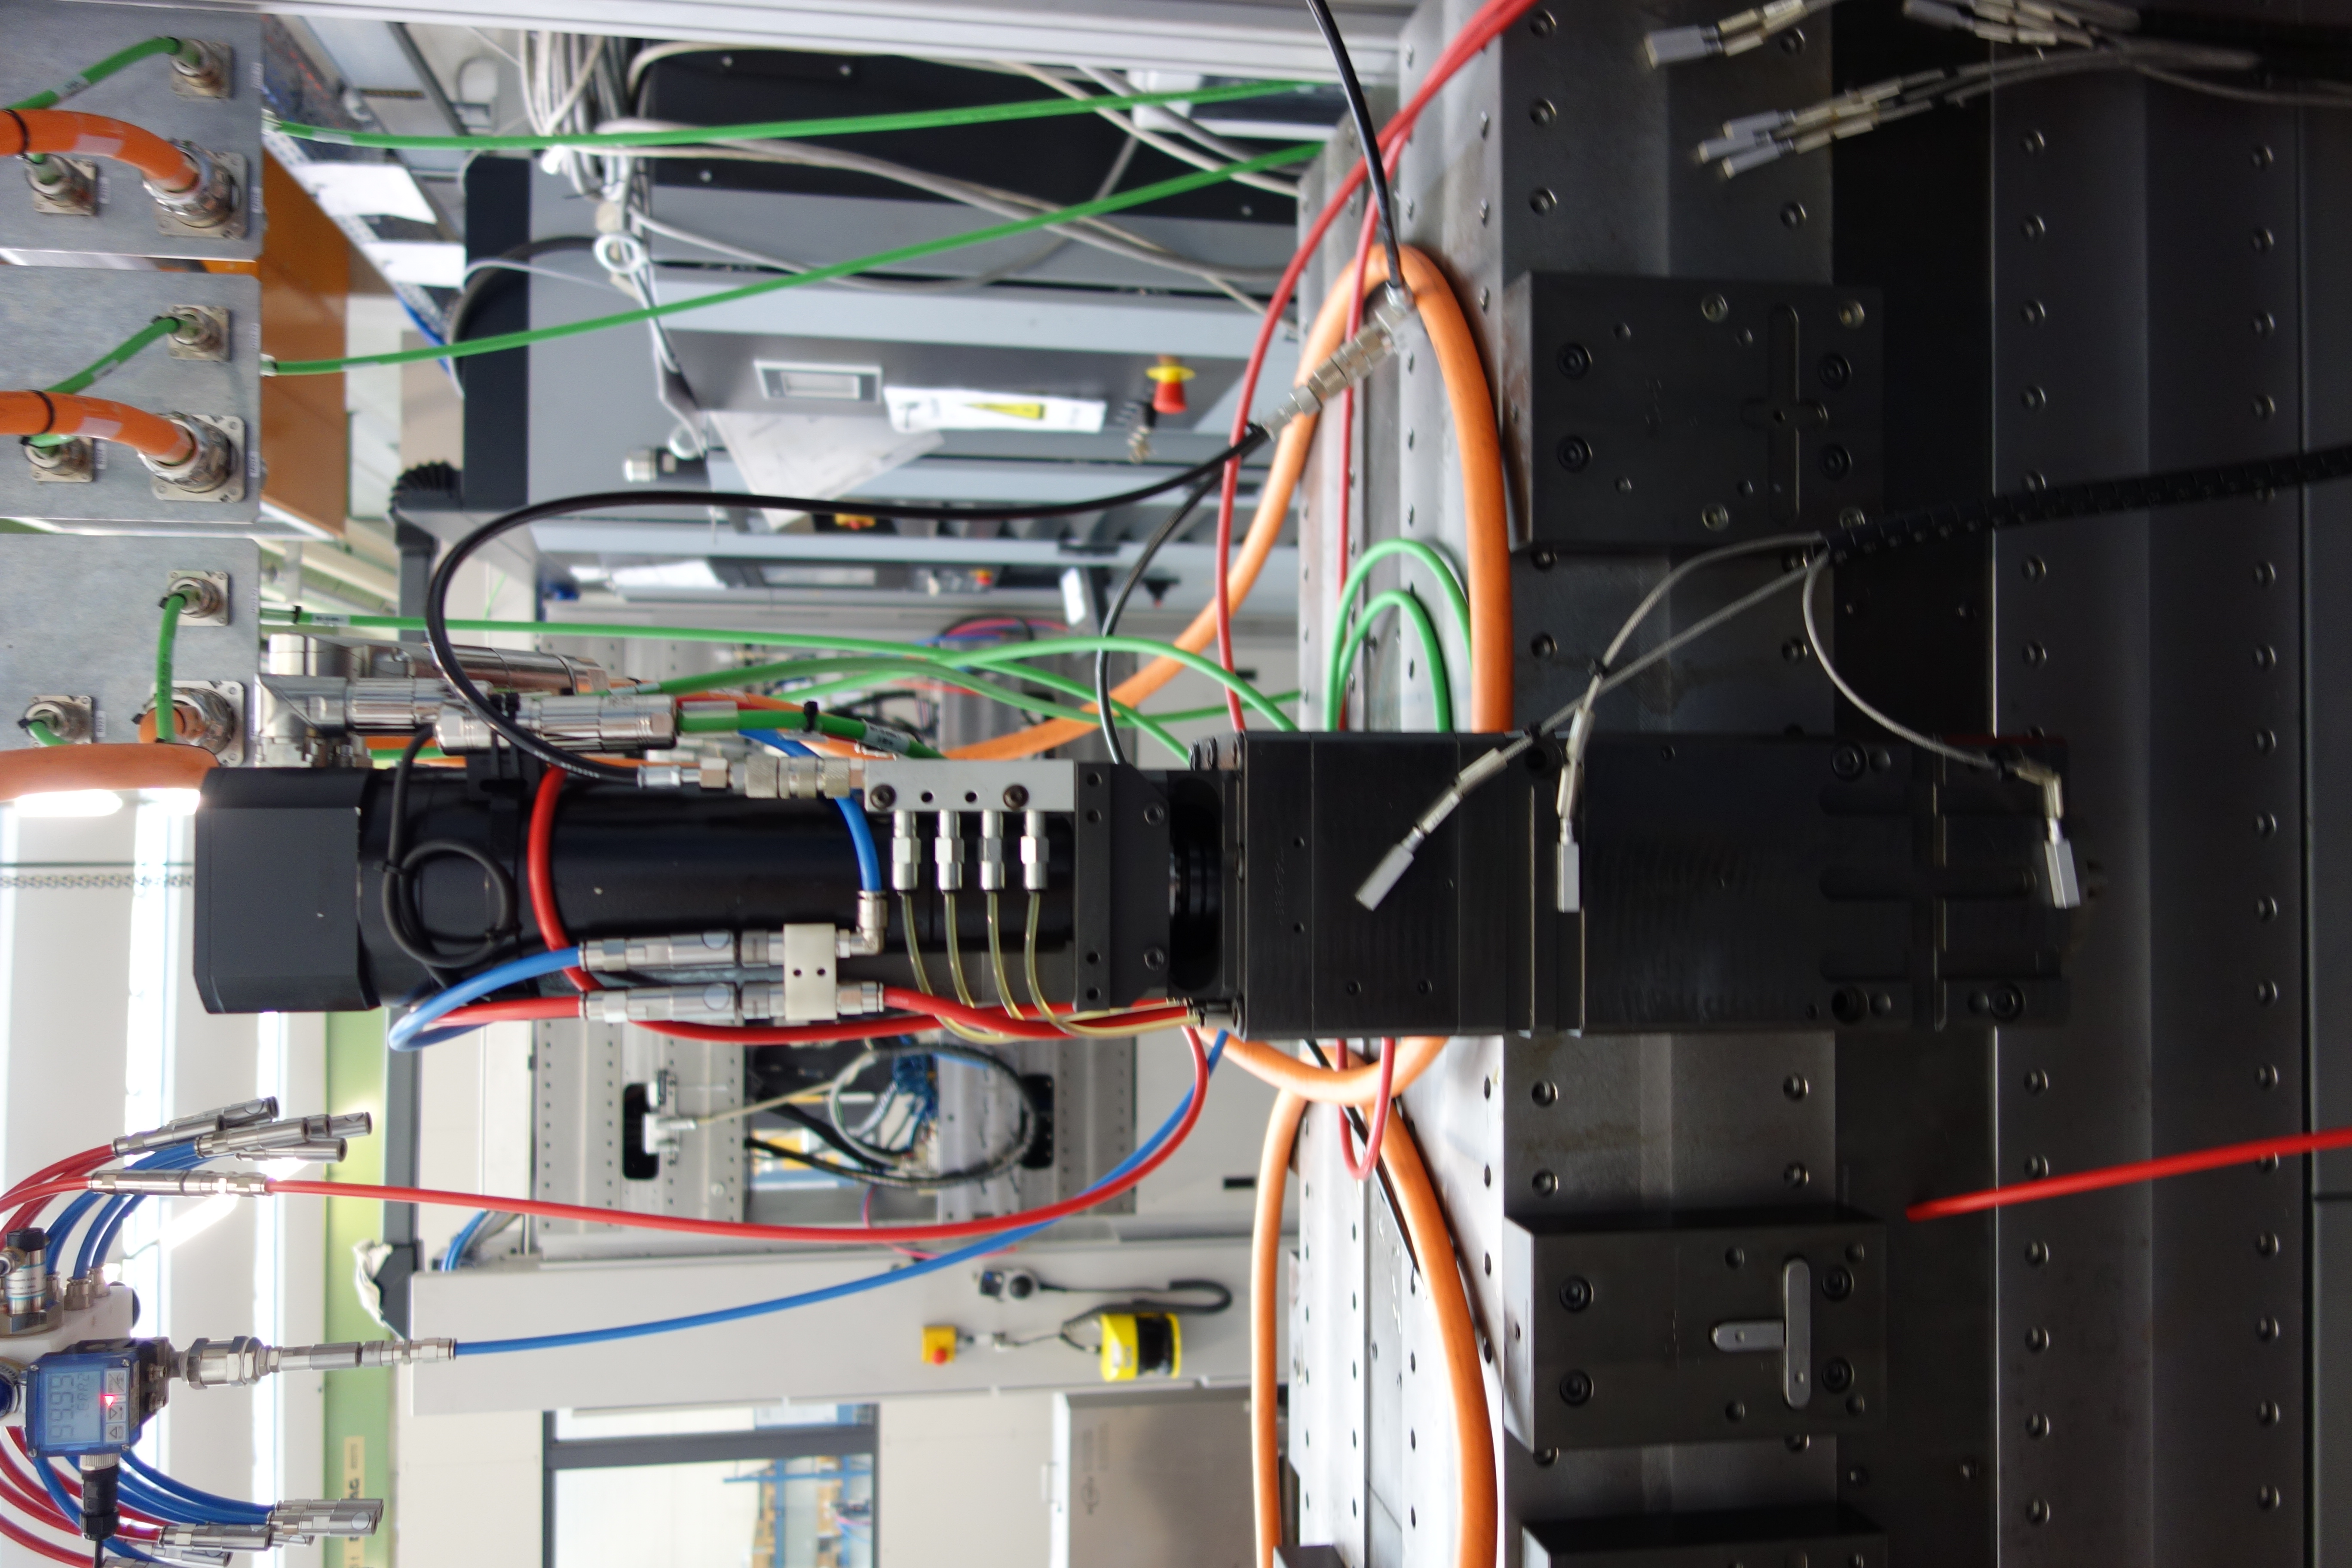
\includegraphics[trim=5cm 5cm 5cm 5cm, clip=true, height=0.3\textwidth, angle=270]{Temperatursensoren_reales_Bild}
%\caption{NCA 5 Bereit zum Testlauf}
%\label{fig:NCA_5_Bereit_zum_Testlauf}
%\end{figure}


\begin{figure}[H]
\centering
\includegraphics[width=0.7\textwidth]{NCA4_Positionen_Temperatursensoren} % Bild der Temperatursensoren
\caption{Position der Temperatursensoren} 
\label{fig:Position_der_Temperatursensoren}
\end{figure}

Der Verlauf der gemessenen Temperatur für das gesamte Testprogramm ist in Abbildung~\ref{fig:Einlauf_Temperaturanzeige} zu sehen.  Durch die Kühlung des Aggregates ist der Temperaturanstieg gering. Die der Abbildung zugrunde liegenden Werte werden im normalen Testlauf zwar in der gleichen Form erfasst wie in der Abbildung dargestellt, aber nicht abgespeichert. Deshalb werden sie im Rahmen dieser Arbeit gesondert aufgezeichnet, um den Temperaturverlauf darstellen zu können. Bei der hier gezeigten Messung wird somit jede Minute ein Messwert mit einer nominalen Auflösung von einem Zehntel Kelvin aufgezeichnet.

\begin{figure}[H]
\begin{tikzpicture}
 \begin{axis}[
 	no markers,
 	% ymin=0,
    xmin=0,
    xmax=96,
 	width=\textwidth,height=0.4\textheight,
  	%title=Einfahrzyklus Drehmomentprofil,
    xlabel={Zeit in min},
    ylabel={Temperatur in $^\circ$C},
    grid=major,
    legend entries={Sensor Lager,Sensor Gehäuse,Sensor Abstreifer},
    legend pos=south east,
    %enlarge x limits=0.01,
]
 	\addplot table[x=Punkte:, y=Temperatursensor1]  {graphen/CSV_Daten/Trendanzeige_Temperatur_Aggregat38207.txt};
 	\addplot table[x=Punkte:, y=Temperatursensor2]  {graphen/CSV_Daten/Trendanzeige_Temperatur_Aggregat38207.txt};
 	\addplot table[x=Punkte:, y=Temperatursensor3]  {graphen/CSV_Daten/Trendanzeige_Temperatur_Aggregat38207.txt};
 \end{axis}
\end{tikzpicture}

% StromLauf1
\caption{Temperaturverlauf an der Außenseite während des Testprogramms bei dem Aggregat mit der Seriennummer 38207}
\label{fig:Einlauf_Temperaturanzeige}
\end{figure}


\subsection{Motortemperatur} \label{cha:Einlaufen_Motortemperatur}

Der Motor besitzt einen eingebauten Temperatursensor. Dieser Wert wird von der Steuerung ausgelesen und kann im Display der Steuerung als Zahlenwert dargestellt werden. Als Messwert wird hierbei der höchste Wert während der letzten Minuten der ersten drei Zyklen aufgezeichnet. 

\section{Auswertung des bisherigen Testablaufs}

Die während der Tests der Aggregate erfassten Daten wurden vom Betrieb bisher nicht ausgewertet. Eine Auswertung wird im Rahmen dieser Arbeit, wie nachfolgend dargestellt, angestrebt. Dabei wird nachfolgend analysiert, ob es sinnvoll ist, diese Messungen durchzuführen und diese Daten zu erfassen, wie aussagekräftig sie sind und welche Rückschlüsse auf die Funktionsfähigkeit der NCAs aus dem derzeitigen Testprogramm gezogen werden können. So werden die Daten für Stromstärke, Motortemperatur und die Temperatur an der Außenseite der NC-Aggregate herangezogen, um das momentane Testverfahren zu analysieren.

Um eine genügend große Anzahl an Messwerten zu erhalten, erfolgt die Auswertung nur aufgrund der Größentypen der NCAs (NCA 2 - 4) und nicht nach dem wesentlich aussagekräftigeren Baustand, der anhand der Artikelnummer ermittelt werden kann. (vergleiche Anhang~\ref{cha_Anhang_4})



\subsection{Stromstärke}

Ein mögliches Auswertungskriterium der bisher erfassten Daten ist die Stromaufnahme des Motors. Diese wird vom Regler erfasst und, wie unter Kapitel~\ref{ch:Ermittelte_Messwerte_Stromstaerke} beschrieben, aufgezeichnet.

Für die Auswertung werden die Messwerte aller seit 2013 getesteten NCAs in Histogrammen dargestellt. Die Klassenbreite beträgt hierbei 0,1 A. Von der üblichen Darstellungsweise in Balkenform wird abgewichen, um die Verschiebung von Zyklus zu Zyklus leichter erkennen zu können.


% Für die Auswertung werden die Messwerte aller seit 2013 getesteten NCAs in Ampere von zwei Stellen nach dem Komma auf eine Stelle nach dem Komma gerundet. Dann wird jeweils die Anzahl der Aggregate ermittelt, die die gleiche Stromaufnahme besitzen. Zur besseren Anschaulichkeit werden die Punkte miteinander verbunden. Von der üblichen Darstellungsweise als Histogramm wird somit abgewichen, um die Verschiebung 

Dies ergibt somit für die NCA2 - NCA5 jeweils 4 Kurven, je eine pro Testzyklus. Diese sind in den Abbildungen ~\ref{fig:Stromaufnahme_NCA_2}, ~\ref{fig:Stromaufnahme_NCA_3}, ~\ref{fig:Stromaufnahme_NCA_4} und ~\ref{fig:Stromaufnahme_NCA_5} zu finden. Wie zu erwarten, steigt die benötigte Stromstärke bei zunehmender Geschwindigkeit. Manche Werte scheinen nicht besonders plausibel (vergleiche NCA 3, Zyklus 3 in Abbildung ~\ref{fig:Stromaufnahme_NCA_3}). Dies könnte zum Beispiel durch eine fehlerhafte Messung verursacht sein.

In allen vier Abbildungen ist der Rückgang der benötigten Stromstärke von Zyklus 1 auf Zyklus 4, der zur Kontrolle dient, zu erkennen. Diese bei gleichen Parametern gemessenen Werte spiegeln den Einlaufvorgang des Rollengewindetriebes wider. Nach dem Einlaufen wird somit für die gleiche Verfahrbewegung weniger Strom und somit weniger Energie benötigt. Dadurch lässt sich zeigen, dass ein erfolgreiches Einlaufen des Rollengewindetriebes stattgefunden hat.

Grundsätzlich ist mit der Messung der Stromstärke somit eine Schwergängigkeit der Aggregate feststellbar. Entsprechend hohe Werte würden dazu Anlass geben, das Aggregat nochmals genauer zu betrachten. Hierzu sind allerdings keine Fälle dokumentiert.

Bei den NCA 4 Aggregaten sind für jeden Zyklus zwei voneinander getrennte Spitzen in den Graphen zu erkennen. (vgl. Abbildung~\ref{fig:Stromaufnahme_NCA_4}) Bei einer genaueren Betrachtung der Daten ist dies auf eine konstruktive Änderung der NCA 4 Achsen zurückzuführen. Zukünftig sollte deshalb eine getrennte Analyse der unterschiedlichen Bautypen erfolgen.


\begin{figure}[H]
\begin{tikzpicture}
 \begin{axis}[
 	ymin=0,
    xmin=0,
 	width=\textwidth,height=0.26\textheight,
  	%title=Stromaufnahme NCA 2,
    xlabel={Stromstärke in A},
    ylabel={Anzahl der Aggregate},
    grid=major,
    legend entries={Zyklus 1,Zyklus 2,Zyklus 3,Zyklus 4},
    enlarge x limits=0.01,
]
 	\addplot+[mark=*] table[x=Ampere, y=Zyklus1]  {graphen/Stromauswertung_Einfahrzyklus_NCA2.csv};
    \addplot+[mark=x] table[x=Ampere, y=Zyklus2] {graphen/Stromauswertung_Einfahrzyklus_NCA2.csv};
    \addplot+[mark=+] table[x=Ampere, y=Zyklus3] {graphen/Stromauswertung_Einfahrzyklus_NCA2.csv};
    \addplot+[mark=asterisk] table[x=Ampere, y=Zyklus4] {graphen/Stromauswertung_Einfahrzyklus_NCA2.csv};
 \end{axis}
\end{tikzpicture}
\caption{Anzahl der NCA 2 mit ihrer jeweiligen maximalen Stromstärke in den 4 Testzyklen}
\label{fig:Stromaufnahme_NCA_2}
\end{figure}



\begin{figure}[H]
\begin{tikzpicture}
 \begin{axis}[
 	ymin=0,
    xmin=0,
 	width=\textwidth,height=0.26\textheight,
  	%title=Stromaufnahme NCA 3,
    xlabel={Stromstärke in A},
    ylabel={Anzahl der Aggregate},
    grid=major,
    legend entries={Zyklus 1,Zyklus 2,Zyklus 3,Zyklus 4},
    enlarge x limits=0.01,
]
 	\addplot+[mark=*] table[x=Ampere, y=Zyklus1]  {graphen/Stromauswertung_Einfahrzyklus_NCA3.csv};
    \addplot+[mark=x] table[x=Ampere, y=Zyklus2] {graphen/Stromauswertung_Einfahrzyklus_NCA3.csv};
    \addplot+[mark=+] table[x=Ampere, y=Zyklus3] {graphen/Stromauswertung_Einfahrzyklus_NCA3.csv};
    \addplot+[mark=asterisk] table[x=Ampere, y=Zyklus4] {graphen/Stromauswertung_Einfahrzyklus_NCA3.csv};
 \end{axis}
\end{tikzpicture}
\caption{Anzahl der NCA 3 mit ihrer jeweiligen maximalen Stromstärke in den 4 Testzyklen}
\label{fig:Stromaufnahme_NCA_3}
\end{figure}



\begin{figure}[H]
\begin{tikzpicture}
 \begin{axis}[
 	ymin=0,
    xmin=0,
 	width=\textwidth,height=0.26\textheight,
  	%title=Stromaufnahme NCA 4,
    xlabel={Stromstärke in A},
    ylabel={Anzahl der Aggregate},
    grid=major,
    legend entries={Zyklus 1,Zyklus 2,Zyklus 3,Zyklus 4},
    enlarge x limits=0.01,
]
 	\addplot+[mark=*] table[x=Ampere, y=Zyklus1]  {graphen/Stromauswertung_Einfahrzyklus_NCA4.csv};
    \addplot+[mark=x] table[x=Ampere, y=Zyklus2] {graphen/Stromauswertung_Einfahrzyklus_NCA4.csv};
    \addplot+[mark=+] table[x=Ampere, y=Zyklus3] {graphen/Stromauswertung_Einfahrzyklus_NCA4.csv};
    \addplot+[mark=asterisk] table[x=Ampere, y=Zyklus4] {graphen/Stromauswertung_Einfahrzyklus_NCA4.csv};
 \end{axis}
\end{tikzpicture}
\caption{Anzahl der NCA 4 mit ihrer jeweiligen maximalen Stromstärke in den 4 Testzyklen}
\label{fig:Stromaufnahme_NCA_4}
\end{figure}



\begin{figure}[H]
\begin{tikzpicture}
 \begin{axis}[
 	ymin=0,
    xmin=0,
 	width=\textwidth,height=0.26\textheight,
  	%title=Stromaufnahme NCA 5,
    xlabel={Stromstärke in A},
    ylabel={Anzahl der Aggregate},
    grid=major,
    legend entries={Zyklus 1,Zyklus 2,Zyklus 3,Zyklus 4},
    enlarge x limits=0.01,
]
 	\addplot+[mark=*] table[x=Ampere, y=Zyklus1]  {graphen/Stromauswertung_Einfahrzyklus_NCA5.csv};
    \addplot+[mark=x] table[x=Ampere, y=Zyklus2] {graphen/Stromauswertung_Einfahrzyklus_NCA5.csv};
    \addplot+[mark=+] table[x=Ampere, y=Zyklus3] {graphen/Stromauswertung_Einfahrzyklus_NCA5.csv};
    \addplot+[mark=asterisk] table[x=Ampere, y=Zyklus4] {graphen/Stromauswertung_Einfahrzyklus_NCA5.csv};
 \end{axis}
\end{tikzpicture}
\caption{Anzahl der NCA 5 mit ihrer jeweiligen maximalen Stromstärke in den 4 Testzyklen}
\label{fig:Stromaufnahme_NCA_5}
\end{figure}




\subsection{Temperatur}



Die Motortemperatur wird durch die Kühlung auf wenige Kelvin konstant gehalten. Somit ist eine aussagekräftige Auswertung dieser Messung nicht möglich.

Auch bei den extern angebrachten Temperatursensoren werden mögliche Unterschiede zwischen den einzelnen Aggregaten durch die Kühlung minimiert. Das Aggregat wird somit auf annähernd konstanter Temperatur gehalten, indem durch einen eventuellen Fehler wesentlich mehr Energie an das Kühlwasser abgegeben werden würde. Außerdem wird die Umgebungstemperatur bei der derzeitigen Datenerfassung nicht berücksichtigt. Dies bedeutet, dass zwei Messungen dieselbe Temperatur anzeigen können, obwohl sich ein Aggregat aufgrund eines Fehlers stärker als ein anderes Aggregat erwärmt hat.



Da die einzelnen aufgezeichneten absoluten Temperaturwerte nicht vergleichbar sind, gibt es keine Möglichkeit, sie aussagefähig auszuwerten.





\section{Analyse des bisherigen Testablaufes} \label{ch:Kritik_Testlauf}






%Verschiedene relevante Faktoren werden durch den momentanen Testablauf erfasst.

Die grundsätzliche Funktionsfähigkeit der NCAs wird dadurch festgestellt, dass im Teststand das erste Mal versucht wird, das Aggregat mithilfe ihrer Steuerung in Gang zu setzen. Dadurch kann man feststellen, ob die Steuerung alle elektrischen Komponenten ansprechen kann, ob sich der Motor wie erwartet ansteuern lässt, das Messlineal verarbeitbare Werte zurückgibt und keines der angeschlossenen Komponenten einen Fehler an die Steuerung meldet. Dabei sind folgende Verbesserungspotentiale denkbar:

\begin{itemize}
    \item Bis jetzt gibt es für alle während der Testphase der NCAs erfassten  Messwerte keine Toleranzen oder Nennwerte. Dies bedeutet, dass zwar die Messwerte bei jedem Aggregat aufgezeichnet werden, es aber aufgrund dieser Werte zu keinen Entscheidungen darüber kommt, ob ein Aggregat voll funktionstüchtig ist oder nicht. 
    \item Aggregate bestehen nur nach subjektiven Kriterien der mit dem Test befassten Mitarbeiter den Testlauf nicht.
    \item Es werden nur sehr grobe Fehler gefunden, z.B. wenn sich das Aggregat nicht über die Steuerung betreiben lässt oder ungewöhnliche Geräusche emittiert. Aus diesem Grund ist mit dem Ende des Testlaufes kein einheitlicher Standard für die Qualität der Achsen sichergestellt. 
    \item Die erkannten Fehler werden nicht durchgängig mitprotokolliert, um daraus eine Fehlerdatenbank aufbauen zu können. Deswegen ist das Wissen über die Fehler sehr stark von den einzelnen Mitarbeitern abhängig und es ist schwierig, bekannte Probleme gezielt abzustellen. 
    \item Außerdem beginnt die Suche nach der Ursache von eigentlich bekannten Problemen immer wieder aufs neue, da unternommene Versuche der Ursachenfindung nicht strukturiert dokumentiert werden.
    \item Da die Aufzeichnung der Messwerte für Motortemperatur, Aggregat-Außenseiten-Tem\-pe\-ra\-tur und Stromstärke per Hand und nicht automatisiert erfolgt, ist die Aufnahme der Messwerte sehr zeitintensiv und aufwendig. Den Mitarbeitern ist schwer zu vermitteln, dass sie die Werte gewissenhaft aufzeichnen, wenn die gemessenen Werte nicht sinnvoll weiter genutzt werden.
    \item Des Weiteren verhindert die Kühlung, dass die Motortemperatur und die Temperatur im Gehäuse des Aggregats stark ansteigt, auch wenn etwas am Motor oder am Gehäuse fehlerhaft ist. Etwaige Fehler können so mithilfe der derzeitigen Temperaturmessungen kaum erkannt werden.
    \item Durch den derzeitigen Testablauf ist nicht sichergestellt, dass die NCAs die spezifizierten Eigenschaften (vgl. \cite{VC_1_Betriebsanleitung2015}) erfüllen. 
    \item Die Aggregate werden nicht bis an ihre Leistungsgrenze belastet. Somit ist nicht sichergestellt, dass alle Komponenten den während des Einsatzes vorkommenden starken Belastungen standhalten.
    \item Auch werden derzeit bekannte Fehler nicht mit dem derzeitigen Testablauf erkannt. So gab es mit den getesteten Aggregaten im Nachhinein Probleme, da axiales Spiel in den Aggregaten nicht erkannt wurde.
\end{itemize}


Zusammenfassend ist durch den derzeitigen Testablauf nicht sichergestellt, dass die NCAs die funktionsrelevanten Eigenschaften aufweisen. Deshalb muss die Teststrategie grundlegend überarbeitet werden.

Eine Einlaufphase des Gewinderollentriebs ist unabdingbar notwendig und sie sollte mit der derzeitigen Aufteilung der Zyklen beibehalten werden. Auch wenn die Einlaufzyklen beibehalten werden, müssen die derzeit damit verbundenen Tests neu gestaltet werden.




% Die bewährte Zyklenaufteilung als Einlaufphase des Gewinderollentriebes sollte auch weiterhin so beibehalten werden. 

%Trotz all der kritischen Punkte kann der derzeitige Testlauf, der praktischer und ökonomischer Weise gleichzeitig als Einlaufphase des Gewinderollentriebes dient, um aussagekräftige Tests erweitert werden. 

%Der Test muss hierfür noch einmal grundlegend überarbeitet werden wobei die bewährte Zyklenaufteilung als Einlauffphase beibehalten werden sollte.

%eine gute Grundlage für weitreichendere Tests. 




\cleardoublepage

\chapter{Grundlagen von Prüfkonzepten für die NC-Aggregate}\label{cha:Grundlagen_von_Pruefkonzepten_fuer_die_NCAs}



In den vorhergehenden Kapiteln werden die NCAs und ihre Eigenschaften, ihre Funktionsstörungen, der bisherige Testablauf und dessen Ergebnisse dargestellt, also der Ist-Zustand dokumentiert. Dabei stellt sich heraus, dass momentan zum Prüfen der NCAs ein Prüfablauf verwendet wird, der nicht ausreicht, um das Ziel der Qualitätssicherung hinlänglich zu gewährleisten. Dies ist in Kapitel~\ref{ch:Kritik_Testlauf} näher dargelegt.



Ein umfassendes Prüfkonzept kann als Grundlage dienen, um die Qualitätssicherung bei einem Prüfobjekt sicherzustellen. Es umfasst dann alle zum Prüfen \cite{DIN1319_1995} notwendigen Schritte. Es sollten deshalb Zeitpunkt der Prüfung, Art der Prüfung, die zu prüfenden Merkmale bzw. Prüfkriterien, die zu prüfende Stichprobe, die Häufigkeit der Prüfung, der damit betraute Personenkreis, die Prüfmittel, das Handling, die Datenerfassung, die Dokumentation, die Datenanalyse, die Bewertung der Analyse und die sich daraus ergebenden notwendigen Konsequenzen in das Konzept einbezogen sein. Ein so weitreichendes Prüfkonzept existiert derzeit für die NCAs nicht.

\section{Grundsätzliche Aspekte von Prüfkonzepten}

Um eine Prüfplanung~\cite{Bernards2005} durchzuführen, d.h. ein umfassendes Prüfkonzept zu erstellen, wie es auch zum Prüfen der NCAs wünschenswert wäre, müssen unterschiedliche Aspekte berücksichtigt werden. So besteht das Prüfen meist aus mehreren einzelnen Tests, bei denen Testaufbau und Testablauf zusammenpassen und aufeinander abgestimmt sind. Um geeignete Prüfverfahren zu finden, sind Messgrößen zu analysieren, Prüfkriterien festzulegen und daraus abgeleitete Tests zu erstellen und zu erproben. Es sollten nicht nur quantitative Tests, bei denen objektiv durch Messen getestet wird, sondern auch qualitative Tests, bei denen subjektiv mit den Sinneswahrnehmungen getestet wird, in die Überlegungen zum Erstellen eines Prüfkonzepts einbezogen werden.

Die mit der Produktion betrauten Mitarbeiter können mit ihren Sinnen wie Sehen, Hören, Riechen oder Tasten Unregelmäßigkeiten im Herstellungsprozess entdecken, was als qualitativer Test in das Prüfkonzept mit eingebunden werden kann. Entsprechende Beobachtungen können erfasst werden, um Fehler zu reduzieren. Dafür muss die Unternehmenskultur so gestaltet sein, dass das Finden und nachhaltige Abstellen von Fehlern Wertschätzung bei den Mitarbeitern bewirkt.


Der Dokumentation sollte innerhalb eines Prüfkonzepts eine wichtige Rolle eingeräumt werden. Sie kann an verschiedenen Stellen ansetzen wie den Prüfgegenständen, dem jeweils betrauten Personal, den Umgebungsbedingungen, den Prüfungen selber, den Messergebnissen und auch der Analyse der Daten. So kann sich die Erstellung einer Fehlerdatenbank, die auch als Fehler-Wissens-Datenbank~\cite{Riebschlaeger2006} bezeichnet werden kann, als hilfreich erweisen. Damit kann erfasst werden, welche Probleme und Fehler wo aufgetreten sind und welche Maßnahmen ergriffen wurden. Damit ist es fundiert möglich, sich mit der Fehlerquelle auseinanderzusetzen. Eine spezielle Software in Form eines CAQ-Systems (Computer Aided Quality Management System) könnte bei der Anlage einer Fehlerdatenbank als probates Hilfsmittel dienen. Eine Dokumentation kann andererseits auch dazu dienen, die Prüfgegenstände qualifizierter einzusetzen. Falls Tests ergeben, dass z.B. ein NC Aggregat höher belastet werden kann, könnte es mit besseren Leistungsdaten an den Kunden weitergegeben werden. 


Wenn die ermittelten und dokumentierten Daten allen relevanten Personenkreisen zur Verfügung stehen, ist eine Verbesserung und Weiterentwicklung des Produkts auf einer fundierten Datenbasis möglich. Dies kann insbesondere helfen, die Arbeit der Konstruktionsabteilung effektiver zu gestalten. Dazu ist es im Bereich der Dokumentation unumgänglich, eine durchgehende eindeutige Kennzeichnung der hergestellten Produkte zu gewährleisten. Wenn dies von der Herstellung über die Tests, die Behebung von Fehlern bis zur Auslieferung an Kunden sichergestellt ist, können die erhobenen, festgehaltenen und ausgewerteten Daten dem Einzelprodukt eindeutig zugeordnet werden. Sollte es z.B. zu Problemen unter den Fertigungsbedingungen beim Kunden kommen, könnte dies der Konstruktionsabteilung wichtige Hinweise zur Verbesserung im Bereich der Konstruktion aber auch der gesamten Herstellung geben, wenn es diese stringente Kennzeichnung innerhalb der Dokumentation gibt.


Damit sichergestellt ist, dass ein Prüfkonzept längerfristig zur Qualitätssicherung beiträgt, sollte es flexibel konzipiert sein, um bei Änderungen im technischen Bereich angepasst zu werden und es sollte eine Evaluierung eingebaut sein, um es regelmäßig zu überprüfen und gegebenenfalls zu überarbeiten. So können sich Tests als nicht aussagekräftig herausstellen oder es werden geeignetere Tests entwickelt, die bisherige Tests ersetzen sollten.


Weiterhin sind bei der Entwicklung von Prüfkonzepten die einschlägigen gesetzlichen Vorgaben und Sicherheitsvorschriften einzuhalten. 

%So kann sich ein auf den ersten Blick geeigneter Prüfablauf als zu aufwendig oder zu kostenintensiv erweisen und kann deswegen nicht umgesetzt werden.

Da jedes Prüfen mit Kosten verbunden ist, ist eine Kalkulation von Kosten und Nutzen wichtig. Das Prüfkonzept insgesamt, aber auch seine Bestandteile sollten so gestaltet sein, dass es ökonomisch sinnvoll ist. Deshalb mag ein günstiger, nicht optimaler Test eher angeraten sein als ein Test, der zwar alle Fehler entdeckt, aber mit immensen Kosten verbunden ist. Jedoch sind rein ökonomische Überlegungen ungeeignet, wenn man mit dem Prüfen einen hohen Qualitätsstandard sichern will.    



Das Entwickeln eines komplexen Prüfkonzepts ist, neben der rein technischen Umsetzung, eine große Herausforderung, denn ein derartiges Konzept muss vom Betrieb finanziert, unterstützt, genehmigt, aufgebaut, durchgesetzt und durchgeführt werden. Diese Implementierung bedarf einer guten Vorbereitung, einer umfassenden Information aller Ebenen des Betriebes und einer möglichst breiten Einbeziehung der Mitarbeiter, wenn sie erfolgreich sein soll. Dies hängt auch davon ab, von wem das Konzept entwickelt wurde, z.B. ob intern oder extern, welche Ebene des Betriebes damit betraut ist und wo eine Notwendigkeit für das Einführen eines derartigen Konzeptes gesehen wird. Zur Implementierung ist eine Dokumentation des Prüfkonzepts in Form eines Prüfplans möglicher Weise hilfreich. Beim  Erstellen und Verarbeiten von Prüfdaten, die man als Grundlage für qualitätslenkende  Maßnahme ansehen kann, sollte man sich laut~\cite{Hering2013} auf das Notwendige beschränken, damit es von den Mitarbeitern akzeptiert wird.



\section{Anforderungen an die Prüfungen}\label{cha:Anforderungen_an_die_Pruefungen}

Der zentrale Bestandteil jedes Prüfkonzepts ist das Testen, das aus einer einzelnen Prüfung oder mehreren gleichen oder unterschiedlichen Prüfungen bestehen kann. So gibt es verschiedenste Tests und Methoden, um herauszufinden, ob die NCAs die notwendigen Eigenschaften (vgl. Kapitel~\ref{Eigenschaften_der_Aggregate}) aufweisen und somit die vorgeschriebenen Anforderungen erfüllen. Bei der Auswahl der Methoden muss darauf geachtet werden, dass man die erwarteten Ziele erreicht. Für die Prüfung in der Serienfertigung ist es besonders wichtig, dass die Methoden sehr effizient und zielgerichtet sind.


Für die Auswahl von Messmethoden in der Serienfertigung sind die in Tabelle~\ref{fig:Randbedingungen_bei_der_Auswahl_von_Messmethoden_in_der_Serienfertigung} aufgeführten Randbedingungen zu beachten. So sollten die Methoden automatisierbar und dokumentierbar sein, keinen großen Personaleinsatz erfordern und nicht zuletzt wirtschaftlich sein. Für die Mitarbeiter sollen die Tests einfach zu bedienen sein und die Mitarbeiter sollen eine klare, einfache Entscheidungsgrundlage haben. Zudem sollten die Messmethoden den Produktionsprozess nicht wesentlich verlängern, so dass eine kurze Durchlaufzeit anzustreben ist. Wie in allen sonstigen Bereichen ist streng darauf zu achten, dass bei allen Messmethoden die gesetzlichen Vorschriften eingehalten werden.











\begin{table}[H]
\center
\fbox{
\begin{minipage}[c]{0.8\textwidth}
\vspace{5pt}
\begin{itemize}
 \item kostengünstig
 \item automatisierbar
 \item gut dokumentierbar
 \item geringer Personaleinsatz
 \item einfache Bedienbarkeit
 \item klare, einfache Entscheidungsgrundlage
 \item kurze Durchlaufzeit
 \item Einhalten gesetzlicher Vorschriften
\end{itemize}

\par\vspace{2pt}
\end{minipage}}
\caption{Randbedingungen bei der Auswahl von Messmethoden in der Serienfertigung}
\label{fig:Randbedingungen_bei_der_Auswahl_von_Messmethoden_in_der_Serienfertigung}
\end{table}















\section{Tests in der Versuchsabteilung}\label{cha_Tests_in_der_Versuchsabteilung}

Wie in Kapitel~\ref{cha:Entdecker_von_Funktionsstoerungen} beschrieben, werden die Prototypen der Aggregate in der Versuchsabteilung während der Konstruktionsphase einem Prototypentest unterzogen. Bei diesem werden verschiedene, von der Konstruktionsabteilung vorgegebene Tests durchgeführt. Ziel dieser Tests ist es, die Tauglichkeit der Konstruktion festzustellen, damit die anschließend in der Serienfertigung in großer Stückzahl gefertigten NCAs keine Funktionsstörungen aufweisen. Es werden einzelne NCAs mit verschiedenen Testaufbauten getestet, was einen hohen Personalaufwand und vermehrte Umbauzeiten bedeutet. Deswegen sind die Tests aufwändig und zeitintensiv und nicht direkt auf die Serienfertigung anwendbar. Trotzdem können sie wichtige Hinweise geben, was alles getestet werden kann, wie es getestet werden kann und welche Tests über die Jahre entwickelt wurden, um daraus Ansätze für Tests der NCAs in der Serienfertigung abzuleiten.

In Tabelle~\ref{fig:Erfasste Parameter der NCAs in der Versuchsabteilung} sind die Parameter für die Funktionsfähigkeit der NC-Aggregate dargestellt, die die Versuchsabteilung erfasst hat. Diese Parameter werden außer 'Inbetriebnahme möglich' im derzeitigen Testverfahren nicht erfasst.



\begin{table}[h]
\center
\fbox{
\begin{minipage}[c]{0.8\textwidth}
\vspace{5pt}
\begin{itemize}
\item Inbetriebnahme möglich
\item kurzfristige und dauerhafte Spitzenkräfte
\item Leistungsdaten im Leerlauf 
\item Leistungsdaten mit Belastung
\item Bremshaltekraft 
\item Positionier- und Wiederholgenauigkeit
\item axiales und radiales Spiel der Pinole
\item Verhalten bei Dauerbelastung
\end{itemize}
\par\vspace{2pt}
\end{minipage}}
\caption{Erfasste Parameter der NCAs in der Versuchsabteilung}
\label{fig:Erfasste Parameter der NCAs in der Versuchsabteilung}
\end{table}




Tabelle~\ref{fig:Messmethoden_in_der_Versuchsabteilung} zeigt die Messmethoden auf, mit denen die in Tabelle~\ref{fig:Erfasste Parameter der NCAs in der Versuchsabteilung} dargestellten Parameter in der Versuchsabteilung erfasst werden. Dabei kann man z.T. mit einer Messmethode mehrere Parameter erfassen. 




\begin{table}[h]
\center
\fbox{
\begin{minipage}[c]{0.8\textwidth}
\vspace{5pt}
\begin{itemize}
\item Anschließen der Achse an die Steuerung
\item Steuerbarkeit der Achse ohne Fehler
\item Fahren auf Block mit unterschiedlichen Haltezeiten
\item Abfahren des Bewegungsprofils mit Gasdruckfeder als Belastung
\item Abfahren des Bewegungsprofils im Leerlauf 
\item Aufbringen von Kräften, bis die Haltebremse die aufgebrachte Kraft nicht mehr halten kann
\item Messung der Position der Pinole mit Wirbelstromsensoren mit und ohne Belastung
\item Messen des radialen und axialen Spiels durch Aufbringen von Kräften
\end{itemize}
\par\vspace{2pt}
\end{minipage}}
\caption{Messmethoden in der Versuchsabteilung}
\label{fig:Messmethoden_in_der_Versuchsabteilung}
\end{table}


%Kurze Analyse der Messmethoden aus Tabelle~\ref{fig:Messmethoden_in_der_Versuchsabteilung}. Genauere Darstellung in Kapitel~\ref{cha:Pruefkonzepte} falls Messmethode interressant Aussuchen welche Tests für die Serienprüfung interessant sind


Mit der Methode des 'Anschließens der Achse an die Steuerung' wird der Parameter 'Inbetriebnahme möglich' getestet. Es handelt sich bei diesem Test wie in Kapitel~\ref{ch:Kritik_Testlauf} erläutert, um die Grundvoraussetzung zum Betreiben der NCAs. Man kann feststellen, ob die Achse ohne Fehler betrieben werden kann. Dieser grundlegende Test ist somit nicht nur in der Ver\-suchs\-pha\-se enthalten, sondern auch im bisherigen Prüfverfahren, und ist aus keinem Prüfkonzept wegzudenken.



%wird derzeit im Serientest nicht gemacht. interessante Methode um Belastungen zu testen, Spitzenlasten und Dauertest, Leistungsdaten mit Belastung. näheres in Kapitel~\ref{cha:Fahren auf eine Feder oder auf Block}


Mit den beiden Messmethoden 'Fahren auf Block mit unterschiedlichen Haltezeiten' und dem 'Abfahren eines Bewegungsprofils mit Gasdruckfeder' handelt es sich um Belastungstests, also um Tests, bei denen die Pinole höheren Kräften ausgesetzt ist. Man kann damit sowohl die in Tabelle~\ref{fig:Erfasste Parameter der NCAs in der Versuchsabteilung} aufgeführten Parameter der 'kurzfristigen und dauerhaften Spitzenkräfte' testen genauso wie den Parameter 'Leistungsdaten mit Belastung' als auch den Parameter 'Verhalten bei Dauerbelastung'. Es ist eine interessante Messmethode, um Leistungsdaten mit Belastung zu testen. Deshalb wird sie im Kapitel~\ref{cha:Fahren auf eine Feder oder auf Block} als mögliche Testmethode aufgeführt.

%Spitzenlasten und Dauertest, Leistungsdaten mit Belastung

Die Messmethode 'Abfahren von Bewegungsprofilen im Leerlauf' wird nicht nur im Versuchsbereich eingesetzt, sondern auch in den derzeit benutzten Prüfungen gefahren, um die 'Leistungsdaten im Leerlauf' zu messen. Da sich die Messung mit geringem Aufwand durchführen lässt und hilfreiche Leistungsdaten liefert, ist zu erwägen, ob sie in einem neuen Prüfkonzept für die NCAs enthalten sein sollte (Vergleiche Kapitel~\ref{cha:Abfahren eines Profils im Leerlauf}). Darüber hinaus ist erwägenswert, ob mit dieser Messmethode durch weitere Messungen oder durch Änderungen am Fahrprofil weitreichendere Informationen zur Funktionsfähigkeit der NCAs zu gewinnen wären.





%Abfahren von Bewegungsprofilen im Leerlauf. wird derzeit schon gemacht. ist auch weiter interessant, geringer Aufwand. Vergleiche Kapitel~\ref{cha:Abfahren eines Profils im Leerlauf}, Leistungsdaten



Während der Entwicklungsphase der NCAs ist das Testen der Haltebremse und deren Bremshaltekraft wichtig. Getestet wird, indem man so starke Kräfte aufbringt, bis die Haltebremse die aufgebrachte Kraft nicht mehr halten kann. Es handelt sich um einen sehr aufwendigen Test wie in Kapitel~\ref{cha_Messung_der_Bremshaltekraft} ausgeführt.

%Da derzeit keine Probleme mit der Haltebremse bekannt sind, besteht keine Notwendigkeit, diesen aufwendigen Test für das Prüfkonzept in der Serienfertigung vorzuschlagen.


%Messung der Haltebremse, Bremshaltekraft, Aufbringen von Kräften bis die Haltebremse die aufgebrachte Kraft nicht mehr halten kann, Derzeit keine Probleme mit der Haltebremse, deswegen derzeit nicht in der Serienfertigung nötig.






In Tabelle~\ref{fig:Messmethoden_in_der_Versuchsabteilung} ist die 'Messung der Position der Pinole mit Wirbelstromsensoren mit und ohne Belastung' als Messmethode während der Entwicklungsphase der NCAs zu finden, um den Parameter 'Positionier- und Wiederholgenauigkeit' (siehe Tabelle~\ref{fig:Erfasste Parameter der NCAs in der Versuchsabteilung}) zu testen. Dabei wird das wiederholte Anfahren derselben Position mithilfe von Wirbelstromsensoren gemessen. Es handelt sich um eine aufwendige externe Messung, deren Ergebnisse mehr von den Einstellungen des Motorreglers abhängen als vom Aggregat selber. Darüber hinaus können beim Zweigebersystem Unregelmäßigkeiten direkt erkannt werden. Deshalb kommt diese Messung nicht in die engere Wahl für einen Test in der Serienprüfung.




%an Motorgeber Einstellungen abhängig als vom Aggregat selber. Aufwendige externe Messun Erfahrungsgemäß mehr von den Motorgeber Einstellungen abhängig als vom Aggregat selber. Aufwendige externe Messung. Durch zweigeber System kann auch so unregelmäßigkeiten festgestellt werden.






Mit dem 'Messen des radialen und axialen Spiels' durch Aufbringen von Kräften soll der Parameter 'axiales und radiales Spiel der Pinole' gemessen werden. Zu diesem Verfahren wurden Untersuchungen im Betrieb gemacht und ein fertiges Konzept entwickelt. Jedoch kommt das Verfahren beim derzeitigen Testen nicht zum Einsatz. Es ist sehr zeit-, personal- und kostenaufwendig und bringt keinen diesem Aufwand adäquaten Informationsgewinn. Deshalb erfüllt es die Kriterien zur Auswahl von Messmethoden in der Serienfertigung (Tabelle~\ref{fig:Randbedingungen_bei_der_Auswahl_von_Messmethoden_in_der_Serienfertigung}) nicht.




\section{Erweiterung der Messgrößen}\label{cha_Moegliche_Messgroeen}

Außer den in der Versuchsabteilung während der Konstruktionsphase der NCAs erfassten Messgrößen (vgl. Tabelle~\ref{fig:Erfasste Parameter der NCAs in der Versuchsabteilung}) und den in Kapitel~\ref{cha:Ermittelte_Messwerte} beschriebenen, derzeit im Testablauf erfassten Größen, Temperatur mit außen auf den Achsen aufgesetzten Temperatursensoren, Motortemperatur und maximale Stromstärke bei konstanter Geschwindigkeit, gibt es weitere eventuell neu zu entwickelnde Testverfahren, Messmethoden und Messgrößen, bei denen abzuwägen ist, ob sie als Bestandteil eines Prüfkonzeptes sinnvoll sind. Denn aus Kapitel~\ref{ch:Kritik_Testlauf} ist ersichtlich, dass das zur Zeit angewandte Testverfahren einer Umgestaltung bedarf.

Als Grundlagen für diese Umgestaltung sind Recherchen durchzuführen, die über das Analysieren der in der Versuchsabteilung gefahrenen Tests hinausgehen. Aus ihnen ergibt sich, dass Messgrößen aus unterschiedlichen Bereichen einbezogen werden müssen.

% Als Grundlagen für diese Umgestaltung zu schaffen, ist es notwendig, Recherchen über das Analysieren der in der Versuchsabteilung gefahrenen Tests hinaus durchzuführen. Aus ihnen ergibt sich, dass Messgrößen aus unterschiedlichen Bereichen einbezogen werden müssen.

\begin{itemize}
 \item  Insbesondere kämen als mögliche Messung Schwingungsfrequenzanalysen in Frage, denn mit Schwingungsmessungen können im Maschinenbau Rückschlüsse auf Eigenschaften bzw. Unstimmigkeiten gezogen werden.
 
 \item Ähnlich verhält es sich mit Akustikmessungen, die generell bei der Abnahme von Maschinen verwendet werden. 
 
 \item Temperaturmessungen sind eine weitere bewährte Prüfmethode, denn sie liefern Daten zum thermischen Verhalten und zum Energieumsatz, wobei eine erweiterte Termperaturmessung einen Fehler aufzeigen könnte. 
 
 % \item Als mögliche Messgröße kämen Schwingungsfrequenzen in Frage, da man im Maschinenbau allgemein damit Rückschlüsse auf Eigenschaften bzw. Unstimmigkeiten zieht. Ähnlich verhält es sich mit Schallmessungen, die generell bei der Abnahme von Maschinen verwendet werden. Temperaturmessungen sind eine weitere bewährte Prüfmethode und sie würden Daten zum thermischen Verhalten und zum Energieumsatz liefern, wobei eine Temperaturerhöhung auf einen Fehler hindeuten könnte. 
 
 \item Mit Durchflussmessungen könnte man die Funktionsfähigkeit von Kühlung und Schmierung überprüfen. Auch das Überprüfen der Dichtigkeit der Schmierung wäre ein Ansatzpunkt für einen Test, der optimaler Weise über einen längeren Zeitraum wiederholt durchgeführt werden sollte.
 
 \item Tests in Bezug auf mechanisches Spiel würden Aussagen zur mechanischen Präzision liefern. Tests zur Wiederhol- und Positioniergenauigkeit wären wichtig für Aussagen über die Prozesssicherheit des Aggregats, da sie Aufschluss über die Steifigkeit und Genauigkeit des Antriebs geben könnten.


 \item Die Dokumentation der von der VC 1 Steuerung während des Betriebes der NCAs erfassten Messgrößen wie Motorstrom und Motortemperatur könnte eine Datengrundlage für die Funktionstüchtigkeit der NCAs liefern.
\end{itemize}


















\begin{comment}

\colorbox{orange}{TEXT in Kap 6}
Von der VC 1 Steuerung werden verschiedene Werte während des Betriebes der NCAs zwar erfasst jedoch nicht angezeigt und dokumentiert wie in Kapitel~\ref{} erklärt. Sie dienen dem präzisen Betreiben der NCAs. Es handelt sich dabei um den Motorstrom, die Motortemperatur, die Fequenz des Erregerfeldes, den Positionswert des Motorgebers und falls vorhanden den Positionswert des Linearmesssystem.

So sind aus dem Motorstrom, wie in Kapitel~\ref{ch:Ermittelte_Messwerte_Stromstaerke} erklärt, indirekt Drehmoment und Kraft bei konstanter Spannung näherungsweise berechenbar. Die Motortemperatur gibt Hinweise auf die thermische Auslastung. Die Frequenz des Erregerfeldes beim Synchronmotor lässt auf die Motordrehzahl und die Winkelposition schließen. Aus dem Positionswert des Motorgebers lässt sich die rotatorische Position des Motors und die Drehzahl berechnen. Und über die Steigung ist die lineare Position der Pinole berechenbar. Mit dem Linearmesssystem beim 2-Gebersystem (vgl. Kapitel~\ref{cha:Unterschiede der NC-Aggregate}) wird die lineare Position der Pinole bestimmt.

Wenn man durch eine erweiterte Dokumentation dieser von der VC 1 erfassten Werte die so geschaffene Datengrundlage während des möglichen Prüfprozesses auswerten könnte, ließen sich daraus wichtige Kennwerte der NCAs ableiten. Diese ständen als Testwerte für Aussagen über die Funktionsfähigkeit der NCAs zur Verfügung ohne dass externe Messeinrichtungen nötig wären.


\colorbox{orange}{für Kap 6 text}

iNBETRIEBNAHME



\section{}


Aus den Vorüberlegungen zu möglichen Tests für die NCAs, ergeben sich Prüfungen, die an NCAs auf dem derzeitigen Prüfstand im Rahmen dieser Arbeit versuchsweise durchgeführt werden.
Dabei handelt es sich um:






Abfahren eines Profils unter Belastung
Fahren auf eine Feder oder auf Block
Anhängen eines Gewichtes oder einer Last
Abfahren eines Profils im Leerlauf
Langsames Abfahren im Trapezprofil
Abfahren im Stufenprofil
Abfahren im Maximalprofil Polynom 5 Ordnung
Schwingungsmessung
Temperaturmessung
Messung der Motortemperatur
Messung der Temperatur mit externen Sensoren
Volumenstrommessung
Volumenstrommessung des Kühlwassers    
Volumenstrommessung des Schmieröls
Messung der Bremshaltekraft

\end{comment}

\cleardoublepage

%\end{comment}
%\chapter{Prüfansätze}\label{cha:Pruefkonzepte}





Das nachfolgende Kapitel enthält Versuche und Überlegungen zu möglichen Messungen, um die im Kapitel~\ref{Eigenschaften_der_Aggregate} dargestellten Eigenschaften der Aggregate messtechnisch zu erfassen. Aus den Vorüberlegungen zu möglichen Tests für die NCAs (vgl. Kapitel~\ref{cha:Grundlagen_von_Pruefkonzepten_fuer_die_NCAs}) ergeben sich konkrete Prüfungen, die an NCAs auf dem derzeitigen Prüfstand im Rahmen dieser Arbeit versuchsweise durchgeführt werden. Denn wie in Kapitel~\ref{ch:Kritik_Testlauf} geäußert, reicht der derzeitige Testlauf nicht aus, um die verschiedenen Fehler beim Produktionsprozess der NCAs aufzudecken.



\section{Abfahren eines Profils unter Belastung}

Um die Belastungen der NCAs in der Produktion zu simulieren, können sie für die Testläufe extern belastet werden. Entweder kann die Achse auf Federn oder auf einen Block ausfahren oder es wird zur Belastung ein zusätzliches Gewicht an der Achse angebracht.



\subsection{Fahren auf eine Feder oder auf Block}\label{cha:Fahren auf eine Feder oder auf Block}


 
Eine Möglichkeit, viele Funktionen der NCAs auf einmal zu messen, ist, mit der Pinole der Achse auf eine Last zu fahren. Diese Art der Prüfung wird bereits bei der Erstmusterprüfung im Versuch praktiziert. Es kann entweder gegen Gasdruckfedern (vgl. Abbildung~\ref{fig:Fahren_auf_Feder}) oder auf Block (vgl. Abbildung~\ref{fig:Fahren_auf_Block}), d.h. gegen einen festen Widerstand (Metallklotz) gefahren werden. Mit dieser Messmethode kann sehr einfach überprüft werden, ob ein NCA die geforderten Kräfte aushalten kann.


%\colorbox{orange}{Bild einfügen}

\begin{figure}[H]
\centering
\begin{minipage}[b]{0.47\textwidth}
\centering
\includegraphics[width=\linewidth]{Fahren_auf_Block} 
\caption{Konzept: auf Block fahren} 
\label{fig:Fahren_auf_Block}
\end{minipage}
\begin{minipage}[b]{0.47\textwidth}
\centering
\includegraphics[width=\linewidth]{Fahren_auf_Feder} 
\caption{Konzept: Fahren auf eine Feder} 
\label{fig:Fahren_auf_Feder}
\end{minipage}

%\caption{Konzept Fahren auf Block und Feder}
%\label{fig:Fahren_auf_Block_und_Feder}
\end{figure}



Hierbei sind folgende Kriterien, die für oder gegen diese Messmethode im Serieneinsatz sprechen, abzuwägen:

Pro:
\begin{itemize}
 \item Statische Haltekräfte können nur auf diese Weise überprüft werden
 \item Entspricht einem realen Belastungsfall
 \item Absolute Positioniergenauigkeit und Wiederholgenauigkeit kann unter Belastung erfasst werden
\end{itemize}


Contra:
\begin{itemize}
 \item Hoher Aufwand
 \item Messung kann nicht ohne großen mechanischen Aufwand an anderen Maschinen als den Testmaschinen durchgeführt werden
  \item Arbeitssicherheit ist beim Testen schwer zu gewährleisten
  \item Belastungen können auch durch dynamische Kräfte abgebildet werden. Zur maximalen Auslastung des Aggregates ist das Fahren auf eine Last nicht erforderlich. (vgl.~\ref{cha:Polynom_5_Ordnung}) 
  \item Durch Schleppfehler kann das Spiel der Aggregate, auch ohne auf Belastung zu fahren, gemessen werden.
  \item Die absolute Positionierung des Aggregates (Positioniergenauigkeit) ist wesentlich stärker davon abhängig, ob auf Last gefahren wird, als die Wiederholgenauigkeit. Für den Einsatz ist die Wiederholgenauigkeit sehr viel wichtiger als die absolute Positioniergenauigkeit. 
  \item Es ist eine aufwendige Mechanik nötig, um verschiedene Hublängen messen zu können.
\end{itemize}

Als Fazit ergibt sich, dass man durch das Fahren auf Last nur wenige Erkenntnisse gewinnt, die man nicht auch auf andere Weise erlangen kann. Diese wenigen Erkenntnisse erfordern einen hohen Aufwand. Deshalb wird dieser Ansatz für die Umsetzung im Teststand für die Serienprüfung nicht weiter verfolgt.


% Der zusätzliche Gewinn an Erkenntnissen durch das Fahren auf Last wird durch die Gegenargumenten nicht gerechtfertigt.

\subsection{Anhängen eines Gewichtes oder einer Last}

Neben der Möglichkeit, mit der Achse auf eine Last zu fahren, kann auch durch das Anhängen einer Prüfmasse das Fahrverhalten verändert werden. Durch das veränderte Verhalten der Achse ist es möglich, neue Erkenntnisse zu gewinnen. Mit einem entsprechend hohen Gewicht kann man die Achse bis an ihre Grenzen belasten (siehe Abbildung~\ref{fig:NCA_mit_Zusatzgewicht}).

\begin{figure}[h]
\centering
\includegraphics[width=0.4\textwidth]{NCA_mit_Zusatzgewicht} 
\caption{Konzept: Anhängen eines Zusatzgewichtes} 
\label{fig:NCA_mit_Zusatzgewicht}
\end{figure}



Wie aus Tabelle~\ref{tab:Traegheitsmoment_durch_Zusatzlast} ersichtlich, ändert diese Methode nur bei den kleinen NCAs wie den NCA 2 das Betriebsverhalten signifikant.

%Das Massenträgheitsmoment der Aggregate ohne Zusatzmasse ist der Übersichtstabelle der Aggregate von Riedle \cite{Riedle2015} zu entnehmen. Diese findet sich im Anhang~\ref{cha_Anhang_4}. Mit der bekannten Spindelsteigung $p$ und einem verwendeten zusätzlichen maximalen Gewicht von $m_{zus} = \SI{20}{\kilogram}$ ergeben sich die in der Tabelle~\ref{tab:Traegheitsmoment_durch_Zusatzlast} ersichtlichen Werte. Die \SI{20}{\kilogram} wurden nach dem Lastenhandhabungsgesetz abgeschätzt. Vergleiche Anhang~\ref{cha_Anhang_5}. Auch wirkt sich nach Formel~\ref{eq:Zusatzlast} die Zusatzmasse $m_{zus}$ bei großen Spindelsteigungen $p$ stärker aus als bei kleinen Gewindesteigungen.

Das Massenträgheitsmoment der Aggregate ohne Zusatzmasse ist der Übersichtstabelle der Aggregate von Riedle \cite{Riedle2015} zu entnehmen. Diese findet sich im Anhang~\ref{cha_Anhang_4}. Mit der bekannten Spindelsteigung $p$ und einem verwendeten zusätzlichen maximalen Gewicht von $m_{zus} = \SI{20}{\kilogram}$ laut Lastenhandhabungsgesetz (vgl. Anhang~\ref{cha_Anhang_5}) ergeben sich die aus der Tabelle~\ref{tab:Traegheitsmoment_durch_Zusatzlast} ersichtlichen Werte. So wirkt sich nach Formel~\ref{eq:Zusatzlast} die Zusatzmasse $m_{zus}$ bei großen Spindelsteigungen $p$ stärker aus als bei kleinen Gewindesteigungen.

%Die \SI{20}{\kilogram} wurden nach dem Lastenhandhabungsgesetz abgeschätzt. Vergleiche Anhang~\ref{cha_Anhang_5}.



\begin{equation}\label{eq:Zusatzlast}
J_{zus} = m_{zus} \cdot \left(\frac{p}{2 \cdot \pi}\right)^2
\end{equation}


\begin{table}[h]
\centering





\begin{tabular}{cccccc}\toprule
Aggregat Sach-Nr. & Aggregat & $p$ & $J_{NCA} $ & $J_{Zus.}$ & Unterschied \\
 &  & \si{\milli\meter} & \SI{e-6}{\kilogram\meter\squared} & \SI{e-6}{\kilogram\meter\squared} & \% \\
 \midrule
100-54-0590.0 & NCA 2 & 16 & 51 & 130 & 254 \\
100-54-0580.0 & NCA 2 & 5 & 42 & 13 & 30 \\
100-54-0592.0 & NCA 2 & 16 & 59 & 130 & 221 \\
100-54-0585.0 & NCA 2 & 16 & 46 & 130 & 283 \\
100-54-0575.0 & NCA 2 & 5 & 39 & 13 & 33 \\
100-54-0720.0 & NCA 3 & 10 & 352 & 51 & 14 \\
100-54-0730.0 & NCA 3 & 25 & 448 & 317 & 71 \\
100-54-0632.0 & NCA 4 & 16 & 1144 & 130 & 11 \\
100-54-0700.0 & NCA 4 & 10 & 1123 & 51 & 5 \\
100-54-0635.0 & NCA 5 & 15 & 4268 & 114 & 3 \\
100-54-0637.0 & NCA 5 & 10 & 4226 & 51 & 1 \\
\bottomrule
\end{tabular}
\caption{Trägheitsmoment durch eine Zusatzlast  $m_{zus}$ von \SI{20}{\kilogram}}
\label{tab:Traegheitsmoment_durch_Zusatzlast}
\end{table}





\section{Abfahren eines Profils im Leerlauf}\label{cha:Abfahren eines Profils im Leerlauf}



Neben der Möglichkeit auf Widerstände zu fahren oder die Achse mit einem Gewicht zu belasten, gibt es auch die Möglichkeit, die Achse im ``Leerlauf'' zu betreiben und so über den Zustand des NCAs Erkenntnisse zu gewinnen. Dabei versteht man unter Leerlauf laut Duden \textquote{das Laufen einer Maschine ohne Belastung} \cite{Duden_Leerlauf}, was in diesem Fall heißt, dass kein Werkzeug angebaut ist, das Arbeit verrichten könnte.

Um die Achsen mit der Steuerung betreiben zu können, müssen viele Daten generiert und verarbeitet werden, die zu einer Auswertung herangezogen werden können. Allerdings sind die meisten dieser Daten nur auf dem Regler vorhanden und können nicht in die VC 1 Steuerung übertragen werden. Mit dem Automation Studio, ein Softwaretools des Herstellers B\&R des Reglers, kann direkt auf dessen Daten zugegriffen werden. 

Dieser Zugriff ist allerdings aufwendig und kompliziert, da hierzu auf die Maschine über einen Fernwartungszugang zugegriffen werden muss. Außerdem ist dies risikoreich, weil mit dem Fernwartungszugang eine komplette Fernsteuerung der Maschine ermöglicht wird. Darüber hinaus können diese Testdaten während des derzeitigen Testablaufs nicht automatisiert erfasst werden. So bietet der direkte Zugriff auf die Daten des Reglers zwar eine Möglichkeit, auf diesem Weg gezielt viele, detaillierte Informationen zu gewinnen, wie es z.B. für die hier vorgestellten Untersuchungen nötig war. Aber man kann über den derzeit sehr aufwändigen und risikobehafteten Zugriff auf den Regler keine Standardmethode für die Erfassung der Daten der Testabläufe in der Serienproduktion entwickeln. Beispiele relevanter Messgrößen, die aus dem Regler ausgelesen werden können zeigt Tabelle~\ref{fig_Beispiele_relevanter_Daten_die_aus_dem_Regler_ausgelesen_werden_koennen}.


\begin{table}[H]
\center
\fbox{
\begin{minipage}[c]{0.6\textwidth}
\vspace{5pt}
\begin{itemize}
\item Positionen von Messlineal und Drehgeber
\item Stromstärke 
\item Drehmoment
\item Errechnete Reglerwerte wie z.B.
\begin{itemize}
\item Soll-Position
\item Sollgeschwindigkeit
\end{itemize}
\item Motortemperatur
\end{itemize}
\par\vspace{2pt}
\end{minipage}}
\caption{Aus dem Regler auslesbare Messgrößen}
\label{fig_Beispiele_relevanter_Daten_die_aus_dem_Regler_ausgelesen_werden_koennen}
\end{table}



Mit dem Automation Studio von B\&R können von den aus dem Regler ausgelesenen Daten sogenannte Traces aufgenommen werden. Dabei werden die ausgewählten Informationen mit einem eingestellten Zeitabstand über einen definierten Zeitbereich ausgelesen. Diese Informationen lassen sich abspeichern und auswerten. Manche dieser Werte (z.B. Stromstärke) werden zwar derzeit an die VC 1 Steuerung übergeben, können aber von dort aus dann nicht abgespeichert werden. 



%Deswegen weisen diese Aggregate ein anderes Fahrverhalten auf.

Neben dem Auslesen der Messgrößen aus dem Regler gibt es darüber hinaus  die Möglichkeit, weitere Messungen an den Aggregaten vorzunehmen, wie es bei den Tests in der Versuchsabteilung gemacht wird. Dafür werden u.a. beim Abfahren eines Profils im Leerlauf weitere Messungen wie z.B. Entfernungsmessungen mit Wirbelstromsensoren vorgenommen.

% Durch das Auslesen der Daten am Regler kann man viele Informationen über die NCAs gewinnen. Jedoch gibt es darüber hinaus die Möglichkeit, weitere Messungen an den Aggregaten vorzunehmen, wie es bei den Tests in der Versuchsabteilung gemacht wird. Dafür werden u.a. beim Abfahren eines Profils im Leerlauf weitere Messungen wie z.B. Entfernungsmessungen mit Wirbelstromsensoren vorgenommen.

Da eine der wichtigsten Funktionen der NCAs das positionsgenaue Abfahren einer Strecke ist, sind Messungen, die mit dem Fahrweg zusammenhängen, erwägenswert. Jedoch sind zusätzliche Wegmessung nur bei Aggregaten mit Ein-Geber-Regelung (vgl. Kapitel~\ref{cha_Steuerung_Aufbau_NCA}) sinnvoll. Bei der Zwei-Geber-Regelung (vgl. Kapitel~\ref{cha_Steuerung_Aufbau_NCA}) wird bereits ein direktes Wegmesssystem in Form eines Messlineals auf der Pinole eingesetzt. Eine zusätzliche Messung des Weges der Pinole würde nur die Genauigkeit des Messlineals überprüfen. Grobe Fehler beim Einbau des Messlineals könnten auch über die Vergleichsmessung mit dem Motorgeber erkannt werden.



Die Messungen beim Fahren im Leerlauf in diesem Kapitel werden an NCA 4 und NCA 5 durchgeführt, da diese eine Zwei-Geber-Regelung besitzen (vgl. Kapitel~\ref{cha:Unterschiede der NC-Aggregate}). Um Referenzwerte zu erhalten, werden alle zur Untersuchung genutzten Achsen mit den verschiedenen Fahrprofilen getestet.


% \subsection{Messunsicherheit bestimmen}
%\colorbox{orange}{Messunsicherheit einarbeiten?}

% Durch mehrmaliges Messen des gleichen Fahrprofil soll abgeklärt werden, wie stark die Werte innerhalb eines Aggregates schwanken, um zu wissen, wie groß die Abweichungen sind, wenn man nur wenige Messungen an anderen Aggregaten vornimmt. 

%Werte berechnen





\subsection{Langsames Abfahren im Trapezprofil}\label{cha:Langsames Abfahren im Trapezprofil}

Ein ähnliches Verfahren wird bereits im derzeitigen Testablauf verwendet. Wie in Kapitel \ref{ch:Ermittelte_Messwerte_Stromstaerke} beschrieben, wird die maximale Stromstärke im Bereich konstanter Geschwindigkeit gemessen. Das Fahrprofil wurde bereits in früheren Versuchen in der Versuchsabteilung entwickelt, um festzustellen, ob man damit eine Schwergängigkeit in bestimmten Bereichen der NCAs testen kann.

Mit dem Test des langsamen Abfahrens im Trapezprofil will man erkennen, ob das Aggregat beim Abfahren der maximal möglichen Strecke in bestimmten Streckenabschnitten schwergängiger ist als in anderen. Diese Schwergängigkeit erfordert ein erhöhtes Motormoment. Die Feststellung des erhöhten Momentes erfolgt indirekt über die Messung der Stromstärke. 

Wie bereits in Kapitel~\ref{cha:Asynchrone_Bewegung} beschrieben, gibt es aufgrund der Programmierung der VC 1 Steuerung nur die Möglichkeit, die Achsen im Asynchronbetrieb zu betreiben, wenn man sie mit einem trapezförmigen Geschwindigkeitsprofil fahren will. 


\begin{figure}[h]
\begin{tikzpicture}
\begin{groupplot}[
        group style={
            group size=1 by 2,
            xlabels at=edge bottom,
            ylabels at=edge left,
            xticklabels at=edge bottom,
            vertical sep=3pt,
            % vertical sep=40pt
        },
 	width=\textwidth,
 	xmin=0,
 	xmax=3.75,
 	%xtick={0,60,...,360},
 	xlabel={Zeit in \si{\second}},
    ]
    
    
    
\nextgroupplot [
 	no markers,
 	ymin=0,
    ymax=130,
  	%title=Einfahrzyklus Drehmomentprofil,
    ylabel={Position in \si{\milli\meter}},
    grid=major,
    ytick={0,20,...,120},
    height=0.25\textheight,
]
 	\addplot table[x=Zeit, y=Istpositionmm]  {graphen/CSV_Daten/Laufflaechenpruefung_1ne_Achse.txt};



\nextgroupplot [
 	no markers,
 	ymin=-5,
    ymax=5,
  	%title=Einfahrzyklus Drehmomentprofil,
    ylabel={Stromstärke in \si{\ampere}},
    grid=major,
    ytick={-5,-4,...,4},
    height=0.35\textheight,
]
 	\addplot table[x=Zeit, y=StromstaerkeA]  {graphen/CSV_Daten/Laufflaechenpruefung_1ne_Achse.txt};
\end{groupplot}
\end{tikzpicture}


\caption{Laufflächenprüfung einer Achse NCA4 $p=\num{10}$ mit der Seriennummer 38139}
\label{fig:Laufflaechenpruefung_einer_Achse}
\end{figure}

Um das Fahrprofil zu erstellen, werden in die VC 1 Steuerung des Teststandes für die Bewegung der Pinole die maximalen Beschleunigungen, die maximalen Geschwindigkeiten und die Endposition eingegeben. Während des Testlaufs wird der volle Hub des Aggregates mithilfe eines Trapezprofils (vgl. Kapitel \ref{cha:Asynchrone_Bewegung}) langsam abgefahren. Durch die im Vergleich zur Gesamtstrecke nur kurzen Beschleunigungsstrecken ist die Geschwindigkeit sehr lange konstant. (vgl. Abbildung~\ref{fig:Laufflaechenpruefung_einer_Achse}) 



Durch das langsame Abfahren wirken nur geringe Kräfte, vor allem Reibungskräfte sind hier zu erwähnen. Dies führt dazu, dass der Regler einen sehr starken Einfluss auf das Messergebnis hat, weil er ständig sehr stark nachregelt. Deshalb sind die Reglerauschläge sehr groß und es lässt sich nicht erkennen, ob die Ausschläge vom Regler selbst oder durch die Mechanik des NCAs verursacht wurden. Selbst mit weniger scharf eingestellten Reglerdaten ist eine aussagekräftige Messung nicht umsetzbar. 

%Einzelne Spitzenwerte sind als Messergebnis nicht zielführend, da sie zu sehr vom Regler beeinflusst werden. Als Alternative bietet es sich an, gemittelte Werte zu verwenden. Allerdings gehen einzelne nicht durch den Regler verursachte Ausschläge dann unter.

Dabei sind die dort ermittelten einzelnen Spitzenwerte als Messergebnis nicht aussagefähig, da sie zu sehr vom Regler beeinflusst werden. Als Alternative bietet es sich an, gemittelte Werte zu verwenden. Allerdings werden dann einzelne, nicht durch den Regler verursachte Ausschläge in den Mittelwert eingerechnet und können nicht der Schwergängigkeit zugeordnet werden.



  

Als Alternative wäre ein Fahrprofil denkbar, bei dem man eine Strecke mit konstantem Motorstrom abfährt. Die Schwergängigkeit könnte dann über den gemessenen Weg ermittelt werden.  Hierdurch könnte der Einfluss des Reglers vermindert werden. Dies ist aber aufgrund der derzeit verwendeten Steuerung  nicht umsetzbar. 

Bis jetzt ist das Problem der Schwergängigkeit in einzelnen Bereichen bei neuen NCAs noch nicht aufgefallen. Es ist davon auszugehen, dass die neuen NCAs leichtgängig sind, da sie während der Montage mehrfach von Hand gedreht werden müssen, um sie zu montieren. Gravierende Fehler werden deshalb bereits dort erkannt und direkt behoben. Dagegen kann es nach längerem Gebrauch zu einer Schwergängigkeit kommen. Eine Ursache hierfür könnte die ungleichmäßige Abnutzung sein, wenn die Achse immer nur in einem bestimmten kleineren Bereich hin- und hergefahren wird. Eine entsprechende Messung wäre daher bei einer regelmäßigen Wartung der NCAs sinnvoll, damit die Achsen nicht, wie derzeit üblich, erst nach einem Totalausfall zur Reparatur zurück zur Firma Bihler kommen.






\subsection{Abfahren im Stufenprofil}\label{cha:Abfahren im Stufenprofil}


Auch das Stufenprofil wurde bereits in der Versuchsabteilung der Firma Bihler entwickelt, um axiales Spiel erkennen zu können. Auf der Grundlage der bereits erarbeiteten Erkenntnisse soll die Tauglichkeit dieses Profils für die Prüfung der NCAs in der Serie überprüft werden. 

Durch kurzes, starkes Beschleunigen und Abbremsen kann hierbei ein hoher Ruck erzeugt werden. Wiederum soll, wie auch beim langsamen Abfahren (siehe Kapitel~\ref{cha:Langsames Abfahren im Trapezprofil}) ein Trapezprofil verwendet werden, weshalb die NCAs im Asynchronbetrieb laufen müssen. Um das Fahrprofil zu erstellen, werden auch wiederum in die VC 1 Steuerung des Teststandes für jeden einzelnen Bewegungsabschnitt der Pinole die maximalen Beschleunigungen, die maximalen Geschwindigkeiten und die Endposition eingegeben. Wie aus der Positionskurve in Abbildung \ref{fig:Axiales Spiel NCA 4 mit p = 10 und der Seriennummer 38147} ersichtlich, wird während der Ausfahrphase der Pinole an den Punkten 0, 30, 60, 90 und 120 mm stufenweise angehalten. Beim Einfahren wird an den Punkten 105, 75, 45, 15 angehalten, um dann wieder auf den Ausgangspunkt von 0 mm zu fahren. Es werden andere Punkte beim Einfahren angefahren als beim Ausfahren, um möglichst viele verschiedene Punkte des Fahrwegs abzudecken. An den Haltepunkten wird jeweils für einige Zeit in dieser Position verharrt bis zum nächsten Haltepunkt weitergefahren wird, damit das System genügend Zeit hat, sich wieder einzuschwingen. Eine kurze Verfahrstrecke von 30mm wird gewählt, um den Effekt öfter messen zu können und um das System einer starken Belastung zu unterziehen.


Insgesamt fährt somit die Pinole nicht, wie beim derzeitigen Testablauf, bis zu einem bestimmten Punkt aus und wieder ein, sondern sie fährt stufenweise, mit kurzen Beschleunigungs-, Brems- und Haltephasen komplett aus und wieder ein. Der Ruck wird sowohl beim Anfahren als auch beim Abbremsen erzeugt.
Um einen möglichst hohen Ruck zu erzeugen, wird so stark wie möglich beschleunigt und dann wieder abgebremst. 

Wie man aus dem Geschwindigkeitsprofil in Abbildung~\ref{fig:Axiales Spiel NCA 4 mit p = 10 und der Seriennummer 38147}~B erkennt, wird durch die kurzen Verfahrstrecken und die vorgegebene maximale Beschleunigung aus dem Trapezprofil annähernd ein Dreiecksprofil. Die erreichte maximale Geschwindigkeit ist wegen des kurzen Fahrweges kleiner als die Geschwindigkeit, die das Aggregat maximal fahren kann. Eine Fahrstrecke mit konstanter Geschwindigkeit ohne Beschleunigung, wie sie beim Trapezprofil ansonsten gefahren wird, ergibt sich hier nicht. Wie bereits in Kapitel~\ref{ch:Ermittelte_Messwerte_Stromstaerke} beschrieben, ist die in Abbildung~\ref{fig:Axiales Spiel NCA 4 mit p = 10 und der Seriennummer 38147}~C dargestellte Drehmomentkurve der Beschleunigungskurve annähernd gleichzusetzen. 

% Auch die Drehmomentkurve ist in der Abbildung~\ref{fig:Axiales Spiel NCA 4 mit p = 10 und der Seriennummer 38147}~C zu sehen. 

Nachdem im Fahrprofil die maximalen Beschleunigungen, die maximalen Geschwindigkeiten und die Endposition festgelegt werden, ergeben sich die Kurven für die Geschwindigkeit und das Drehmoment in Abbildung \ref{fig:Axiales Spiel NCA 4 mit p = 10 und der Seriennummer 38147} aus den Ableitungen der Positionskurve.

\clearpage

\begin{figure}[H]
\centering
\begin{tikzpicture}
\begin{groupplot}[
        group style={
            group size=1 by 5,
            xlabels at=edge bottom,
            ylabels at=edge left,
            xticklabels at=edge bottom,
            vertical sep=3pt,
            % vertical sep=40pt
        },
 	width=\textwidth,
 	xmin=0,
 	xmax=1.25,
 	xtick={0,0.1,...,1.2},
 	xlabel={Zeit in $s$},
 	yticklabel style = {font=\small,xshift=0.25ex},
 	,
 	ylabel style = {font=\small,xshift=0.25ex},
    ]
    
\nextgroupplot [
 	no markers,
 	ymin=0,
    %ymax=5,
  	%title=Einfahrzyklus Drehmomentprofil,
    ylabel={Position in \si{\milli\meter}},
    grid=major,
    ytick={0,15,...,120},
    height=0.23\textheight,
]
    
 	\addplot table[x=Zeit, y=Position]  {graphen/CSV_Daten/Axiales_Spiel_1-10788-38147-A-29.05.2015-p10.txt};
 	\node[anchor=center] at (axis cs:1.15,105) {A};
    
\nextgroupplot [
 	no markers,
 	%ymin=0,
    %ymax=130,
  	%title=Einfahrzyklus Drehmomentprofil,
    ylabel={Geschwindigkeit in \si{\per\second}},
    grid=major,
    ytick={-75,-50,...,75},
    height=0.23\textheight,
]
 	\addplot table[x=Zeit, y=Geschwindigkeit]  {graphen/CSV_Daten/Axiales_Spiel_1-10788-38147-A-29.05.2015-p10.txt};
 	\node[anchor=center] at (axis cs:1.15,60) {B};


\nextgroupplot [
 	no markers,
 	%ymin=0,
    %ymax=130,
  	%title=Einfahrzyklus Drehmomentprofil,
    ylabel={Drehmoment in \si{\newton\meter}},
    grid=major,
    %ytick={0,20,...,120},
    height=0.23\textheight,
]
 	\addplot table[x=Zeit, y=Drehmoment]  {graphen/CSV_Daten/Axiales_Spiel_1-10788-38147-A-29.05.2015-p10.txt};
 	\node[anchor=center] at (axis cs:1.15,20) {C};

\nextgroupplot [
 	no markers,
 	ymin=-0.05,
    ymax=0.05,
  	%title=Einfahrzyklus Drehmomentprofil,
    ylabel={Schleppfehler in \si{\milli\meter}},
    grid=major,
    %ytick={0,20,...,120},
    height=0.23\textheight,
    scaled y ticks = false,
    tick label style={/pgf/number format/fixed},
]
 	\addplot table[x=Zeit, y=Lag_error]  {graphen/CSV_Daten/Axiales_Spiel_1-10788-38147-A-29.05.2015-p10.txt};
 	\node[anchor=center] at (axis cs:1.15,0.025) {D};
 	
 	
\nextgroupplot [,
 	no markers,
 	ymin=-0.1,
    ymax=0.1,
  	%title=Einfahrzyklus Drehmomentprofil,
    ylabel={Positionsdifferenz in \si{\milli\meter}},
    grid=major,
    %ytick={0,20,...,120},
    height=0.23\textheight,
    scaled y ticks = false,
    tick label style={/pgf/number format/fixed},
]
 	\addplot table[x=Zeit, y=Position_difference]  {graphen/CSV_Daten/Axiales_Spiel_1-10788-38147-A-29.05.2015-p10.txt};
 	\node[anchor=center] at (axis cs:1.15,0.075) {E};

\end{groupplot}

%\draw (my plots c1r1.east) circle (3pt) node {East};


\end{tikzpicture}
\caption{Kennkurven (A bis E) des Stufenprofiles eines  NCA 4 mit p = 10 und der Seriennummer 38147}
\label{fig:Axiales Spiel NCA 4 mit p = 10 und der Seriennummer 38147}
\end{figure}


\subsubsection{Messgrößen}\label{cha: Messgroessen Stufenprofil}


Durch die auftretenden hohen Rucke im Fahrprofil Stufenprofil wirkt sich ein eventuell vorhandenes Spiel der Bauteile besonders stark auf das Fahrverhalten der Achse aus. Neben der Mechanik der einzelnen Aggregate beeinflusst auch der Regler das Fahrverhalten sehr stark. Ein idealer Regler sollte unabhängig von der Regelstrecke ein immer gleiches Fahrprofil erzeugen. Somit ist es zur Messung erforderlich, Messgrößen zu finden, bei denen die Auswirkungen von Unstimmigkeiten in der Mechanik besonders deutlich sichtbar werden. Aus diesem Grund bieten sich insbesondere die  Messgrößen Positionsdifferenz und Schleppfehler an.

Unter Schleppfehler (Lag error) versteht man den Unterschied zwischen der vom Regler gesetzten Position (Soll-Position) und der durch das Messlineal erfassten tatsächlichen Position (Ist-Position). Er ist auch unter dem Begriff Regeldifferenz bekannt. Diesen Schleppfehler versucht der Regler ständig auf Null zu reduzieren. Besonders bei Be- und Entschleunigungsvorgängen entsteht ein großer Schleppfehler (vgl. Abbildung~\ref{fig:Axiales Spiel NCA 4 mit p = 10 und der Seriennummer 38147}~D).


%Die Abweichung der Soll-Position von der Ist-Position kann entweder durch Fehler (z.B. axiales Spiel) oder durch Elastizitäts- und Trägheitseffekte herrühren. Bei 

Unter der Positionsdifferenz (Positions difference) ist die Differenz zwischen der aktuellen Position des Motorgebers und der aktuellen Position des Messlineals zu verstehen, die nur bei einem Aggregat mit einem 2-Geber-System gemessen werden kann (vgl. Kapitel~\ref{cha:Unterschiede der NC-Aggregate}). Durch Temperatur, Steigungsfehler oder Nachgiebigkeit der Bauteile weichen die beiden Positionen im Normalbetrieb voneinander ab. Beispielhaft ist der Verlauf der Positionsdifferenz in Abbildung~\ref{fig:Axiales Spiel NCA 4 mit p = 10 und der Seriennummer 38147}~E zu sehen. % Durch Temperatureinflüsse verändert sich diese Kurve während des Betriebes.

Die Positionsdifferenz-Kurve wird durch die Temperatur beeinflusst.  Eine Temperaturerhöhung führt z.B. zu einer Längenzunahme der Spindel des Gewinderollentriebes. Durch die veränderte Länge der Spindel verändert sich auch die Steigung der Spindel leicht. Somit wird für den gleichen axialen Weg eine geringere Drehbewegung benötigt. 


Je länger die Achse betrieben wird, desto höher wird die Temperatur in der Achse. Da die Positionsdifferenz-Kurve durch die Temperatur und somit die Laufzeit beeinflusst ist, liegen hier die Kurven nicht identisch übereinander, sondern sind verschoben und verzerrt.




\subsubsection{Mittelwerte und Kennwerte der NC-Aggregate}\label{cha:Mittelwerte und Kennwerte der NC-Aggragate}

Nach dem in der Firma üblichen Testzyklus, der im Kapitel~\ref{cha:Bisheriger Testablauf} beschrieben ist, werden 19 neue, aufgrund des Testlaufs eingefahrene NCA 4 mit der Steigung $p = 10$ (Artikelnummer: 100-54-0700.0) auf dem Teststand mit dem Stufenprofil betrieben, um Erkenntnisse zu gewinnen, ob dies eine aussagekräftige Testmethode ist. Während des Fahrens werden von jedem NCA dreimal hintereinander Traceaufnahmen der Kennlinien aufgenommen, sodass man pro Achse drei verschiedene Traces erhält. Bei der Auswertung der Messungen ergibt sich, dass die Kennlinien sehr ähnlich verlaufen. Bei den ausgewerteten Kennlinien handelt es sich um Kennlinien von der Positionsdifferenz, des Schleppfehlers, des Drehmoments und als Vergleichsbasis der Soll-Position.

Wie bereits in Kapitel~\ref{cha: Messgroessen Stufenprofil} beschrieben, ändert sich die Kennkurve der Positionsdiffernz bei sich verändernden Temperaturen. Aus diesem Grund ist diese Kennkurve bei unterschiedlichen Messungen verschoben und verzerrt.


Da die Kennlinien der verschiedenen Parameter bei den im Stufenmodell gefahrenen NCA 4 sehr ähnlich verlaufen, kann man davon ausgehen, dass es sich um die Standardwerte störungsfreier NCA 4 handelt. Um für zukünftige Messungen Referenzkurven zu besitzen, werden aus den gemessenen Werten neue Kurven mit den Mittelwerten der einzelnen Kurvenpunkte generiert und als Kennlinien verwendet. 


So ist zu vermuten, dass Abweichungen von diesen Kennlinien auf Fehler der NCAs zurückzuführen sind. Diese Fehler können entweder dadurch verursacht sein, dass es Probleme mit der Steuerung gibt, oder dass die Achse selbst eine Funktionsstörung aufweist.






\subsubsection{Erkennen von axialem Spiel} \label{cha:Fehlerermittlung von axialem Spiel Stufenprofil}

Alle 19 NCA 4, die zum Testen mithilfe des Stufenprofils zur Verfügung stehen, weisen bei dem Absolvieren des bisherigen Testablaufs (vgl. Kapitel~\ref{cha:Bisheriger Testablauf}) keinerlei Auffälligkeiten auf.

Bei der nachfolgenden Erstellung der Kennwertkurven für Schleppfehler und Positionsdifferenz ergibt das Abfahren des Stufenprofils sehr ähnliche Kurvenverläufe nur für 18 der 19 getesten NCA 4.

\begin{figure}[H]
\centering




\begin{tikzpicture}
\begin{groupplot}[
        group style={
            group size=1 by 2,
            xlabels at=edge bottom,
            ylabels at=edge left,
            xticklabels at=edge bottom,
            vertical sep=3pt,
            % vertical sep=40pt
        },
 	width=\textwidth,
 	xmin=0,
 	xmax=1.25,
 	xtick={0,0.1,...,1.2},
 	xlabel={Zeit in \si{\second}},
 	yticklabel style = {font=\small,xshift=0.25ex},
 	,
 	ylabel style = {font=\small,xshift=0.25ex},
    ]
    
\nextgroupplot [
 	no markers,
 	%ymin=-0.05,
    %ymax=0.05,
  	%title=Einfahrzyklus Drehmomentprofil,
    ylabel={Schleppfehler in \si{\milli\meter}},
    grid=major,
    %ytick={0,20,...,120},
    height=0.3\textheight,
    scaled y ticks = false,
    tick label style={/pgf/number format/fixed},
]
    \addplot table[x=Zeit, y=MittelwertLagError]  {graphen/CSV_Daten/zusammengefasst_axiales_Spiel.txt};
 	\addplot table[x=Zeit, y=lag_error]  {graphen/CSV_Daten/Zu_viel_Axiales_Spiel_1-10788-38173-A-16.06.2015-p10.txt};
 	\addplot[lightgray,very thin] table[x=Zeit, y=minus3sigmaMittelwertLagError]  {graphen/CSV_Daten/zusammengefasst_axiales_Spiel.txt};
 	\addplot[lightgray,very thin] table[x=Zeit, y=plus3sigmaMittelwertLagError]  {graphen/CSV_Daten/zusammengefasst_axiales_Spiel.txt};
 	\node[anchor=center] at (axis cs:1.15,0.06) {A};
 	
\nextgroupplot [
 	no markers,
 	%ymin=-0.1,
    %ymax=0.1,
  	%title=Einfahrzyklus Drehmomentprofil,
    ylabel={Positionsdifferenz in \si{\milli\meter}},
    grid=major,
    %ytick={0,20,...,120},
    height=0.3\textheight,
    scaled y ticks = false,
    tick label style={/pgf/number format/fixed},
    legend entries={Mittelwert aller Achsen, zu viel Spiel Sn.: 38173, $\pm 3 \sigma $ Standardabweichung},
]
 	\addplot table[x=Zeit, y=MittelwertPositionsDifference]  {graphen/CSV_Daten/zusammengefasst_axiales_Spiel.txt};
 	\addplot table[x=Zeit, y=Positions_Differenz]  {graphen/CSV_Daten/Zu_viel_Axiales_Spiel_1-10788-38173-A-16.06.2015-p10.txt};
 	\addplot[lightgray,very thin] table[x=Zeit, y=minus3sigmaPositionsDifference]  {graphen/CSV_Daten/zusammengefasst_axiales_Spiel.txt};
 	\addplot[lightgray,very thin] table[x=Zeit, y=plus3sigmaPositionsDifference]  {graphen/CSV_Daten/zusammengefasst_axiales_Spiel.txt};
 	\node[anchor=center] at (axis cs:1.15,0.04) {B};

\end{groupplot}
\end{tikzpicture}
\caption{Vergleich von Mittelwert aller Achsen und Achse mit axialem Spiel im Stufenprofil}
\label{fig:Vergleich von Mittelwert und Achse mit axialem Spiel}
\end{figure}



Wie der Abbildung~\ref{fig:Vergleich von Mittelwert und Achse mit axialem Spiel} entnommen werden kann, weicht der Kurvenverlauf des NCA mit der Seriennummer 38173 sowohl beim Schleppfehler (Abbildung~\ref{fig:Vergleich von Mittelwert und Achse mit axialem Spiel} A) als auch bei der Po\-si\-tions\-dif\-fe\-renz (Abbildung~\ref{fig:Vergleich von Mittelwert und Achse mit axialem Spiel} B) signifikant von der Mittellinie aller fast übereinstimmenden anderen Kurven ab. Zudem sind bei keiner der anderen Kurven die Ausschläge des Schleppfehlers und der Positionsdifferenz beim Ausfahren (Zeit von 0 bis 0,55 Sekunden) annähernd so groß wie bei dieser Achse. Beim Einfahren (Zeit von 0,55 bis 1,2 Sekunden) sind keine größeren Abweichungen vom Mittelwert aller anderen Achsen erkennbar.



Um dieser Unstimmigkeit auf den Grund zu gehen, wird die Achse demontiert. Bei der Demontage des Aggregates wird festgestellt, dass die Abstimmscheibe 0,03 mm Spiel verursacht und nicht, wie eigentlich vorgesehen, 0,03 - 0,05 mm Vorspannung erzeugt. Somit ist die Abstimmscheibe um mindestens 0,06 mm zu klein abgestimmt worden. Dies hat zur Folge, dass in axialer Richtung axiales Spiel vorhanden ist, sodass die Kopplung von radialer Motorbewegung zeitweise nicht mehr direkt in eine Axialbewegung der Pinole umgesetzt wird. Die verschiedenen möglichen Entstehungstellen von axialem Spiel sind der Abbildung~\ref{fig:Entstehungstellen von Axialem Spiel} zu entnehmen.


\begin{figure}[H]
\centering
\includegraphics[width=0.9\textwidth]{NC_Aggregat_Skizze1_mit_Beschriftung_axiales_Spiel}
\caption{Mögliche Entstehungsstellen von axialem Spiel}
\label{fig:Entstehungstellen von Axialem Spiel}
\end{figure}

%Vor der Demontage wird die Achse einmal um \SI{180}{\degree} gedreht, sodass die Pinole senkrecht nach oben zeigt, und nicht wie bei dem sonstigen Testablauf senkrecht nach unten. In dieser Position wird dasselbe Stufenprofil erneut gefahren. Bei den erneut gemessenen Kennlinien zeigt sich, dass die Abweichung von den Mittelwerten nun während der Einfahrtphase der Pinole zu erkennen ist und die Ausfahrtphase keine größeren Abweichungen aufweist. Als mögliche Erklärung kommt in Frage, dass die Gravitationskraft der Erde dafür verantwortlich ist, dass das Spiel in Abbildung~\ref{fig:Vergleich von Mittelwert und Achse mit axialem Spiel} nur während des Ausfahrens (Zeit von 0 bis 0,55 Sekunden) zu erkennen ist. Die entsprechenden Referenzprofile sind im Anhang~\ref{cha:Anhang_3} zu finden.

%Um das axiale Spiel mit dem Fahren im Stufenprofil deutlich zu erkennen, sollten die Achsen nach den bisherigen Erkenntnissen senkrecht montiert sein.







Nach der Demontage wird das Aggregat mit einer passenden Abstimmscheibe wieder montiert. Bei einem anschließenden erneuten Testlauf mit dem Stufenprofil weisen die Kennkurven keine Besonderheiten mehr auf. Somit ist davon auszugehen, dass die starke Abweichung von der Mittelwertkennlinie auf die falsch abgestimmte Abstimmscheibe zurückzuführen sind.

Mit dem Verfahrprofil Stufenprofil kann aufgrund der hohen Rücke axiales Spiel erkannt werden. Es wäre möglich, dieses Profil in einen erweiterten Testablauf zu integrieren.

Allerdings wurde die Praxistauglichkeit dieser Messmethode nur beispielhaft an dem Aggregattyp NCA 4 $p = 10$ (Artikelnummer 100-54-0700.0) durchgeführt. Für alle anderen Aggregattypen müssten noch Referenzprofile ermittelt werden. 




\subsubsection{Messung mit und gegen Gravitation}\label{cha:Anhang_3}


Die Achse mit axialem Spiel wird mit dem gleichem Zyklus einmal mit der Gravitaionskraft und einmal gegen die Gravitationskraft betrieben. Als Vergleichswert wird die Achse nach dem Abstimmen ohne axiales Spiel gefahren. 

So wird die Achse vor der Demontage einmal um \SI{180}{\degree} gedreht, sodass die Pinole senkrecht nach oben zeigt, und nicht wie bei dem sonstigen Testablauf senkrecht nach unten. In dieser Position wird dasselbe Stufenprofil erneut gefahren. Bei den erneut gemessenen Kennlinien zeigt sich, dass die Abweichung von den Mittelwerten nun während der Einfahrtphase der Pinole zu erkennen ist und die Ausfahrtphase keine größeren Abweichungen aufweist. Als mögliche Erklärung kommt in Frage, dass die Gravitationskraft der Erde dafür verantwortlich ist, dass das Spiel in Abbildung~\ref{fig:Vergleich von Mittelwert und Achse mit axialem Spiel} nur während des Ausfahrens (Zeit von 0 bis 0,55 Sekunden) zu erkennen ist. Die entsprechenden Profile sind in Abbildung~\ref{fig_Mit_Gravitation} zu finden.


\begin{figure}[H]
\centering




\begin{tikzpicture}
\begin{groupplot}[
        group style={
            group size=1 by 2,
            xlabels at=edge bottom,
            ylabels at=edge left,
            xticklabels at=edge bottom,
            vertical sep=3pt,
            % vertical sep=40pt
        },
 	width=0.9\textwidth,
 	xmin=0,
 	xmax=1.25,
 	xtick={0,0.1,...,1.3},
 	xlabel={Zeit in \si{\second}},
 	yticklabel style = {font=\small,xshift=0.25ex},
 	,
 	ylabel style = {font=\small,xshift=0.25ex},
    ]
    
\nextgroupplot [
 	no markers,
 	%ymin=-0.05,
    %ymax=0.05,
  	%title=Einfahrzyklus Drehmomentprofil,
    ylabel={Schleppfehler in \si{\milli\meter}},
    grid=major,
    %ytick={0,20,...,120},
    height=0.3\textheight,
    scaled y ticks = false,
    tick label style={/pgf/number format/fixed},
]
 	\addplot table[x=Zeit, y=Lag_error]  {graphen/CSV_Daten/Axiales_Spiel_3-10788-38173-A-stehend.txt};
 	\addplot table[x=Zeit, y=Lag_error]  {graphen/CSV_Daten/Axiales_Spiel_3-10788-38173-A-andereRichtung.txt};
 	\addplot table[x=Zeit, y=Lag_error]  {graphen/CSV_Daten/Axiales_Spiel_3-10788-38173-A-ohne_Spiel.txt};
 	\node[anchor=center] at (axis cs:1.15,0.06) {A};
 	
\nextgroupplot [
 	no markers,
 	%ymin=-0.1,
    %ymax=0.1,
  	%title=Einfahrzyklus Drehmomentprofil,
    ylabel={Positionsdifferenz in \si{\milli\meter}},
    grid=major,
    %ytick={0,20,...,120},
    height=0.3\textheight,
    scaled y ticks = false,
    tick label style={/pgf/number format/fixed},
    legend entries={Ausfahren mit Graviatation, Ausfahren gegen Graviatation, ohne Spiel},
]
 	\addplot table[x=Zeit, y=Position_difference]  {graphen/CSV_Daten/Axiales_Spiel_3-10788-38173-A-stehend.txt};
 	\addplot table[x=Zeit, y=Position_difference]  {graphen/CSV_Daten/Axiales_Spiel_3-10788-38173-A-andereRichtung.txt};
 	\addplot table[x=Zeit, y=Position_difference]  {graphen/CSV_Daten/Axiales_Spiel_3-10788-38173-A-ohne_Spiel.txt};
 	\node[anchor=center] at (axis cs:1.15,0.03) {B};

\end{groupplot}
\end{tikzpicture}
\caption{Mit Gravitation, gegen Gravitation und ohne Spiel, NCA 4 p=10 Seriennummer 38173}
\label{fig_Mit_Gravitation}
\end{figure}


Um das axiale Spiel mit dem Fahren im Stufenprofil deutlich zu erkennen, sollten die Achsen nach den bisherigen Erkenntnissen senkrecht montiert sein.

%Die Achse mit axialem Spiel wird mit dem gleichem Zyklus einmal mit und einmal gegen die Gravitationskraft betrieben. Als Vergleichswert wird die Achse nach dem Abstimmen ohne Aaiales Spiel dargestellt.







\subsection{Abfahren im Maximalprofil Polynom 5. Ordnung} \label{cha:Polynom_5_Ordnung}



Die Relativbewegung von 2 Getriebegliedern kann außer mit dem Trapezprofil auch mit der analytischen Funktion Polynom 5. Ordnung beschrieben werden. Da das Bewegungsgesetz Polynom 5. Ordnung vielseitig anwendbar ist, wird es in der Praxis vielfach genutzt~\cite{Braune2009a}. Es ist auch bei der Steuerung der NCAs der Firma Bihler das am häufigsten eingesetzte Bewegungsgesetz. Deshalb bietet es sich an, zu analysieren, ob beim Testen der NCAs nach der Funktion Polynom 5.~Ordnung Fehler entdeckt werden können.

Nachdem Fehler am häufigsten unter hoher Belastung auftreten, muss das Fahrprofil so programmiert werden, dass die Aggregate mit höchst möglicher Beschleunigung und Geschwindigkeit gefahren werden.

\subsubsection{Berechnung des Fahrprofils}

Um eine möglichst hohe Beschleunigung und Geschwindigkeit zu erreichen,  müssen eine Strecke und eine Zeit für die Eingabe in die Steuerung berechnet werden. Bei dieser Berechnung des Profils werden als Eingangsparameter die zulässige maximale Geschwindigkeit und die maximale Beschleunigung des jeweiligen Aggregates verwendet. Diese können der Übersichtstabelle der NCAs \cite{Riedle2015} entnommen werden. Bei manchen Aggregaten erzeugt die laut Tabelle angegebene Beschleunigung ein Moment, das größer ist als das, das der Motor erzeugen kann. Entsprechend muss erst die maximal größte Beschleunigung nach Gleichung~\ref{eq:max beschleunigung} berechnet werden.



\begin{equation}\label{eq:max beschleunigung}
\dot{n}_{\mathrm{NCA, max}} = \frac{M_{\mathrm{NCA, max}}}{J_{NCA} \cdot 2 \cdot \pi}
\end{equation}


Die Berechnung erfolgt auf Basis der VDI-Richtlinie 2143 \cite{VDI2002}. Als Übergangsbedingung wird hier der Übergang Rast-in-Rast gewählt. 

Das normierte Bewegungsgesetz für Rast-in-Rast (R-R) mit dem Polynom 5. Ordnung lautet:

\begin{align}
f(z) &= 10 \cdot z^3 - 15 \cdot z^4 + 6 \cdot z^5 \\
f'(z) &= 30 \cdot z^2 - 60 \cdot z^3 + 30 \cdot z^4 \\
f''(z) &= 60 \cdot z - 180 \cdot z^2 + 120 \cdot z^3 
\end{align}





Durch den Drehgeber der Maschine ist die Winkelgeschwindigkeit des Kurvenkörpers konstant:

\begin{equation}\label{eq:2}
\dot{\varphi} = \mathrm{konstant}
\end{equation}

Hieraus ergibt sich für die Abtriebsgeschwindigkeit und die Abtriebsbeschleunigung für ein gerade geführtes Abtriebsglied:



\begin{align}
\dot{s} &= s' \cdot \dot{\varphi}  \label{eq:Abtriebsgeschwindigkeit}\\
\ddot{s} &= s'' \cdot {\dot{\varphi}}^2 \label{eq:Abtriebsbeschleunigung}
\end{align}







% \subsubsection{Berechnung für die Geschwindigkeit}



Um als Erstes die Bewegungsgleichung der Abtriebsgeschwindigkeit~\ref{eq:Abtriebsgeschwindigkeit} nach $n_{\mathrm{Ma, max}}$ aufzulösen, wird zunächst die Gleichung~\ref{eq:Abtriebsgeschwindigkeit} für einen einzelnen Bewegungsabschnitt $\mathrm{ik}$ definiert:


% Als erstes wird die Bewegungsgleichung der Abtriebsgeschwindigkeit~\ref{eq:Abtriebsgeschwindigkeit} nach $n_{\mathrm{Ma, max}}$ aufgelöst. Hierfür wird die Gleichung~\ref{eq:Abtriebsgeschwindigkeit} für einen einzelnen Bewegungsabschnitt $\mathrm{ik}$ definiert:

\begin{equation}
\dot{s}_{\mathrm{ik}} = s'_{\mathrm{ik}} \cdot \dot{\varphi}
\end{equation}

Mit $\dot{\varphi}  = 2 \cdot \pi \cdot  n_{\mathrm{Ma, max}} $ und der Übertragungsfunktion 1. Ordnung $s'_{\mathrm{ik}} = f'_{\mathrm{ik}}(z) \cdot \frac{180}{\pi} \cdot \frac{S_{\mathrm{ik}}}{\Phi_{\mathrm{ik}}}$ folgt:

\begin{equation}\label{eq:1}
\dot{s}_\mathrm{ik}  = f'_\mathrm{ik}(z) \cdot 360 \cdot \frac{S_{\mathrm{ik}}}{\Phi_{\mathrm{ik}}} \cdot  n_{\mathrm{Ma, max}}
\end{equation}

Die Geschwindigkeit des Abtriebgliedes $\dot{s}$ kann durch die bekannten Größen (vgl. \cite{Riedle2015}) Steigung des Gewinderolltriebes $p$ und die maximale Drehzahl des Aggregates $n_{\mathrm{NCA, max}}$ wie folgt dargestellt werden:

\begin{equation}
\dot{s} =p \cdot n_{\mathrm{NCA, max}}
\end{equation}


Des Weiteren wird die 1. Ableitung des Bewegungsgesetzes $f'(z)$ für $z = 0.5$ maximal. Dies ergibt den Wert $f'(0.5)= \frac{15}{8}$. In die Gleichung~\ref{eq:1} eingesetzt ergibt sich:

\begin{equation}
p \cdot n_{\mathrm{NCA, max}} = 675 \cdot \frac{S_{\mathrm{ik}}}{\Phi_{\mathrm{ik}}} \cdot  n_{\mathrm{Ma, max}}
\end{equation}



Nach der maximalen Drehzahl der Maschine $n_{\mathrm{Ma, max}}$ aufgelöst, ergibt dies für die Abtriebsgeschwindigkeitsgleichung:



\begin{equation}\label{eq:5}
n_{\mathrm{Ma, max}} = \frac{n_{\mathrm{NCA, max}} \cdot p \cdot \Phi_{\mathrm{ik}}}   {675 \cdot S_{\mathrm{ik}}}
\end{equation}


% \subsubsection{Berechnung für maximale Beschleunigung}

Um als Zweites die Bewegungsgleichung der Abtriebsbeschleunigung~\ref{eq:Abtriebsbeschleunigung} nach $n_{\mathrm{Ma, max}}$ aufzulösen, wird wiederum zuerst die Gleichung~\ref{eq:Abtriebsbeschleunigung} für einen einzelnen Bewegungsabschnitt $\mathrm{ik}$ definiert:

\begin{equation}
\ddot{s}_{\mathrm{ik}} = s''_{\mathrm{ik}} \cdot {\dot{\varphi}}^2
\end{equation}

% \ddot{s} &= s'' \cdot {\dot{\varphi}}^2

Für den einzelnen Bewegungsabschnitt $\mathrm{ik}$ kann die Gleichung~\ref{eq:Abtriebsbeschleunigung} zusammen mit $\dot{\varphi}  = 2 \pi  n $ und der Übertragungsfunktion 2. Ordnung $s''_{\mathrm{ik}} = f''_{\mathrm{ik}}(z) \cdot \frac{180^2}{\pi^2} \cdot \frac{S_{\mathrm{ik}}}{\Phi_{\mathrm{ik}}^2}$ wie folgt dargestellt werden:



\begin{equation}\label{eq:3}
\ddot{s}_{\mathrm{ik}} = f''_{\mathrm{ik}}(z) \cdot \frac{S_{\mathrm{ik}}}   {{\Phi_{\mathrm{ik}}}^2} \cdot 2^2 \cdot \pi^2 \cdot {n_{\mathrm{Ma, max}}}^2
\end{equation}

%Die Beschleunigung des Abtriebgliedes $\ddot{s}$ kann durch die bekannten Größen (vgl. \cite{Riedle2015}) Steigung des Gewinderolltriebes $p$ und die maximale Beschleunigung des Aggregates $\dot{n}_{\mathrm{NCA, max}}$ wie folgt dargestellt werden:


Die Beschleunigung des Abtriebgliedes $\ddot{s}$ lässt sich durch die bekannten Größen (vgl. \cite{Riedle2015}) Steigung des Gewinderolltriebes $p$ und die maximale Beschleunigung des Aggregates $\dot{n}_{\mathrm{NCA, max}}$ ausdrücken:

\begin{equation}
\ddot{s} =p \cdot \dot{n}_{\mathrm{NCA, max}}
\end{equation}


Des Weiteren wird die 2. Ableitung des Bewegungsgesetzes $f''(z)$ für $z = \frac{1}{6}(3 \pm \sqrt[]{3})$ maximal. Dies ergibt den Wert $f''(\frac{1}{6}(3 \pm \sqrt[]{3}))= \pm \frac{10}{\sqrt{3}}$. In die Gleichung~\ref{eq:3} eingesetzt ergibt sich:

\begin{equation}
p \cdot \dot{n}_{\mathrm{NCA, max}} = \frac{10}{\sqrt{3}} \cdot 360^2  \cdot \frac{S_{\mathrm{ik}}}   {{\Phi_{\mathrm{ik}}}^2} \cdot {n_{\mathrm{Ma, max}}}^2
\end{equation}


%$f''(z)$ wird im Bereich $0 \le z \le 1$ maximal für $f''(\frac{1}{6}(3 \pm \sqrt[]{3})) = \pm \frac{10}{\sqrt{3}}$




Nach der maximalen Drehzahl der Maschine $n_{\mathrm{Ma, max}}$ aufgelöst, ergibt dies für die Abtriebsbeschleunigungsgleichung:

\begin{equation}\label{eq:4}
n_{\mathrm{Ma, max}} = \frac{\Phi_{\mathrm{ik}}}{360} \cdot \sqrt[]{\frac{p \cdot \dot{n}_{\mathrm{NCA, max}} \cdot \sqrt[]{3}}  {S_{\mathrm{ik}} \cdot 10}}
\end{equation}



Zum Schluss können die Gleichungen~\ref{eq:5} und~\ref{eq:4}  gleichgesetzt werden:

\begin{equation}
\frac{n_{\mathrm{NCA, max}} \cdot p \cdot \Phi_{\mathrm{ik}}}   {675 \cdot S_{\mathrm{ik}}} = \frac{\Phi_{\mathrm{ik}}}{360} \cdot \sqrt[]{\frac{p \cdot \dot{n}_{\mathrm{NCA, max}} \cdot \sqrt[]{3}}  {S_{\mathrm{ik}} \cdot 10}}
\end{equation}


\subsubsection{Berechnungsergebnisse}

Damit man die für den Testlauf optimale Strecke bzw. Maschinendrehzahl in die VC 1 Steuerung eingeben kann, löst man die gleichgesetzten Gleichungen nach $S_{\mathrm{ik}}$ bzw. $n_{\mathrm{Ma, max}}$ auf. 


Auflösen nach $S_{\mathrm{ik}}$ ergibt:

\begin{equation}
S_{\mathrm{ik}} = p \cdot \frac{{n_{\mathrm{NCA, max}}}^2}{\dot{n}_{\mathrm{NCA, max}}} \cdot \frac{8}{10125 \cdot \sqrt[]{3}}
\end{equation}


Somit ist die Strecke $S_{\mathrm{ik}}$ nur von der maximalen Geschwindigkeit des NCAs $n_{\mathrm{NCA, max}}$, der maximalen Beschleunigung des NCAs $\dot{n}_{\mathrm{NCA, max}}$ und der Gewindesteigung $p$ abhängig.

Dieser neue Weg $S_{\mathrm{ik}}$ eingesetzt in die Gleichung~\ref{eq:5} ergibt aufgelöst für die maximale Drehzahl der Maschine $n_{\mathrm{Ma, max}}$:


\begin{equation}
n_{\mathrm{Ma, max}} = \frac{\dot{n}_{\mathrm{NCA, max}} \cdot \Phi_{\mathrm{ik}}}{n_{\mathrm{NCA, max}}} \cdot \frac{15 \cdot \sqrt[]{3}}{8}
\end{equation}


Drehzahl $n_{\mathrm{Ma, max}}$ und der Winkel $\Phi_{\mathrm{ik}}$ stehen in einem Abhängigkeitsverhältnis, mit dem die Zeit für diesen Bewegungsschritt berechnet werden kann:

\begin{equation}
t = \frac{\Phi_{\mathrm{ik}}}{n_{\mathrm{Ma, max}}} = \frac{n_{\mathrm{NCA, max}}}{\dot{n}_{\mathrm{NCA, max}}} \cdot \frac{4}{45 \cdot \sqrt[]{3}}
\end{equation}











Da die errechnete optimale Strecke von der Gewindesteigung, der Geschwindigkeit und der Beschleunigung abhängt, ist sie spezifisch für jede Variante der NCAs und beträgt bei den für die Tests zur Verfügung stehenden NCAs nicht die gesamte Länge des Hubs der NCAs. Da auch beim Abfahren im Maximalprofil Polynom 5. Ordnung das Ziel ist, möglichst den ganzen Hubbereich abzufahren, reiht man die  berechnete Wegstrecke mehrmals  aneinander, so dass mit den berechneten Weg- und Winkelabschnitten  nun ein komplettes Fahrprofil erstellt werden kann. So können in einem Hub eine entsprechende Anzahl an ganzen Fahrabschnitten untergebracht werden. Die dann noch übrige Fahrstrecke wird unter dem gleichen Winkel in der gleichen Zeit auch mit einem Fahrprofil des Polynoms 5. Ordnung abgefahren. Zusätzlich wird die hierzu passende Maschinendrehzahl berechnet.

Die zum Erstellen des Maximalprofils berechneten Werte können den Tabellen~\ref{Berechnete_Werte_Maximalprofil Polynom 5. Ordnung NCA5, 4 und 3}  und~\ref{Berechnete_Werte_Maximalprofil Polynom 5. Ordnung NCA2}  entnommen werden. Die dabei auftretenden Größen sind folgendermaßen definiert:


\begin{itemize}
    \item Unter dem in den Tabellen ~\ref{Berechnete_Werte_Maximalprofil Polynom 5. Ordnung NCA5, 4 und 3}  und~\ref{Berechnete_Werte_Maximalprofil Polynom 5. Ordnung NCA2} verwendeten Begriff max Beschleunigung (berechnet) ist die durch das max Motormoment und das Trägheitsmoment berechnete Beschleunigung zu verstehen. Bei dem Begriff max Beschleunigung (gewählt) $\dot{n}_{\mathrm{NCA, max}}$ handelt es sich um die für die weitere Berechnung verwendete Beschleunigung.
    
    \item Unter max Beschleunigung (berechnet) ist die durch das max Motormoment und das Trägheitsmoment berechnete Beschleunigung zu verstehen. Mit max Beschleunigung (gewählt) $\dot{n}_{\mathrm{NCA, max}}$ ist die für die weitere Berechnung verwendete Beschleunigung gemeint.
    
    \item Unter dem max Motormoment $M_{\mathrm{NCA, max}}$ ist das maximale Moment des Motors, das um einen Sicherheitsfaktor \SI{0.1}{} korrigiert wurde, zu verstehen. Bei dem  max Moment (berechnet) handelt es sich um das durch das hier berechnete Maximalprofil Polynom 5. Ordnung auftretende theoretische Moment.
    
    \item Unter der Anzahl der Strecken je Hub ist die Anzahl der einzelnen Bewegungsabschnitte in einem Hub zu verstehen. Wenn nur die Ausfahrbewegung oder die Einfahrbewegung betrachtet wird, halbiert sich diese Anzahl. Die angegebene Zeit $t$ bezieht sich auf einen einzelnen Bewegungsabschnitt.
    
    \item Bei der Berechnung bleibt die thermische Auslastung der Aggregate  unberücksichtigt. Die Aggregate können nicht dauerhaft mit diesem Fahrprofil betrieben werden, da die Kühlung nicht ausreicht, die Motoren dauerhaft entsprechend zu kühlen.
\end{itemize}


\begin{sidewaystable}[h]
\centering



\begin{comment}
\begin{tabular}{ccccccccccccc}
Aggregatstyp &  & NCA 5 & NCA 5 & NCA 4 & NCA 4 & NCA 3 & NCA 3 & NCA 2 & NCA 2 & NCA 2 & NCA 2 & NCA 2 \\
 &  & 100.47000 & 100.31000 & 120.19000 & 120.12000 & 200.3500 & 120.8900 & 60.5000 & 60.1500 & 240.1500 & 120.5000 & 120.1500 \\
\midrule
Steigung & \si{\milli\meter} & 10 & 15 & 10 & 16 & 25 & 10 & 5 & 16 & 16 & 5 & 16 \\
Trägheitsmoment & \SI{e-6}{\kilogram\meter\squared} & 4226 & 4268 & 1123 & 1144 & 448 & 352 & 39 & 46 & 59 & 42 & 51 \\
Hub & \si{\milli\meter} & 100 & 100 & 120 & 120 & 200 & 120 & 60 & 60 & 240 & 120 & 120 \\
max Drehzahl & \si{\per\minute} & 3500 & 3500 & 5446 & 5446 & 6000 & 6000 & 9000 & 9000 & 9000 & 9000 & 9000 \\
Max Beschleunigung gewählt & \si{\per\second\squared} & 2500 & 2500 & 5000 & 5000 & 6256 & 7959 & 20640 & 17342 & 13558 & 19073,2 & 15578 \\
max Motormoment & \si{\newton\meter} & 99 & 99 & 40 & 40 & 16,3 & 16,3 & 5,45 & 5,45 & 5,45 & 5,45 & 5,45 \\
max Motormoment mit Sicherheitsfaktor & \si{\newton\meter} & 89,1 & 89,1 & 36 & 36 & 14,67 & 14,67 & 4,905 & 4,905 & 4,905 & 4,905 & 4,905 \\
berechnete max Beschleunigung & \si{\per\second\squared} & 3355 & 3323 & 5103 & 5008 & 5215 & 6634 & 20250 & 17011 & 13299 & 18712 & 15283 \\
Beschleunigung Spindel & \si{\per\second\squared} & 1900 & 1900 & 1900 & 1900 & 6256 & 7959 & 20640 & 17342 & 13558 & 19073,2 & 15578 \\
Differenz der Beschleunigungen & \si{\per\second\squared} & 600 & 600 & 3100 & 3100 & 0 & 0 & 0 & 0 & 0 & 0 & 0 \\
Prozentualer Unterschied &  & 132\% & 132\% & 263\% & 263\% & 100\% & 100\% & 100\% & 100\% & 100\% & 100\% & 100\% \\
Beschleunigung Axial & \si{\meter\per\second\squared} & 25 & 37,5 & 50 & 80 & 156,4 & 79,59 & 103,2 & 277,472 & 216,928 & 95,366 & 249,248 \\
Motor & \si{\per\second\squared} & 3728 & 3692 & 5669 & 5564 & 6256 & 7959 & 20640 & 17342 & 13558 & 19073,2 & 15578 \\
Strecke & \si{\milli\meter} & 22,35 & 33,53 & 27,06 & 43,30 & 65,63 & 20,63 & 8,95 & 34,09 & 43,61 & 9,69 & 37,95 \\
Anzahl Strecken je Hub &  & 5 & 3 & 5 & 3 & 4 & 6 & 7 & 2 & 6 & 13 & 4 \\
Winkel & \si{\degree} & 36,00 & 60,00 & 36,00 & 60,00 & 45,00 & 30,00 & 25,71 & 90,00 & 30,00 & 13,85 & 45,00 \\
Anlagendrehzahl (ein hub) & \si{\per\minute} & 83,51 & 139,18 & 107,34 & 178,90 & 152,38 & 129,24 & 191,52 & 563,20 & 146,77 & 95,30 & 252,96 \\
Zeit & \si{\milli\second} & 71,85 & 71,85 & 55,90 & 55,90 & 49,22 & 38,69 & 22,38 & 26,63 & 34,07 & 24,22 & 29,65 \\
Maximales Moment & \si{\newton} & 66,39 & 67,03 & 35,28 & 35,94 & 17,60 & 17,60 & 5,00 & 5,00 & 5,00 & 5,00 & 5,00
\end{tabular}

\begin{tabular}{cccccccccccccc}\toprule
Aggregatstyp &  &  & NCA 5 & NCA 5 & NCA 4 & NCA 4 & NCA 3 & NCA 3 & NCA 2 & NCA 2 & NCA 2 & NCA 2 & NCA 2 \\
 &  &  & 100.47000 & 100.31000 & 120.19000 & 120.12000 & 200.3500 & 120.8900 & 60.5000 & 60.1500 & 240.1500 & 120.5000 & 120.1500 \\
Steigung & $p$ & \si{\milli\meter} & 10 & 15 & 10 & 16 & 25 & 10 & 5 & 16 & 16 & 5 & 16 \\
Hub &  & \si{\milli\meter} & 100 & 100 & 120 & 120 & 200 & 120 & 60 & 60 & 240 & 120 & 120 \\
max Drehzahl & $n_{\mathrm{NCA, max}}$ & \si{\per\minute} & 3500 & 3500 & 5446 & 5446 & 6000 & 6000 & 9000 & 9000 & 9000 & 9000 & 9000 \\
\midrule
max Beschleunigung (berechnet) &  & \si{\per\second\squared} & 3355 & 3323 & 5103 & 5008 & 5215 & 6634 & 20250 & 17011 & 13299 & 18712 & 15283 \\
max Beschleunigung (gewählt) & $\dot{n}_{\mathrm{NCA, max}}$ & \si{\per\second\squared} & 3000 & 3000 & 5000 & 5000 & 5000 & 6500 & 20640 & 17342 & 13558 & 19073,2 & 15578 \\
\midrule
max Motormoment & $M_{\mathrm{NCA, max}}$ & \si{\newton\meter} & 89,1 & 89,1 & 36 & 36 & 14,67 & 14,67 & 4,905 & 4,905 & 4,905 & 4,905 & 4,905 \\
max Moment (berechnet) &  & \si{\newton\meter} & 79,67 & 80,44 & 35,28 & 35,94 & 14,07 & 14,37 & 5,00 & 5,00 & 5,00 & 5,00 & 5,00 \\
\midrule
Streckenabschnitt & $S_{\mathrm{ik}}$ & \si{\milli\meter} & 18,63 & 27,94 & 27,06 & 43,30 & 82,11 & 25,27 & 8,95 & 34,09 & 43,61 & 9,69 & 37,95 \\
Anzahl Strecken je Hub &  &  & 6 & 4 & 5 & 3 & 3 & 5 & 7 & 2 & 6 & 13 & 4 \\
Winkel für eine Strecke & $\Phi_{\mathrm{ik}}$ & \si{\degree} & 30,00 & 45,00 & 36,00 & 60,00 & 60,00 & 36,00 & 25,71 & 90,00 & 30,00 & 13,85 & 45,00 \\
Maschinendrehzahl & $n_{\mathrm{Ma, max}}$ & \si{\per\minute} & 83,51 & 125,26 & 107,34 & 178,90 & 162,38 & 126,66 & 191,52 & 563,20 & 146,77 & 95,30 & 252,96 \\
Zeit & $t$ & \si{\milli\second} & 59,87 & 59,87 & 55,90 & 55,90 & 61,58 & 47,37 & 22,38 & 26,63 & 34,07 & 24,22 & 29,65 \\
\bottomrule
\end{tabular}
\begin{tabular}{cccccccccccccc}\toprule
Aggregatstyp &  &  & NCA 5 & NCA 5 & NCA 4 & NCA 4 & NCA 3 & NCA 3 & NCA 2 & NCA 2 & NCA 2 & NCA 2 & NCA 2 \\
 &  &  & 100.47000 & 100.31000 & 120.19000 & 120.12000 & 200.3500 & 120.8900 & 60.5000 & 60.1500 & 240.1500 & 120.5000 & 120.1500 \\
\midrule
Steigung & $p$ & \si{\milli\meter} & 10 & 15 & 10 & 16 & 25 & 10 & 5 & 16 & 16 & 5 & 16 \\
Hub &  & \si{\milli\meter} & 100 & 100 & 120 & 120 & 200 & 120 & 60 & 60 & 240 & 120 & 120 \\
max Drehzahl & $n_{\mathrm{NCA, max}}$ & \si{\per\minute} & 3500 & 3500 & 5446 & 5446 & 6000 & 6000 & 9000 & 9000 & 9000 & 9000 & 9000 \\
\midrule
max Beschleunigung (berechnet) &  & \si{\per\second\squared} & 3355 & 3323 & 5103 & 5008 & 5215 & 6634 & 20250 & 17011 & 13299 & 18712 & 15283 \\
max Beschleunigung (gewählt) & $\dot{n}_{\mathrm{NCA, max}}$ & \si{\per\second\squared} & 3000 & 3000 & 5000 & 5000 & 5000 & 6500 & 20640 & 17342 & 13558 & 19073,2 & 15578 \\
\midrule
max Motormoment & $M_{\mathrm{NCA, max}}$ & \si{\newton\meter} & 89,1 & 89,1 & 36 & 36 & 14,67 & 14,67 & 4,905 & 4,905 & 4,905 & 4,905 & 4,905 \\
max Moment (berechnet) &  & \si{\newton\meter} & 79,67 & 80,44 & 35,28 & 35,94 & 14,07 & 14,37 & 5,00 & 5,00 & 5,00 & 5,00 & 5,00 \\
\midrule
Streckenabschnitt & $S_{\mathrm{ik}}$ & \si{\milli\meter} & 18,63 & 27,94 & 27,06 & 43,30 & 82,11 & 25,27 & 8,95 & 34,09 & 43,61 & 9,69 & 37,95 \\
Anzahl Strecken je Hub &  &  & 6 & 4 & 5 & 3 & 3 & 5 & 7 & 2 & 6 & 13 & 4 \\
Winkel für eine Strecke & $\Phi_{\mathrm{ik}}$ & \si{\degree} & 30,00 & 45,00 & 36,00 & 60,00 & 60,00 & 36,00 & 25,71 & 90,00 & 30,00 & 13,85 & 45,00 \\
Maschinendrehzahl & $n_{\mathrm{Ma, max}}$ & \si{\per\minute} & 83,51 & 125,26 & 107,34 & 178,90 & 162,38 & 126,66 & 191,52 & 563,20 & 146,77 & 95,30 & 252,96 \\
Zeit & $t$ & \si{\milli\second} & 59,87 & 59,87 & 55,90 & 55,90 & 61,58 & 47,37 & 22,38 & 26,63 & 34,07 & 24,22 & 29,65 \\
\bottomrule
\end{tabular}

\end{comment}








\begin{tabular}{ccccccccc}
\toprule
Aggregatstyp &  &  & NCA 5 & NCA 5 & NCA 4 & NCA 4 & NCA 3 & NCA 3 \\
 &  &  & 100.47000 & 100.31000 & 120.19000 & 120.12000 & 200.3500 & 120.8900 \\
\midrule
Steigung & $p$ & \si{\milli\meter} & 10 & 15 & 10 & 16 & 25 & 10 \\
Hub &  & \si{\milli\meter} & 100 & 100 & 120 & 120 & 200 & 120 \\
max Drehzahl & $n_{\mathrm{NCA, max}}$ & \si{\per\minute} & 3500 & 3500 & 5446 & 5446 & 6000 & 6000 \\ \midrule
max Beschleunigung (berechnet) &  & \si{\per\second\squared} & 3355 & 3323 & 5103 & 5008 & 5215 & 6634 \\
max Beschleunigung (gewählt) & $\dot{n}_{\mathrm{NCA, max}}$ & \si{\per\second\squared} & 3000 & 3000 & 5000 & 5000 & 5000 & 6500 \\ \midrule
max Motormoment & $M_{\mathrm{NCA, max}}$ & \si{\newton\meter} & 89,1 & 89,1 & 36 & 36 & 14,67 & 14,67 \\
max Moment (berechnet) &  & \si{\newton\meter} & 79,67 & 80,44 & 35,28 & 35,94 & 14,07 & 14,37 \\ \midrule
Streckenabschnitt & $S_{\mathrm{ik}}$ & \si{\milli\meter} & 18,63 & 27,94 & 27,06 & 43,30 & 82,11 & 25,27 \\
Anzahl Strecken je Hub &  &  & 12 & 8 & 10 & 6 & 6 & 10 \\
Winkel für eine Strecke & $\Phi_{\mathrm{ik}}$ & \si{\degree} & 30,00 & 45,00 & 36,00 & 60,00 & 60,00 & 36,00 \\
Maschinendrehzahl & $n_{\mathrm{Ma, max}}$ & \si{\per\minute} & 83,51 & 125,26 & 107,34 & 178,90 & 162,38 & 126,66 \\
Zeit & $t$ & \si{\milli\second} & 59,87 & 59,87 & 55,90 & 55,90 & 61,58 & 47,37 \\ \bottomrule
\end{tabular}






\caption{Berechnete Werte für die Messung mit dem Maximalprofil Polynom 5. Ordnung NCA 5, 4 und 3}
\label{Berechnete_Werte_Maximalprofil Polynom 5. Ordnung NCA5, 4 und 3}
\end{sidewaystable}

\begin{sidewaystable}[h]
\centering
\begin{tabular}{cccccccc}
\toprule
Aggregatstyp &  &  & NCA 2 & NCA 2 & NCA 2 & NCA 2 & NCA 2 \\
 &  &  & 60.5000 & 60.1500 & 240.1500 & 120.5000 & 120.1500 \\ \midrule
Steigung & $p$ & \si{\milli\meter} & 5 & 16 & 16 & 5 & 16 \\
Hub &  & \si{\milli\meter} & 60 & 60 & 240 & 120 & 120 \\
max Drehzahl & $n_{\mathrm{NCA, max}}$ & \si{\per\minute} & 9000 & 9000 & 9000 & 9000 & 9000 \\ \midrule
max Beschleunigung (berechnet) &  & \si{\per\second\squared} & 20250 & 17011 & 13299 & 18712 & 15283 \\
max Beschleunigung (gewählt) & $\dot{n}_{\mathrm{NCA, max}}$ & \si{\per\second\squared} & 20640 & 17342 & 13558 & 19073,2 & 15578 \\ \midrule
max Motormoment & $M_{\mathrm{NCA, max}}$ & \si{\newton\meter} & 4,905 & 4,905 & 4,905 & 4,905 & 4,905 \\
max Moment (berechnet) &  & \si{\newton\meter} & 5,00 & 5,00 & 5,00 & 5,00 & 5,00 \\ \midrule
Streckenabschnitt & $S_{\mathrm{ik}}$ & \si{\milli\meter} & 8,95 & 34,09 & 43,61 & 9,69 & 37,95 \\
Anzahl Strecken je Hub &  &  & 14 & 4 & 12 & 26 & 8 \\
Winkel für eine Strecke & $\Phi_{\mathrm{ik}}$ & \si{\degree} & 25,71 & 90,00 & 30,00 & 13,85 & 45,00 \\
Maschinendrehzahl & $n_{\mathrm{Ma, max}}$ & \si{\per\minute} & 191,52 & 563,20 & 146,77 & 95,30 & 252,96 \\
Zeit & $t$ & \si{\milli\second} & 22,38 & 26,63 & 34,07 & 24,22 & 29,65 \\ \bottomrule
\end{tabular}
\caption{Berechnete Werte für die Messung mit dem Maximalprofil Polynom 5. Ordnung NCA 2}
\label{Berechnete_Werte_Maximalprofil Polynom 5. Ordnung NCA2}
\end{sidewaystable}






\subsubsection{Messergebnisse}


Zum Testen der NCAs  werden wiederum wie im Stufenmodell (siehe Kapitel~\ref{cha: Messgroessen Stufenprofil})  als Messgrößen Schleppfehler (Lag error) und Positionsdifferenz (Positions difference)  verwendet. Es werden Testläufe im Maximalprofil Polynom 5. Ordnung für verschiedene NCA 4 ($p = 10$) gefahren, nachdem dieses Maximalprofil mit den oben aufgeführten Berechnungen erstellt ist.

Aus Abbildung~\ref{fig:Polynom 5. Ordnung NCA 4 mit p = 10 und der Seriennummer 38163}~A  kann das Wegprofil Maximalprofil Polynom 5. Ordnung eines NCA 4 entnommen werden. In der Abbildung~\ref{fig:Polynom 5. Ordnung NCA 4 mit p = 10 und der Seriennummer 38163}~B ist das Geschwindigkeitsprofil dieses NCA 4 zu sehen. Auch hier ist, wie in den Kapiteln~\ref{ch:Ermittelte_Messwerte_Stromstaerke} und~\ref{cha:Abfahren im Stufenprofil} die Drehmomentkurve der Beschleunigungskurve gleichzusetzen. Die Drehmomentkurve ist in der Abbildung~\ref{fig:Polynom 5. Ordnung NCA 4 mit p = 10 und der Seriennummer 38163} C abgebildet.

% Die Messgrößen sind die gleichen wie in Kapitel~\ref{cha: Messgroessen Stufenprofil} angegeben. Diese sind Schleppfehler (Lag error) und Positionsdifferenz (Positions difference). 

%Wiederum werden wie im Stufenmodell (siehe Kapitel~\ref{cha: Messgroessen Stufenprofil})  als Messgrößen Schleppfehler (Lag error) und Positionsdifferenz (Positions difference) zum Testen der NCAs verwendet.

Beispielhaft können die Messgrößen Schleppfehler (Lag error) und Positionsdifferenz (Positions difference) in den Abbildungen~\ref{fig:Polynom 5. Ordnung NCA 4 mit p = 10 und der Seriennummer 38163}~D und ~\ref{fig:Polynom 5. Ordnung NCA 4 mit p = 10 und der Seriennummer 38163}~E betrachtet werden. Da wiederum, wie beim Abfahren im Stufenprofil die Posititionsdifferenzkurve von der Temperatur und somit der Laufzeit beeinflusst ist, liegen auch hier die Kurven nicht identisch übereinander, sondern sind verschoben und verzerrt. Die Zusammenhänge entsprechen den in Kapitel~\ref{cha: Messgroessen Stufenprofil} beschriebenen.

Die Kurvenverläufe bei den anderen gemessenen Achsen sehen sehr ähnlich aus. Allerdings ist durch die hohe Dynamik der Bewegung beim Abfahren im Maximalprofil die Führungsgenauigkeit der Steuerung nicht optimal und somit nimmt die Streuung zwischen den einzelnen Kurven zu.

Zur Bildung von Referenzkurven werden die gleichen Achsen wie in Kapitel~\ref{cha:Mittelwerte und Kennwerte der NC-Aggragate} beschrieben mit dem Maximalprofil getestet. Die Kurven aller getesteten NCA 4 für die beiden Parameter verlaufen sehr ähnlich. Deswegen kann davon ausgegangen werden, dass es sich hierbei um die Standardwerte von funktionsstörungsfreien NCA 4 handelt. Wiederum werden aus den gemessenen Werten Referenzkurven gebildet.




\clearpage

\begin{figure}[H]
\centering







\begin{tikzpicture}
\begin{groupplot}[
        group style={
            group size=1 by 5,
            xlabels at=edge bottom,
            ylabels at=edge left,
            xticklabels at=edge bottom,
            vertical sep=3pt,
            % vertical sep=40pt
        },
 	width=\textwidth,
 	xmin=0,
 	xmax=0.515,
 	xtick={0,0.1,...,1.2},
 	xlabel={Zeit in $s$},
 	yticklabel style = {font=\small,xshift=0.25ex},
 	,
 	ylabel style = {font=\small,xshift=0.25ex},
    ]
    
\nextgroupplot [
 	no markers,
 	ymin=0,
    %ymax=5,
  	%title=Einfahrzyklus Drehmomentprofil,
    ylabel={Position in \si{\milli\meter}},
    grid=major,
    ytick={0,15,...,120},
    height=0.23\textheight,
]
    
 	\addplot table[x=Zeit, y=Position]  {graphen/CSV_Daten/Polynom5_Ordnung_1-10788-38163-M-12.06.2015_P10.txt};
 	\node[anchor=center] at (axis cs:0.48,105) {A};
    
\nextgroupplot [
 	no markers,
 	%ymin=0,
    %ymax=130,
  	%title=Einfahrzyklus Drehmomentprofil,
    ylabel={Geschwindigkeit in \si{\per\second}},
    grid=major,
    ytick={-75,-50,...,75},
    height=0.23\textheight,
]
 	\addplot table[x=Zeit, y=Geschwindigkeit]  {graphen/CSV_Daten/Polynom5_Ordnung_1-10788-38163-M-12.06.2015_P10.txt};
 	\node[anchor=center] at (axis cs:0.48,60) {B};


\nextgroupplot [
 	no markers,
 	%ymin=0,
    %ymax=130,
  	%title=Einfahrzyklus Drehmomentprofil,
    ylabel={Drehmoment in \si{\newton\meter}},
    grid=major,
    %ytick={0,20,...,120},
    height=0.23\textheight,
]
 	\addplot table[x=Zeit, y=Drehmoment]  {graphen/CSV_Daten/Polynom5_Ordnung_1-10788-38163-M-12.06.2015_P10.txt};
 	\node[anchor=center] at (axis cs:0.48,20) {C};

\nextgroupplot [
 	no markers,
 	ymin=-0.05,
    ymax=0.05,
  	%title=Einfahrzyklus Drehmomentprofil,
    ylabel={Schleppfehler in \si{\milli\meter}},
    grid=major,
    %ytick={0,20,...,120},
    height=0.23\textheight,
    scaled y ticks = false,
    tick label style={/pgf/number format/fixed},
]
 	\addplot table[x=Zeit, y=Schleppfehler]  {graphen/CSV_Daten/Polynom5_Ordnung_1-10788-38163-M-12.06.2015_P10.txt};
 	\node[anchor=center] at (axis cs:0.48,0.025) {D};
 	
 	
\nextgroupplot [,
 	no markers,
 	ymin=-0.1,
    ymax=0.1,
  	%title=Einfahrzyklus Drehmomentprofil,
    ylabel={Positionsdifferenz in \si{\milli\meter}},
    grid=major,
    %ytick={0,20,...,120},
    height=0.23\textheight,
    scaled y ticks = false,
    tick label style={/pgf/number format/fixed},
]
 	\addplot table[x=Zeit, y=Positionsdifferenz]  {graphen/CSV_Daten/Polynom5_Ordnung_1-10788-38163-M-12.06.2015_P10.txt};
 	\node[anchor=center] at (axis cs:0.48,0.075) {E};

\end{groupplot}

%\draw (my plots c1r1.east) circle (3pt) node {East};


\end{tikzpicture}
\caption{Kennkurven (A bis E) des Maximalprofils Polynom 5. Ordnung NCA 4 mit p = 10 und der Seriennummer 38163 für einen Hub}
\label{fig:Polynom 5. Ordnung NCA 4 mit p = 10 und der Seriennummer 38163}
\end{figure}


% In Kapitel  wurde beschrieben, dass für 



\subsubsection{Erkennen von axialem Spiel}

Wie bereits in Kapitel~\ref{cha:Fehlerermittlung von axialem Spiel Stufenprofil} beschrieben, war die Abstimmscheibe des Aggregates mit der Seriennummer 38173 nicht richtig abgestimmt. Neben der Messung mit dem Stufenprofil wurde die Achse auch mit dem Maximalprofil gemessen. Das Ergebnis der Messungen kann der Abbildung~\ref{fig:Vergleich von Mittelwert polynom 5.Ordnung und Achse mit axialem Spiel} entnommen werden. 

Beim Ausfahren der Pinole sind die Ausschläge des Schleppfehlers (Abbildung~\ref{fig:Vergleich von Mittelwert polynom 5.Ordnung und Achse mit axialem Spiel}~A) deutlich höher als bei der Referenzkurve sowie auch bei allen anderen gemessenen Kurven. Auch mit dem Maximalprofil kann ein vorhandenes axiales Spiel erkannt werden.





\begin{figure}[h]
\centering


\begin{tikzpicture}
\begin{groupplot}[
        group style={
            group size=1 by 2,
            xlabels at=edge bottom,
            ylabels at=edge left,
            xticklabels at=edge bottom,
            vertical sep=3pt,
            % vertical sep=40pt
        },
 	width=0.9\textwidth,
 	xmin=0,
 	xmax=0.515,
 	xtick={0,0.1,...,1.2},
 	xlabel={Zeit in \si{\second}},
 	yticklabel style = {font=\small,xshift=0.25ex},
 	,
 	ylabel style = {font=\small,xshift=0.25ex},
    ]
    
\nextgroupplot [
 	no markers,
 	%ymin=-0.05,
    %ymax=0.05,
  	%title=Einfahrzyklus Drehmomentprofil,
    ylabel={Schleppfehler in \si{\milli\meter}},
    grid=major,
    %ytick={0,20,...,120},
    height=0.3\textheight,
    scaled y ticks = false,
    tick label style={/pgf/number format/fixed},
]
    \addplot table[x=Zeit, y=MittelwertLagError]  {graphen/CSV_Daten/zusammengefasst_Polynom5_Ordnung.txt};
 	\addplot table[x=Zeit, y=Schleppfehler]  {graphen/CSV_Daten/Polynom5_Ordnung_zu_viel_axiales_Spiel_1-10788-38173-M-16.06.2015_P10.txt};
 	
    \addplot[lightgray] table[x=Zeit, y=minus3sigmaMittelwertLagError]  {graphen/CSV_Daten/zusammengefasst_Polynom5_Ordnung.txt};
    \addplot[lightgray] table[x=Zeit, y=plus3sigmaMittelwertLagError]  {graphen/CSV_Daten/zusammengefasst_Polynom5_Ordnung.txt};
 	\node[anchor=center] at (axis cs:0.48,0.045) {A};
 	
\nextgroupplot [
 	no markers,
 	%ymin=-0.1,
    %ymax=0.1,
  	%title=Einfahrzyklus Drehmomentprofil,
    ylabel={Positionsdifferenz in \si{\milli\meter}},
    grid=major,
    %ytick={0,20,...,120},
    height=0.3\textheight,
    scaled y ticks = false,
    tick label style={/pgf/number format/fixed},
    legend entries={Mittelwert aller Achsen, zu viel Spiel Sn.: 38173, $\pm 3 \sigma $ Standardabweichung},
]
 	\addplot table[x=Zeit, y=MittelwertPositionsDifference]  {graphen/CSV_Daten/zusammengefasst_Polynom5_Ordnung.txt};
 	\addplot table[x=Zeit, y=Positionsdifferenz]  {graphen/CSV_Daten/Polynom5_Ordnung_zu_viel_axiales_Spiel_1-10788-38173-M-16.06.2015_P10.txt}; 	
 	\addplot[lightgray] table[x=Zeit, y=minus3sigmaPositionsDifference]  {graphen/CSV_Daten/zusammengefasst_Polynom5_Ordnung.txt};
    \addplot[lightgray] table[x=Zeit, y=plus3sigmaPositionsDifference]  {graphen/CSV_Daten/zusammengefasst_Polynom5_Ordnung.txt};
 	\node[anchor=center] at (axis cs:0.48,0.04) {B};

\end{groupplot}
\end{tikzpicture}
\caption{Vergleich von Mittelwert aller Achsen Polynom 5.Ordnung und Achse mit axialem Spiel (Seriennummer 38173)}
\label{fig:Vergleich von Mittelwert polynom 5.Ordnung und Achse mit axialem Spiel}
\end{figure}



% \subsubsection{}



Allerdings wurde die Praxistauglichkeit dieser Messmethode nur beispielhaft an dem Aggregattyp NCA 4 $p = 10$ (Artikelnummer 100-54-0700.0) durchgeführt. Für alle anderen Aggregattypen müssten noch Referenzprofile ermittelt werden. 




\section{Daten aus der VC 1 Steuerung}
% \colorbox{orange}{Überschrift TEXT mehr text}


Von der VC 1 Steuerung werden verschiedene Werte während des Betriebes der NCAs zwar erfasst, jedoch nicht angezeigt und dokumentiert, wie in Kapitel~\ref{cha_Moegliche_Messgroeen} beschrieben. Sie dienen dem präzisen Betreiben der NCAs. Es handelt sich dabei um den Motorstrom, die Motortemperatur, die Fequenz des Erregerfeldes, den Positionswert des Motorgebers und, falls vorhanden, den Positionswert des Linearmesssystems.

So sind aus dem Motorstrom, wie in Kapitel~\ref{ch:Ermittelte_Messwerte_Stromstaerke} erklärt, indirekt Drehmoment und Kraft bei konstanter Spannung indirekt berechenbar. Die Frequenz des Erregerfeldes beim Synchronmotor lässt auf die Motordrehzahl und die Winkelposition schließen. Aus dem Positionswert des Motorgebers lässt sich die rotatorische Position des Motors und die Drehzahl berechnen. Und über die Steigung ist die lineare Position der Pinole berechenbar. Mit dem Linearmesssystem beim 2-Gebersystem (vgl. Kapitel~\ref{cha:Unterschiede der NC-Aggregate}) wird die lineare Position der Pinole bestimmt.

Wenn man durch eine erweiterte Dokumentation dieser von der VC 1 erfassten Werte die so geschaffene Datengrundlage während des möglichen Prüfprozesses auswerten könnte, ließen sich daraus wichtige Kennwerte der NCAs ableiten. Diese ständen als Testwerte für Aussagen über die Funktionsfähigkeit der NCAs zur Verfügung, ohne dass externe Messeinrichtungen nötig wären. Deshalb ist dies eine elegante Möglichkeit, das Testprogramm der NCAs zu erweitern.



\section{Schwingungsmessung}



Als weitere Möglichkeit, die NCAs zu testen, kommen Schwingungsmessungen in Frage. Laut Wirth \cite{Wirth1998} stehen hier Verfahren zur Verfügung, bei denen man mit relativ geringem Aufwand verhältnismäßig viele Informationen erhalten kann. Weiterhin wird dort erklärt, dass diese Verfahren darauf basieren, \textquote{daß alle Veränderungen am Diagnoseobjekt Veränderungen in den Kraftumsetzungsprozessen nach sich ziehen, die in irgendeiner Form als Schwingungen messbar werden}. Jedes Bauteil schwingt dabei anders und hat, wie weiter ausgeführt wird, eine für die Schwingungsursache charakteristische Schwingungsform und Schwingungsfrequenz, so dass sich ihm ein bestimmtes Schwingungsmuster zuordnen lässt.  Auch Störungen können charakteristische Schwingungen hervorrufen und sind so diagnostizierbar.


Schwingungsuntersuchungen wurden bereits in der Firma Bihler durchgeführt, allerdings an rein mechanisch gesteuerten Maschinen (vgl.\cite{Muenchenbach2012}). Jedoch wurden sie seither weder bei der Konstruktion der NCAs und den dabei durchgeführten Versuchen noch bei den Tests in der Serienfertigung angewandt.


Um erste Anhaltspunkte zu gewinnen, ob man Schwingungsmessungen zum Testen der NCAs in der Serienproduktion einsetzen kann, wurden Schwingungsmessungen an einem NCA 5 mit der Artikelnummer 100-54-0637.0, mit der Steigung $p = \num{10}$ und der Seriennummer 37266 durchgeführt.

%\colorbox{orange}{nochmals nach Datenblatt schauen}

Der verwendete Schwingungssensor VSA001 basiert auf einem kapazitiven Messprinzip. Als Diagnoselektronik wird von der Firma ifm die VSE100 verwendet. Über eine Ethernet - Schnittstelle kann die VSE100 mit der Auswertungssoftware efector octavis verbunden werden.






Um die Signale, die im Zeitbereich aufgezeichnet wurden, in den Frequenzbereich zu konvertieren, werden in der Schwingungsanalyse die \gls{FFT} und die \gls{HFFT} verwendet. Mithilfe dieser frequenzselektiven Methoden können laut Deckers \cite{Deckers2001} Schäden leichter identifiziert und analysiert werden. Die Grundlagen der \gls{FFT} sind bei Schnorrenberg \cite{schnorrenberg1990spektrumanalyse} näher beschrieben.

Da für die Messungen keine fehlerhaften Bauteile zur Verfügung standen, konnten nur Werte eines funktionsfähigen NCAs aufgezeichnet werden.



\subsection{Berechnung von Schwingungsfrequenzen}\label{cha:Berechnung von Schwingungsfrequenzen}


Als Ursache von Schwingungen, die während des Betriebes des Aggregats entstehen, kommen folgende Quellen in Frage:

\begin{itemize}
\item Lager des NCAs
\item Gewinderollentrieb
\item Motorlager
\item Regelung
\item Umkehrung der Pinolenbewegung
\end{itemize}

    
Diese Quellen erzeugen während des Betriebs verschiedenste Schwingungen. Um eine Grundlage zu haben, welche Ursache die gemessenen Frequenzen haben, können jeweils Schwingungsfrequenzen berechnet werden. Bei dem untersuchten Aggregat, dem NCA 5, wurden die zu erwartenden Frequenzen des Lagers des NCAs, bei dem es sich um ein Wälzlager (Schrägkugellager) handelt und des Planetengewindetriebs (Gewinderollentrieb) berechnet. Als Wälzlager ist das Lager 7308 TVP der Firma FAG verbaut und als Planetengewindetrieb "Rollengewindetrieb 25x10" der Firma GSA (Gewinde Satelliten Antriebe AG Feldbrunnen).



Zu Wälzlagern  gibt es umfangreiche schwingungstechnische  Untersuchungen und es liegen viele Schadensanalysen vor (vgl. z.B. \cite{Sturm1986}).  Am besten sind diese Schäden im HFFT-Spektrum zu erkennen. Die entsprechenden Frequenzen von Wälzlagern können dem Katalog des Herstellers entnommen werden. Für die Überrollfrequenzen des Lagers 7308 TVP ergeben sich aus der online Datenbank des Herstellers die in der Tabelle~\ref{tab:Frequenzen_am_Schraegkugellager_7308_TVP} angegebenen Werte. 

\begin{table}[h]
\centering
\begin{tabular}{ccc}\toprule
Bezeichnung & Formelzeichen & Größe \\
\midrule
Überrollfrequenz am Innenring & $f_{I, ue}$ & \num{6.5695} \\
Überrollfrequenz am Außenring & $f_{A, ue}$ & \num{4.4305} \\
Überrollfrequenz am Wälzkörper & $f_{WA, ue}$ & \num{1.8952} \\
Ringkontaktfrequenz am Wälzkörper & $f_{W, ue}$ & \num{3.7904} \\
Drehzahl des Wälzkörpersatzes für drehenden Innenring & $f_{Kae, ue}$ & \num{0.4028} \\
\bottomrule
\end{tabular}
\caption{Auftretende Frequenzen am Schrägkugellager 7308 TVP der Firma FAG}
\label{tab:Frequenzen_am_Schraegkugellager_7308_TVP}
\end{table}

Ein Modell zur Berechnung der Schwingungsanregungen am Planetengewindetrieb ist nicht bekannt. Wie bei den Wälzlagern liegt bei Planetengewindetrieben eine Rollbewegung ohne Schlupf vor. Die Frequenzberechnung des Gewinderollentriebs, d.h. des Planetengewindetriebes, erfolgt daher analog zu der Berechnung der Frequenzen von Wälzlagern.


Als Durchmesser für die Wälzkörper werden die Flankendurchmesser angenommen. Somit ergeben sich für den Durchmesser der Planetenrollen: $D_{W, G} = \SI{13}{\milli\meter}$, für den Teilkreisdurchmesser $ D_{T, G} = \SI{52}{\milli\meter} $ und die Anzahl der Planetenrollen ist $Z = 11$. Des Weiteren wird in der Berechnung der Druckwinkel als \SI{0}{\degree} angenommen. Die einzelnen auftretenden Frequenzen lassen sich mit den unten aufgeführten Formeln (siehe \cite{Sturm1986}) berechnen.


Drehfrequenz des Planetensatzes und somit des Lochkranzes:
\begin{equation}
f_{Kae, G} = \frac{1}{2} \cdot f_{n} \cdot \left( 1-\frac{D_{W}}{D_{T}} \right) = f_{n} \cdot \num{0.375}
\end{equation}

Überrollfrequenz der Planetenrollen auf der Spindel:
\begin{equation}
f_{I, G} = \frac{1}{2} \cdot f_{n} \cdot Z \cdot \left( 1+\frac{D_{W}}{D_{T}} \right) = f_{n} \cdot \num{6.875}
\end{equation}

Überrollfrequenz der Planetenrollen auf der Mutter:
\begin{equation}
f_{A, G} = \frac{1}{2} \cdot f_{n} \cdot Z \cdot \left( 1-\frac{D_{W}}{D_{T}} \right) = f_{n} \cdot \num{4.125}
\end{equation}


Frequenz des Kontaktes eines fixen Punktes auf der Planetenrolle mit der Mutter:
\begin{equation}
f_{WA, G} = \frac{1}{2} \cdot f_{n} \cdot \left( \frac{D_{T}}{D_{W}}-\frac{D_{W}}{D_{T}} \right) = f_{n} \cdot \num{1.875}
\end{equation}

Frequenz des Kontaktes eines fixen Punktes auf der Planetenrolle mit Mutter und Spindel:
\begin{equation}
f_{W, G} = 2 \cdot f_{WA} = f_{n} \cdot \num{3.75}
\end{equation}


Mit den in Kapitel~\ref{cha:Versuchsaufbau_Schwingungsmessung} beschriebenen Drehzahlen können nun die auftretenden Frequenzen berechnet werden. Das Ergebnis dieser Berechnungen kann der Tabelle~\ref{tab:Uebersicht_Frequenzen_Schwingungsmessung} entnommen werden.

\begin{table}[h]
\centering

\begin{tabular}{cccccc}\toprule
Bezeichnung & Einheit & Faktor & Versuch 1 & Versuch 2 & Versuch 3 \\ 
 \midrule
Geschwindigkeit Pinole  & \si{\milli\meter\per\second} &  & 200 & 300 & 400 \\
Frequenz Motor & \si{\hertz} &  & 20 & 30 & 40 \\
Maschinendrehzahl & \si{\per\minute} &  & 57 & 83 & 106 \\
Frequenz Maschine & \si{\hertz} &  & 0,95 & 1,38 & 1,77 \\ 
\midrule
Frequenz Innenring & \si{\hertz} & 6,569 & 131 & 197 & 263 \\
Frequenz Außenring & \si{\hertz} & 4,4305 & 89 & 133 & 177 \\
Frequenz Wälzkörper & \si{\hertz} & 3,7904 & 76 & 114 & 152 \\
Frequenz Käfig des Lagers & \si{\hertz} & 0,4028 & 8 & 12 & 16 \\
\midrule
Frequenz Planetenrollen & \si{\hertz} & 3,75 & 75 & 113 & 150 \\
Überrollfrequenz Spindel & \si{\hertz} & 6,875 & 138 & 206 & 275 \\
Überrollfrequenz Mutter & \si{\hertz} & 4,125 & 83 & 124 & 165 \\
Frequenz Lochkranz & \si{\hertz} & 0,375 & 7,5 & 11 & 15 \\
\midrule
Beschleunigung Pinole & \si{\milli\meter\per\second\squared} &  & 22000 & 22000 & 22000 \\
Maximale Frequenz & \si{\hertz} &  & 13,33 & 20,00 & 26,67 \\
Minimale Messzeit & \si{\milli\second} &  & 75 & 50 & 37,5\\
\bottomrule
\end{tabular}
\caption{Übersicht über die Frequenzen der Schwingungsmessung}
\label{tab:Uebersicht_Frequenzen_Schwingungsmessung}
\end{table}


\subsection{Versuchsaufbau Schwingungsmessung}\label{cha:Versuchsaufbau_Schwingungsmessung}

Zur Messung der Schwingungen ist eine möglichst konstante Drehzahl erforderlich, was erreicht wird, wenn man möglichst lange mit konstanter Geschwindigkeit fährt. Dies ist beim Finden eines geeigneten Fahrprofils dadurch erschwert, dass die Pinole nur eine begrenzte kurze Fahrstrecke gefahren werden kann. Die Achse wird für die nachfolgenden Untersuchungen im Leerlauf betrieben.


\begin{figure}[H]
\centering
\begin{tikzpicture}
\begin{groupplot}[
        group style={
            group size=1 by 2,
            xlabels at=edge bottom,
            ylabels at=edge left,
            xticklabels at=edge bottom,
            vertical sep=3pt,
            % vertical sep=40pt
        },
 	width=\textwidth,
 	xmin=0,
 	xmax=1.06,
 	%xtick={0,60,...,360},
 	xlabel={Zeit in $s$},
 	yticklabel style = {font=\small,xshift=0.25ex},
 	ylabel style = {font=\small,xshift=0.25ex},
    ]
    
\nextgroupplot [
 	no markers,
 	%ymin=-5,
    %ymax=5,
  	%title=Einfahrzyklus Drehmomentprofil,
    ylabel={Soll-Position in mm},
    grid=major,
    %ytick={-5,-4,...,5},
    height=0.25\textheight,
]
 	\addplot table[x=Zeit, y=Set_position]  {graphen/CSV_Daten/Schwingungsmessung_200mm-s_Verlauf.txt};    
    
\nextgroupplot [
 	no markers,
 	%ymin=0,
    %ymax=130,
  	%title=Einfahrzyklus Drehmomentprofil,
    ylabel={Soll-Geschwindigkeit in \si{\milli\meter\per\second}},
    grid=major,
    %ytick={0,20,...,120},
    height=0.25\textheight,
]
 	\addplot table[x=Zeit, y=Set_speed]  {graphen/CSV_Daten/Schwingungsmessung_200mm-s_Verlauf.txt};




\end{groupplot}
\end{tikzpicture}

\caption{Fahrprofil zur Schwingungsmessung für \SI{200}{\milli\meter\per\second}}
\label{fig:Schwingungsmessung_Fahrprofil}
\end{figure}


Als Fahrprofil für die Messungen wird ein Trapezprofil mit der maximal möglichen Beschleunigung genommen. Auch der Zeitraum für die Umkehr des Aggregates ist möglichst kurz gestaltet. Wie in Abbildung~\ref{fig:Schwingungsmessung_Fahrprofil} zu sehen ist, kann die Geschwindigkeit durch diese Maßnahmen möglichst lange konstant gehalten werden. In der Abbildung ist eine maximale Geschwindigkeit der Pinole von \SI{200}{\milli\meter\per\second} gewählt worden. Als vergleichende Messungen werden auch Versuche mit \SI{300}{\milli\meter\per\second} und \SI{400}{\milli\meter\per\second} unternommen.



Die Schwingungsmessung an dem NCA 5 erfolgt an 4 unterschiedlichen Stellen, an denen Sensoren befestigt sind. Diese können der Abbildung~\ref{fig:Position_der_Schwingungssensoren_am_NCA} entnommen werden. Sensor 1 befindet sich außen auf dem Gehäuse am Sitz des Schrägkugellagers  in radialer Richtung, um dessen Schwingungen und die der Muttter zu erfassen. Der 2. Sensor ist im unteren Bereich des Gehäuses auch in radialer Richtung montiert, um unten am Gehäuse weitere radiale Schwingungen aufnehmen zu können. Der 3. Sensor ist in axialer Richtung parallel zur Pinole montiert, damit auch axilae Schwingungen aufgezeichet werden können.  Sensor 4 befindet sich in axialer Richtung auf der Pinole. Da eine Messung auf dem Gewinderollentrieb nicht möglich ist, kann man so indirekt Schwingungen davon erfassen, da der Gewinderollentrieb fest mit der Pinole verbunden ist.

%\colorbox{orange}{Sensoren zitieren, welche Sensortypen}


\begin{figure}[H]
\centering
 \includegraphics[height=0.5\textheight]{Positionen_Schwingungsmessung.pdf}
\caption{Position der Schwingungssensoren am NCA 5}
\label{fig:Position_der_Schwingungssensoren_am_NCA}
\end{figure}

\subsection{Auswertung der Schwingungsmessungen}

Exemplarisch werden einige Ergebnisse dargestellt, die zeigen, welche Frequenzen von bestimmten Sensoren erfasst werden konnten.




\begin{figure}[H]
\centering


\begin{tikzpicture}
 \begin{axis}[
 	no markers,
 	ymin=0,
 	%ymax=60,
    xmin=0,
    xmax=162,
 	width=\textwidth,height=0.3\textheight,
  	%title=Einfahrzyklus Drehmomentprofil,
    xlabel={Frequenz in \si{\hertz}},
    ylabel={Beschleunigung in mg},
    grid=major,
    %legend entries={Temperatursensor 1,Temperatursensor 2,Temperatursensor 3},
    %legend pos=south east,
    %enlarge x limits=0.01,
]
 	\addplot table[x=Hertz, y=mg]  {graphen/CSV_Daten/Schwingungsmessung_200mm_Seonsor1_HFFT_0,2_0-160.txt};
 	\draw(current axis.south-|{axis cs:76,1})%
       --(current axis.north-|{axis cs:76,1})node[left,pos=0.7]{Wälzkörper 76 Hz};
    \draw(current axis.south-|{axis cs:89,1})%
       --(current axis.north-|{axis cs:89,1})node[right,pos=0.7]{89 Hz Aussenring};
    \draw(current axis.south-|{axis cs:131,1})%
       --(current axis.north-|{axis cs:131,1})node[right,pos=0.7,align=left]{131 Hz \\ Innenring};
 \end{axis}
\end{tikzpicture}
\caption{Sensor 1 bei Versuch 1 und den Schadensfrequenzen des Lagers im HFFT-Spektrum}
\label{fig:Sensor_1_bei_Versuch_1_und_den_Frequenzen_des_Lagers_im_HFFT_Spektrum}
\end{figure}

In Abbildung~\ref{fig:Sensor_1_bei_Versuch_1_und_den_Frequenzen_des_Lagers_im_HFFT_Spektrum} ist die Frequenz bei Versuch 1 und dem Sensor 1 bei einer Auflösung von \SI{0.2}{\hertz} zu sehen. Es sind die Schadensfrequenzen durch das Schrägkugellager eingezeichnet. Die Frequenz des Innenrings (\SI{131}{\hertz}) ist sehr schwach zu erkennen.

\begin{figure}[H]
\centering



\begin{tikzpicture}
 \begin{axis}[
 	no markers,
 	ymin=0,
 	%ymax=60,
    xmin=0,
    xmax=10364,
 	width=\textwidth,height=0.3\textheight,
  	%title=Einfahrzyklus Drehmomentprofil,
    xlabel={Frequenz in \si{\kilo\hertz}},
    ylabel={Beschleunigung in mg},
    grid=major,
    %legend entries={Temperatursensor 1,Temperatursensor 2,Temperatursensor 3},
    %legend pos=south east,
    %enlarge x limits=0.01,
    xticklabel={\pgfmathparse{\tick/1000}\pgfmathprintnumber{\pgfmathresult}},
    scaled x ticks = false
]
 	\addplot table[x=Frequenz, y=mg]  {graphen/CSV_Daten/Schwingungssensor_200mm_Sensor1_FFT_12_0-10000.txt};
 \end{axis}
\end{tikzpicture}
\caption{Sensor 1 bei Versuch 1 FFT-Spektrum}
\label{fig:Sensor 1 bei Versuch 1 FFT Spektrum}
\end{figure}

In Abbildung~\ref{fig:Sensor 1 bei Versuch 1 FFT Spektrum} ist bei Versuch 1 mit dem Sensor 1 bei einer Auflösung von \SI{12}{\hertz} das Versuchsergebnis dargestellt.  Die Frequenz \SI{10}{\kilo\hertz} im FFT-Spektrum wird durch den Stromregler verursacht. Dies kann den Informationen über den Acopos Regler entnommen werden. \cite{BundR2007}


\begin{figure}[H]
\centering
\begin{tikzpicture}
 \begin{axis}[
 	no markers,
 	ymin=0,
    xmin=0,
    xmax=162,
 	width=\textwidth,height=0.3\textheight,
  	%title=Einfahrzyklus Drehmomentprofil,
    xlabel={Frequenz in \si{\hertz}},
    ylabel={Beschleunigung in mg},
    grid=major,
    %legend entries={Temperatursensor 1,Temperatursensor 2,Temperatursensor 3},
    %legend pos=south east,
    %enlarge x limits=0.01,
]
 	\addplot table[x=Zeit, y=mg]  {graphen/CSV_Daten/Schwingungsmessung_200mm_Sensor4_FFT_0,2_0-160.txt};
 \end{axis}
\end{tikzpicture}
\caption{Versuch 1 Sensor 4 Auflösung \SI{0,2}{\hertz} FFT-Spektrum}
\label{fig:Versuch 1 Sensor 4 Aufloesung}
\end{figure}

Aus Abbildung~\ref{fig:Versuch 1 Sensor 4 Aufloesung} ist das in Versuch 1 mit Sensor 4  gemessene FFT-Spektrum zu entnehmen. Sehr deutlich ist die Umkehrung der Bewegungsrichtung der Pinole zu erkennen. Diese hat ungefähr eine Frequenz von \SI{0,95}{\hertz}. Entsprechend wird das Aggregat mit dieser Frequenz angeregt. Daneben sind auch seine harmonischen Vielfachen zu sehen. Die sich ergebende abklingende Sinuskurve dieser Frequenz ist auf das annähernde Rechtecksignal der Beschleunigung durch das Aggregat zurückzuführen. (vgl. \cite{schnorrenberg1990spektrumanalyse})


Da keine beschädigten Bauteile für die Messungen zur Verfügung standen, konnte nicht überprüft werden, ob die in Kapitel~\ref{cha:Berechnung von Schwingungsfrequenzen} errechneten Schadensfrequenzen (vgl. Tabelle~\ref{tab:Uebersicht_Frequenzen_Schwingungsmessung}) auch bei entsprechenden Messungen festgestellt werden können.

 


\section{Temperaturmessung}




\subsection{Messung der Motortemperatur}\label{cha:Messung_der_Motortemperatur}


Der Motor besitzt einen eingebauten Temperatursensor. Die Motortemperatur wird durch die Steuerung der Maschine ausgelesen und dient dort, falls gewünscht, zur Thermokompensation von NCAs. Mit der Thermokompensation kann die temperaturbedingte Längen- oder Wegveränderung an den NCAs durch die Steuerung ausgeglichen werden (vgl. \cite{OttoBihlerMaschinenfabrikGmbH&Co.KG2015}). Die Erfassung der Motortemperatur im bisherigen Testablauf wird in Kapitel~\ref{cha:Einlaufen_Motortemperatur} beschrieben.





% ist ein sehr guter Indikator, ob die Achse thermisch ausgelastet ist. Bei zu geringer Kühlung durch das Kühlmittel kann die Achse nicht mehr genügend gekühlt werden. durch eine unnormmal hohe Temperatur kann ein Problem im Kühlkreislauf festgestellt werden.

Die Motortemperatur ist ein sehr guter Indikator, in wie weit die Achse bis an die Leistungsgrenze belastet wird. Je höher die Motorleistung ist, desto höher wird die Motortemperatur. Um möglichst hohe Kräfte mit einem bestimmten NCA zu erzeugen, ist in die NCAs ein Kühlkreislauf, wie in Kapitel~\ref{cha:Kuelkreislauf_Schmierkreislauf} erwähnt, eingebaut.  Bei zu geringer Kühlung durch das Kühlmittel kann die Achse nicht mehr genügend gekühlt werden. Die Motortemperatur steigt dann an.






Eine über den Normbereich hinausgehende Temperatur kann nicht nur auf ein Problem mit dem Motor hinweisen, sondern aufgrund der Kühlung auch auf ein eventuelles Problem im Kühlkreislauf. Probleme, die mit dem Kühlkreisaluf zusammenhängen, sind in Kapitel~\ref{cha:Durchflussmessung_Kühlwasser} näher erläutert. Für die Messung ist interessant, dass bei mangelnder Kühlung die Temperatur um so stärker ansteigt je mehr die Achse belastet wird. Eine hohe Belastung der Achse steigert die Aussagekraft der Messung der Motortemperatur. Je höherer die Achse belastet wird, desto eher kann man anhand der Analyse der Temperaturwerte feststellen, ob es Probleme mit dem Kühlkreislauf gibt.



Leider konnten keine aussagekräftigen Werte für die Motortemperatur ermittelt werden, da diese in der Steuerung der VC 1 nur als Momentanwert angezeigt werden und nicht aufgezeichnet und gespeichert werden können. Grundsätzlich ist die Erfassung der Motortemperatur sinnvoll, aber der Aufwand, um ein funktionierendes System zu etablieren, das die erfassten Daten entsprechend auswerten kann, ist zu groß. 



\subsection{Messung der Temperatur mit externen Sensoren}

Wie bereits bei dem jetzigen Testablauf beschrieben (vgl. Kapitel~\ref{cha:Temperatur_an_der_Aussenseite_des_NCA}), wird die Temperatur an der Außenseite des Aggregates durch Temperatursensoren gemessen. Wie bereits in Kapitel~\ref{ch:Kritik_Testlauf} erwähnt, ist die Aussagekraft dieser Messung als gering einzuschätzen. Der Aufwand dieser Messung ist zu groß im Verhältnis zum Nutzen, um diese Messung sinnvoll in der Serienmessung einzusetzen.

% Kühlwassertemperatur

Eigentlich wäre die Temperatur im Inneren der Achse, hier insbesondere auf der Spindel des Gewinderollentriebes, von Interesse. Somit könnten Probleme des Gewinderollentriebes erkannt werden. Allerdings steht auch hier der Aufwand zum Nutzen in keinem ökonomisch vertretbaren Verhältnis.




\section{Volumenstrommessung}

Um das Aggregat dauerhaft zu betreiben, muss die Versorgung mit Kühlwasser und Schmieröl gesichert sein. Um festzustellen, ob diese Versorgung fehlerfrei abläuft, bietet sich eine Messung der Durchflussrate bzw. des Volumenstromes der beiden Medien an.





\subsection{Volumenstrommessung des Kühlwassers}\label{cha:Durchflussmessung_Kühlwasser}



Wie in Kapitel~\ref{cha:Messung_der_Motortemperatur} zu sehen, hängen Kühlmitteldurchfluss und Motortemperatur sehr eng zusammen. So steigt die Motortemperatur bei hoher Belastung der Achse, bei Problemen mit dem Motor, aber auch bei Problemen mit dem Kühlmittelkreislauf. Wenn der Kühlmittelkreislauf funktioniert, kann er die Temperaturanstiege kompensieren.

Als Grund für eine zu geringe Kühlung kommt häufig ein zu geringer Durchsatz an Kühlmittel in Frage. Der zu geringe Durchsatz kann verschiedene Ursachen haben.  Zum einen kann es Probleme im Kühlkreislauf außerhalb des Aggregates geben. Zum anderen können die Probleme auch innerhalb des NCAs auftreten. Dabei kommt es immer wieder zu Verstopfungen innerhalb des NCAs, die den Kühlmitteldurchfluss verringern. Derartige Verstopfungen werden bei neuen NCAs z.B. durch Späne oder sonstige Gegenstände wie z.B. Dichtstopfen hervorgerufen. Diese Probleme werden unter anderem durch unsachgemäße Montage und nicht entfernte Späne verursacht.



Die Größen Volumenstrom $Q$ und die Druckdifferenz $\Delta p = p_1 - p_2$ sind messtechnisch mit den entsprechenden Messinstrumenten relativ leicht automatisiert zu erfassen. Die Dichte des Kühlmittels beträgt: $\rho = \SI{1041}{\kilogram\per\liter} $ bei \SI{20}{\degreeCelsius}. Als Kühlmittel wird ein Antifrogen-N Wassergemisch der Firma Westfalen AG mit 30 Vol.\% verwendet.


\begin{figure}[h]
\centering
\includegraphics[width=0.5\textwidth]{Kuehlkreislauf_Skizze.pdf} 
\caption{Schematische Darstellung des Kühlkreislaufs mit den Messpunkten $p_1$, $p_2$ und $Q$ } 
\label{fig:Kuehlkreislauf_Skizze}
\end{figure}


Nach dem Ende des Testlaufs wird in Ruhestellung bei jedem einzeln der NCAs nacheinander der Kühlmitteldurchfluss gemessen, wobei sie noch im Prüfstand aufgehängt sind. Die Anordnung der Messpunkte ist der Abbildung~\ref{fig:Kuehlkreislauf_Skizze} zu entnehmen.

Zur Messung des Volumenstroms bzw. der Kühlmitteldurchflussrate wird das Messgerät e8611 mit dem Aufsatz Typ S030 HT der Firma Bürkert verwendet.

Zum Vergleich der erfassten Werte bietet sich die Bildung einer Kennzahl an. Dafür eignet sich in diesem Fall der $k_\mathrm{v}$ Wert (vgl. \cite{Glueck1988}).

\begin{equation}
 k_\mathrm{v} = Q \cdot  \sqrt{\frac{\rho }{\Delta p}}
\end{equation}

Physikalisch ist unter $k_\mathrm{v}$ eine verminderte Durchströmfläche zu verstehen. Der geometrisch kleinste Querschnitt wird durch Strahleinschnürung und Wirbelbildung noch weiter verringert.

% Der hier verwendete $k_\mathrm{v}$ Wert ist der physikalisch korrekte Kennwert und nicht der in der VDI / VDE Richlinie 2173 \cite{verband1962vdi} definierte $K_v$ Wert in \si{\cubic\meter\per\hour}. 

Hier wird der $k_\mathrm{v}$ Wert über die SI Einheiten berechnet. Alternativ gibt es noch den weit verbreiteten $K_v$ Wert in \si{\cubic\meter\per\hour} (vgl. die VDI / VDE Richtlinie 2173 \cite{verband1962vdi}). Dieser ist allerdings physikalisch nicht korrekt, da es sich hierbei um eine zugeschnittene Größengleichung handelt (vgl. \cite{Glueck1988}). 


Alternativ kann auch der wesentlich bekanntere und verbreitetere  Druckverlustbeiwert $\zeta$ verwendet werden. Die Umrechnung von $k_\mathrm{v}$ auf $\zeta$ kann der Gleichung~\ref{eq:Druckverlustbeiwert} entnommen werden: 

\begin{equation}\label{eq:Druckverlustbeiwert}
\zeta = 2 \cdot \frac{ A^2}{ {k_\mathrm{v}}^2}
\end{equation}

$A$ entspricht dem kleinsten Querschnitt innerhalb des Kühlkreislaufes des Aggregates. Hier kann der laut Konstruktionszeichnung kleinste vorgesehene Querschnitt genommen werden.

In der Tabelle~\ref{tab:Durchflussmessung_Kuehlung} sind die gemessenen Durchfluss- und Druckwerte und die daraus berechneten Kennzahlen aufgeführt.


\begin{table}[h]
\centering




\begin{tabular}{cccccccc}\toprule
Seriennummer & NCA & Datum & Zustand & $Q$ & $p_1$ & $p_2$ & $k_\mathrm{v}$ \\
 &  &  &  & L / min & bar & bar & \si{\milli\meter\squared} \\ 
 \midrule
38094 & NCA 5 & 22.05.2015 & neu & 2,08 & 3,6 & 1 & 2,19 \\
38095 & NCA 5 & 22.05.2015 & neu & 1,93 & 3,6 & 1 & 2,04 \\
38163 & NCA4 & 12.06.2015 & neu & 1,95 & 3,75 & 1 & 2,00 \\
38164 & NCA4 & 12.06.2015 & neu & 1,91 & 3,75 & 1 & 1,96 \\
38177 & NCA4 & 12.06.2015 & neu & 1,92 & 3,75 & 1 & 1,97 \\
38162 & NCA4 & 12.06.2015 & neu & 1,98 & 3,75 & 1 & 2,03 \\
38168 & NCA4 & 15.06.2015 & neu & 1,98 & 3,5 & 1 & 2,13 \\
38179 & NCA4 & 15.06.2015 & neu & 2,01 & 3,5 & 1 & 2,16 \\
38174 & NCA4 & 15.06.2015 & neu & 2,05 & 3,5 & 1 & 2,20 \\
38172 & NCA4 & 15.06.2015 & neu & 2 & 3,5 & 1 & 2,15 \\
38171 & NCA4 & 16.06.2015 & neu & 1,92 & 3,1 & 1 & 2,25 \\
38173 & NCA4 & 16.06.2015 & neu & 1,87 & 3,1 & 1 & 2,19 \\
38167 & NCA4 & 16.06.2015 & neu & 1,9 & 3,1 & 1 & 2,23 \\
\bottomrule
\end{tabular}




\caption{Gemessene Werte Volumenstrom Kühlflüssigkeit}
\label{tab:Durchflussmessung_Kuehlung}
\end{table}


Die $k_v$ Werte der gemessenen NCA 4 besitzen einen Mittelwert von \SI{2,115}{\milli\meter\squared} und eine Standardabweichung von \SI{0,101}{\milli\meter\squared}. Um zu einer höheren statistischen Sicherheit zu gelangen, sollten weitere Messungen erfolgen. Als Eingriffsgrenzen bieten sich die Abweichungen von $\pm 2\sigma$ vom empirischen Mittelwert an. Dies ergibt bei dem derzeitigen Stichprobenumfang eine untere Eingriffsgrenze von \SI{1,913}{\milli\meter\squared} und eine obere Eingriffsgrenze von \SI{2,317}{\milli\meter\squared}. Alle der bis jetzt getesteten Achsen befinden sich innerhalb dieses Intervalls.

Ein Vorteil der Durchflussmessung ist neben der Analyse der neuen NCAs auch, dass bei entsprechend systematischer Erfassung und Aufzeichnung der Werte für später zu untersuchende Rückläufer aus Reklamationen Referenzwerte zur Verfügung stehen.

\subsection{Volumenstrommessung des Schmieröls }

Da die in Kapitel~\ref{cha:Kuelkreislauf_Schmierkreislauf} beschriebene Schmiermittelversorgung für die Funktionsfähigkeit der NCAs elementar ist, ist es wichtig festzustellen, ob sie zuverlässig funktioniert. Auch hier kann wie bei der Kühlmittelversorgung eine Volumenstrommessung in Erwägung gezogen werden. Damit könnte man feststellen, ob die Zumessventile zuverlässig die erforderliche Menge Schmierstoff zudosieren. Eine Messung gestaltet sich allerdings durch den geringen und impulsförmigen Durchsatz als schwierig. Die Erfahrungen mit der Verwendung der Zumessventile zeigen, dass diese im Allgemeinen zuverlässig funktionieren und somit der Aufwand durch die Volumenstrommessung des Schmieröls in der Serienfertigung nicht gerechtfertigt ist. 

Zudem wäre die Verteilung des Schmiermittels im Innern des Aggregates eine aussagekräftigere Messgröße.  Dies kann allerdings, falls überhaupt, nur mit großem Aufwand (z.B. Demontage des Aggregates) gemessen werden.




\section{Messung der Bremshaltekraft}\label{cha_Messung_der_Bremshaltekraft}



In der Abteilung Versuch wird bei der Erstbemusterung, den ausführlichen Tests an einem Prototyp der NCAs, die Haltekraft der Bremse des Motors getestet. Die Motorbremse dient dazu, die Achse in ihrer Position zu halten, wenn der Motor stromlos ist. Dazu wird, wie in Abbildung~\ref{fig:Darstellung_Bremshaltekraft_bestimmen} zu sehen, ein Hydraulikzylinder mit montiertem Kraftsensor unter die stromlose Achse gestellt. Nun wird der Hydraulikzylinder ausgefahren, so dass er gegen die Achse drückt, so lange bis die Bremse nachgibt. Dabei wird die maximale Kraft gemessen, die die Achse halten kann. 

\begin{figure}[H]
\centering
\includegraphics[width=0.5\textwidth]{Bremshaltekraft_Bestimmen} 
\caption{Schema des Versuchsaufbaus zur Bestimmung der Bremshaltekraft} 
\label{fig:Darstellung_Bremshaltekraft_bestimmen}
\end{figure}

% Da es mit den Haltebremsen bis jetzt keine größeren Probleme gab ist es derzeit nicht sinnvoll diesen aufwendigen Test für die NCAs in der Serienfertigung zu verwenden.

Dieser Test ist sehr aufwendig. Da die Haltebremsen bis jetzt meist zuverlässig funktionieren, erscheint es nicht sinnvoll, ihn in der Serienfertigung einzusetzen.















%\section{Inbetriebnahme}

% Nachdem die NCAs montiert sind, was bedeutet, dass die Montage der NCAs grundsätzlich funktioniert hat, werden sie zum Einlaufen und Testen im derzeitigen Testverlauf an den Prüfstand angebaut (Kapitel~\ref{cha:Beschreibung_des_Testablaufs}). Danach werden sie an die Steuerung angeschlossen, um sie betreiben zu können. Diese Inbetriebnahme ist ein grundlegender Test, wie in Kapitel~\ref{cha_Tests_in_der_Versuchsabteilung} ausgeführt, der in jeden Prüfverlauf eingebaut werden muss, denn er zeigt, dass das Zusammenspiel von Achse und Steuerung funktioniert. Somit zeigt der Test der Inbetriebnahme, dass ein Betreiben der NCAs möglich.
%\end{comment}

\cleartoleftpage

%\begin{comment}
%\chapter{Fazit und Ausblick}



Sowohl die Analyse des Produktionsprozesses der NCAs als auch  die Analyse der beim Kunden erfassten Daten zeigt, dass Funktionsstörungen bei den NCAs ein relevantes Problem darstellen. Folgerichtig ergibt die Analyse des derzeitigen Testprogramms, dass zwar Fehler entdeckt werden, es aber bei weitem nicht ausreicht, eine qualitativ hochwertige Serienproduktion sicherzustellen.


Als gravierendste Mankos des derzeitigen Testverfahrens haben sich eine fehlende Erfassung, Dokumentation und Auswertung von relevanten Daten über Fehler bei den NCAs, eine nicht durchgängige Kennzeichnung der Aggregate, das Erfassen nicht aussagekräftiger Prüfkriterien beim Testverfahren und das Arbeiten mit der VC 1 Steuerung, die für diesen Zweck nur marginal geeignet ist, erwiesen.

Der derzeitige Prüfstand kann weiter verwendet werden, jedoch müssen darauf Tests gefahren werden, mit denen wesentlich aussagekräftigere Kennwerte erfasst werden.  Auch der Versuchsablauf, d.h. die Aufeinanderfolge verschiedener Testläufe, kann in wesentlichen Teilen beibehalten werden, muss aber durch weitere Tests ergänzt werden. Im Versuchsablauf  sollte weiterhin die Einlaufphase des Gewinderollentriebs mit enthalten bleiben. Der rein technische Testablauf und das Erfassen von Kennwerten reichen für ein aussagekräftiges Prüfverfahren nicht aus, denn die Qualität der Testergebnisse hängt entscheidend vom Testumfeld ab, so u.a. wie der Test\-ab\-lauf organisiert ist, wer für Messungen zuständig ist und in welcher Form diese dokumentiert werden.

%Der derzeitigen Versuchsaufbau ist so gestaltet, dass er wesentlich aussagekräftigere Kennwerte zu erfassen. 


% Zusammenfassend ist durch den derzeitigen Testablauf nicht sichergestellt, dass die NCA's die funktionsrelevanten Eigenschaften aufweisen. Deshalb muss die Teststrategie grundlegend überarbeitet werden.

% Eine Einlaufphase des Gewinderollentriebs ist unabdingbar notwendig und sie sollte mit der derzeitigen Aufteilung der Zyklen beibehalten werden. Auch wenn die Einlaufzyklen beibehalten werden, müssen die derzeit damit verbundenen Tests neu gestaltet werden.




In der Firma Bihler gibt es keine Dokumentation über Fehler, die innerhalb des Produktionsprozesses auftreten. Nur über massive, beim Kunden auftretende Störungen, die meist zu einem Totalausfall führen, gibt es Berichte, denn sie werden über ein Reklamationsmanagementsystem erfasst. Es gibt keine Strukturen, diese Daten innerhalb des Betriebes weiterzugeben und sie werden deshalb nicht für Verbesserungen genutzt. Zudem existiert kein durchlaufendes Kennzeichnungssystem für die NCAs, sodass Fehler nicht zurückverfolgt und zugeordnet werden können. Mit einer Vernummerung der Einzelteile, einer fortlaufenden Nummer für die Aggregate und hinterlegten Prüfprotokollen wären die Grundvoraussetzung für ein strukturiertes Verbessern der NCAs und des Produktionsprozesses gegeben. Ein verbesserter Testprozess kann über das direkte Auffinden von Fehlern hinaus zu einer Optimierung der NCAs und deren Produktion beitragen, wenn man auf die Dokumentation und Auswertung der erfassten Werte ein starkes Augenmerk richtet. Optimal wäre hier das Anlegen einer Fehlerdatenbank, in der die Daten der NCAs mit ihren Fehlern erfasst werden und auf die alle im Produktionsprozess Eingebundenen zugreifen können.


Der derzeitge Aufbau der VC 1 Steuerung macht einen sinnvollen Prüfablauf und eine automatische Dokumentation der Messwerte schwierig bis unmöglich, denn die Steuerung ist nicht für die Programmierung und Datenerfassung bei Testabläufen konzipiert. Eine mögliche Alternative wäre die Verwendung des reinen Automationstudios ohne den Overhead der VC 1 Steuerung. Dann kann man auch die vielen, von der Steuerung während des Fahrens generierten Daten erfassen und auswerten und hat so ohne weiteren Aufwand verschiedenste Kenndaten zu jedem getesten NCA zur Verfügung. Zudem ist das momentan verwendete Messprogramm zur Erfassung der Prüfwerte sehr schwierig zu warten, so dass schon deshalb Handlungsbedarf besteht.


% Ein großes Manko des beim zur Zeit gefahrenen Tests ist, dass es sich um keinen Belastungstest handelt. Auf dem derzeitigen Testprüfstand werden deshalb verschiedene Möglichkeiten erprobt, geeignete Belastungstests zu finden. Die aufwendigen mechanischen Prüfungen wie Fahren auf Block oder auf Feder sind ebenso wie die Tests, bei denen mechanische Umbauten notwendig sind, wie beim Test Anhängen eines Gewichtes oder einer Last weniger geeignet. \colorbox{orange}{Begründung fehlt (weil)} Als sehr aussagekräftig und wesentlich weniger risikoreich und weniger personalintensiv zeigen sich die dynamischen Tests, bei denen die Belastung steuerungstechnisch durch entsprechende Verfahrprofile aufgebracht wird. Untersucht werden hier das Abfahren eines Profils im Leerlauf, und zwar das Abfahren im Stufenprofil oder im Maximalprofil Polynom 5. Ordnung. Für die NCA 4 p = 10 sind die Messwerte schon erfasst, während für andere NCA Typen noch Messwerte gesammelt werden müssen. Weitere Versuche zeigen, dass zum Erkennen von axialem und radialem Spiel auf das aufwendige Messen von axialem und radialem Spiel verzichtet werden kann. Denn mit dem Abfahren in Stufenprofil oder im Maximalprofil Polynom 5. Ordnung kann axiales Spiel problemlos erkannt werden.





Ein großes Manko des beim zur Zeit gefahrenen Tests ist, dass es sich um keinen Belastungstest handelt. Auf dem derzeitigen Testprüfstand werden deshalb verschiedene Möglichkeiten erprobt, geeignete Belastungstests zu finden. Die mechanischen Prüfungen wie Fahren auf Block oder auf Feder sind ebenso wie die Tests Anhängen eines Gewichtes oder einer Last weniger geeignet, da sie aufwendig sind, zumal sie z.T. mechanische Umbauten erfordern. Als sehr aussagekräftig, wesentlich weniger risikoreich und weniger personalintensiv zeigen sich die dynamischen Tests, bei denen die Belastung steuerungstechnisch durch entsprechende Verfahrprofile aufgebracht wird. Untersucht werden hier das Abfahren eines Profils im Leerlauf, und zwar sowohl das Abfahren im Stufenprofil als auch im Maximalprofil Polynom 5. Ordnung. Für die NCA 4 p = 10 sind die Messwerte schon erfasst, während für andere NCA-Typen noch Messwerte gesammelt werden müssen. Bei einem der getesteten NCAs ist axiales Spiel vorhanden und dieses kann mit den beiden entwickelten, eine Belastung simulierenden Verfahrprofilen erkannt werden.  So zeigen die Versuche, dass zum Erkennen von axialem und radialem Spiel auf das aufwendige Messen von axialem und radialem Spiel verzichtet werden kann. Mit den getesten Prüfverfahren Abfahren im Stufenprofil und Abfahren im Maximalprofil Polynom 5. Ordnung, die einen echten Belastungstest darstellen, stehen Tests im Rahmen des derzeitigen Prüfaufbaus und Prüfablaufs zur Verfügung, die bei entsprechender Anpassung der VC 1 Steuerung eine zuverlässigere Testung ermöglichen.
 
 %Denn mit dem Abfahren im Stufenprofil oder im Maximalprofil Polynom 5. Ordnung kann axiales Spiel problemlos erkannt werden. 


%Mithilfe dieser Tests konnte ein NCA mit axialem Spiel erkannt werden und somit ein fehlerhaftes NCA repariert werden.



%Mit den darüber hinaus entwickelten und getesten Prüfverfahren Abfahren im Stufenprofil und Abfahren im Maximalprofil Polynom 5. Ordnung, die einen echten Belastungstest darstellen, stehen Tests im Rahmen des derzeitigen Prüfaufbaus und Prüfablaufs zur Verfügung, die bei entsprechender Anpassung der VC 1 Steuerung eine zuverlässigere Testung ermöglichen.


% In weiteren Versuchen werden die Grundlagen von Schwingungsmessungen zur Analyse der NCAs erarbeitet. 

Des Weiteren werden Grundlagen für die Schwingungsuntersuchungen zur Analyse der NCAs erarbeitet. Diese Grundlagen werden mithilfe von Tests verifiziert. Allerdings sind weitere Untersuchungen in dieser Richtung notwendig. Durch die Messung an NCAs mit gezielt eingebauten Fehlern müssen in Zukunft Richtwerte ermittelt werden. Das Einsetzen von Schwingungsmessungen erweist sich aufgrund der durchgeführten Versuche als möglich und sinnvoll. Nicht zu unterschätzen sind die Möglichkeiten, die standardisierte Tests wie die Schwingungsmessungen langfristig nicht nur innerhalb des Produktionsprozesses der NCAs sondern darüber hinaus für die Wartung und Fehleranalyse beim Kunden vor Ort eröffnen.

%Um Richtwerte zu erhalten,  man vor dem Messen gezielt Fehler in die NCAs einbauen.


%\colorbox{orange}{Umschreiben keine möglichkeitsform}Das Einsetzen von Schwingungsmessungen erscheint aufgrund der durchgeführten Versuche als möglich und sinnvoll. Allerdings sind weitere Untersuchungen in dieser Richtung notwendig. Um Richtwerte zu erhalten, könnte man vor dem Messen gezielt Fehler in die NCAs einbauen.

Zur Untersuchung des Kühlkreislaufes innerhalb der NCAs bietet sich als Test eine Volumenstrommesung des Kühlwassers an. Sie ist eine leicht automatisierbare, sinnvolle Messung, die in verbesserten Tests zum Einsatz kommen sollte. Als Referenzwert kann die in den dazu durchgeführten Versuchen ermittelte Kennzahl verwendet werden.


%Eine weitere, leicht automatisierbare, sinnvolle Messung, die in verbesserten Tests zum Einsatz kommen sollte, ist die Volumenstrommessung des Kühlwassers. Dazu kann die in Versuchen errechnete Kennzahl verwendet werden.






Innerhalb der Arbeit können Testmöglichkeiten für die Serienfertigung der NCAs zwar analysiert und entwickelt werden, die das derzeitige Prüfverfahren zuverlässiger machen. Jedoch sind weitere Analysen und Messungen nötig, um daraus Prüfkriterien abzuleiten, an Hand derer entschieden werden kann, ob ein Aggregat den Anforderungen entspricht. Wünschenswert wäre darüber hinaus ein komplexes Prüfkonzept zu entwickeln, das sämtliche Bereiche des Prüfens einbezieht und die Nutzung der erfassten Daten umfassend für die Qualitätssicherung und Weiterentwicklung der NCAs zur Verfügung stellt. 


Die Arbeit zeigt insgesamt, dass mit dem derzeitigen Prüfverfahren selbst gravierende Fehler bei der Serienproduktion der NC-Aggregate nicht zuverlässig entdeckt werden. Somit ist das Prüfverfahren dringend überarbeitungsbedürftig. Die im Rahmen der Arbeit entwickelten Prüfverfahren stellen eine geeignete Grundlage zum Erstellen eines umfassenden Prüfkonzepts dar.

























\begin{comment}

Die Firma Bihler entwickelt und produziert für ihre Stanz-Biegeautomaten NC-Aggregate. Mit diesen werden Werkzeuge präzise bedient, um Bauteile und Baugruppen in der Massenproduktion zu fertigen. Um zu vermeiden, dass es zu Funktionsfehlern bei den in Serie gefertigten NCAs kommt, wird durch Prüfen während des Produktionsprozesses versucht, derartige Probleme so weit wie möglich zu vermeiden. Obwohl die Aggregate derzeit ein Prüfverfahren durchlaufen, werden nicht alle gravierenden Fehler entdeckt. Deshalb soll das derzeitige Prüfen analysiert und Vorschläge zu einer eventuell nötigen Überarbeitung entwickelt werden.


Als Grundlage dazu dient die Auseinandersetzung mit der Konstruktion, der Produktion und dem Material der NCAs und so werden zunächst der Aufbau, die Funktionsweise und die Eigenschaften der NC-Aggregate beschrieben. Es handelt sich bei den NCAs um technisch komplexe Baugruppen, so dass in den verschiedensten Bereichen Fehler auftreten können. Derartige mögliche Fehler müssen erfasst werden, um einen Überblick zu bekommen, welche Fehler, wann, wo, wie häufig auftreten und wie gravierend diese sind. Unter dem ökonomischen Aspekt muss man die möglichen Kosten, die ein Fehler verursacht, dem gegenüberstellen, welche Kosten für das Entdecken und Beseitigen dieses Fehlers entstehen.

Im Allgemeinen können erst nach Erfassen dieser Grundlagen daraus Tests abgeleitet werden, die dazu beitragen, Störungen frühzeitig zu erkennen und zu beheben, so dass das Produkt NC Aggregat den Qualitätsansprüchen der Firma gerecht wird und sich die Wirtschaftlichkeit der Produktion erhöht. 


Jedoch gibt es in der Firma Bihler keine Dokumentation über Fehler, die innerhalb des Produktionsprozesses auftreten. Nur über massive, beim Kunden auftretende Störungen, die meist zu einem Totalausfall führen, gibt es Berichte, denn sie werden über ein Reklamationsmanagementsystem erfasst. Es gibt keine Strukturen, diese Daten innerhalb des Betriebes weiterzugeben und sie werden deshalb nicht für Verbesserungen genutzt. 

Zudem existiert kein durchlaufendes Kennzeichnungssystem für die NCAs, sodass Fehler nicht zurückverfolgt und zugeordnet werden können. Mit einer Vernummerung der Einzelteile, einer fortlaufenden Nummer für die Aggregate und hinterlegten Prüfprotokollen wären die Grundvoraussetzung für ein strukturiertes Verbessern der NCAs und des Produktionsprozesses gegeben.

Nachdem die Analyse der beim Kunden erfassten Daten zeigt, dass Funktionsstörungen bei den NCAs ein relevantes Problem darstellen, ergibt folgerichtig die Analyse des derzeitigen Testprogramms, dass es zwar gute Ansätze bietet und Fehler entdeckt werden, es aber weitreichendes Verbesserungspotential aufweist. So wäre es möglich, mit dem derzeitigen Versuchsaufbau wesentlich aussagekräftigere Kennwerte zu erfassen. Auch der Versuchsablauf, der optimaler Weise zugleich die Einlaufphase des Gewinderollentriebs einschließt, könnte in wesentlichen Teilen beibehalten und wo nötig ergänzt werden.

Ein großes Manko des beim zur Zeit gefahrenen Tests ist, dass es sich um keinen Belastungstest handelt. Auf dem derzeitigen Testprüfstand werden deshalb verschiedene Möglichkeiten erprobt, geeignete Belastungstests zu finden. Die aufwendigen mechanischen Prüfungen wie Fahren auf Block oder auf Feder sind ebenso wie die Tests, bei denen mechanische Umbauten notwendig sind, wie beim Test Anhängen eines Gewichtes oder einer Last weniger geeignet. \colorbox{orange}{Begründung fehlt (weil)} Als sehr aussagekräftig und wesentlich weniger risikoreich und weniger personalintensiv zeigen sich die dynamischen Tests, bei denen die Belastung steuerungstechnisch durch entsprechende Verfahrprofile aufgebracht wird. Untersucht werden hier das Abfahren eines Profils im Leerlauf, und zwar das Abfahren im Stufenprofil oder im Maximalprofil Polynom 5. Ordnung. Für die NCA 4 p = 10 sind die Messwerte schon erfasst, während für andere NCA Typen noch Messwerte gesammelt werden müssten.

Weitere Versuche zeigen, dass zum Erkennen von axialem und radialem Spiel auf das aufwendige Messen von axialem und radialem Spiel verzichtet werden kann. Denn mit dem Abfahren in Stufenprofil oder im Maximalprofil Polynom 5. Ordnung kann axiales Spiel problemlos erkannt werden.


Das Einsetzen von Schwingungsmessungen erscheint aufgrund der durchgeführten Versuche als möglich und sinnvoll. Allerdings sind weitere Untersuchungen in dieser Richtung notwendig. Um Richtwerte zu erhalten, könnte man vor dem Messen gezielt Fehler in die NCAs einbauen.


Eine weitere, leicht automatisierbare, sinnvolle Messung, die in verbesserten Tests zum Einsatz kommen sollte, ist die Volumenstrommessung des Kühlwassers. Dazu kann die in Versuchen errechnete Kennzahl verwendet werden.

Ein verbesserter Testprozess könnte über das direkte Auffinden von Fehlern hinaus zu einer Optimierung der NCAs und deren Produktion beitragen, wenn man auf die Dokumentation und Auswertung der erfassten Werte ein starkes Augenmerk richten würde. Optimal wäre hier das Anlegen einer Fehlerdatenbank, in der die Daten der NCAs mit ihren Fehlern erfasst würden und auf die alle im Produktionsprozess Eingebundenen zugreifen könnten.

Jedoch macht der derzeitge Aufbau der VC 1 Steuerung einen sinnvollen Prüfablauf und eine automatische Dokumentation der Messwerte schwierig bis unmöglich, denn die Steuerung ist nicht für die Programmierung und Datenerfassen bei Testabläufen konzipiert. Eine mögliche Alternative wäre die Verwendung des reinen Automationstudios ohne das Overheads der VC 1 Steuerung. Dann könnte man auch die vielen, von der Steuerung während des Fahrens generierten Daten erfassen und auswerten und hätte so ohne weiteren Aufwand verschiedenste Kenndaten zu jedem getesten NCA zur Verfügung. Zudem ist das momentan verwendete Messprogramm zur Erfassung der Prüfwerte fast nicht wartbar, so dass schon deshalb Handlungsbedarf besteht.


Die Erfahrungen im derzeitigen Testablauf haben gezeigt,\colorbox{orange}{was wo wie gezeigt, spezifischer} dass der rein technische Testablauf und das Erfassen von Kennwerten für ein aussagekräftiges Prüfverfahren nicht ausreichen. Die Qualität der Testergebnisse hängt entscheidend mit vom Testumfeld ab, so u.a. wie der Test\-ab\-lauf organisiert ist, wer für Messungen zuständig ist und in welcher Form diese dokumentiert werden.


Im Rahmen dieser Arbeit konnten Probleme im Zusammenhang mit dem Prüfprozess der NC-Aggregate in der Serienfertigung aufgezeigt werden. Als gravierende Mankos haben sich eine fehlende Erfassung, Dokumentation und Auswertung von relevanten Daten über Fehler bei den NCA, eine nicht durchgängige Kennzeichnung der Aggregagte, das Erfassen nicht aussagekräftiger Prüfkriterien beim Testverfahren und das Arbeiten mit der VC 1 Steuerung, die für diesen Zweck nur marginal geeignet ist, erwiesen.

Mit den darüber hinaus entwickelten und getesten Prüfverfahren Abfahren im Stufenprofil und Abfahren im Maximalprofil Polynom 5. Ordnung, die einen echten Belastungstest darstellen, stehen Tests im Rahmen des derzeitigen Prüfaufbaus und Prüfablaufs zur Verfügung, die bei entsprechender Anpassung der VC 1 Steuerung eine zuverlässigere Testung ermöglichen würden.


Innerhalb der Arbeit konnten Testmöglichkeiten für die Serienfertigung der NCAs zwar analysiert und entwickelt werden, die das derzeitige Prüfverfahren zuverlässiger machen würden. Jedoch sind weitere Analysen und Messungen nötig, um daraus Prüfkriterien abzuleiten, an Hand derer entschieden werden kann, ob ein Aggregat den Anforderungen entspricht. Wünschenswert wäre darüber hinaus ein komplexes Prüfkonzept zu entwickeln, das sämtliche Bereiche des Prüfens einbezieht und die Nutzung der erfassten Daten umfassend für die Qualitätssicherung und Weiterentwicklung der NCAs zur Verfügung stellt. 


Nicht unterschätzen sollte man die Möglichkeiten, die standardisierte Tests wie die Schwingungsmessungen langfristig nicht nur innerhalb des Produktionsprozesses der NCAs sondern darüber hinaus für die Wartung und Fehleranalyse beim Kunden vor Ort eröffnen könnten.


Insgesamt darf aber bei allen Testkonzepten der ökonomische Aspekt nicht außer acht gelassen werden. \colorbox{orange}{anderer Schlusssatz}

\end{comment}

%\end{comment}

\cleartoleftpage

% Setze Numerierung wieder auf römisch zurück und setzte von oben fort
% Wert ist demnach der von 'roemisch'
\newpage
%\pagenumbering{Roman}
%\setcounter{page}{\value{roemisch}}


\printbibheading[title=Quellenverzeichnis]
\printbibliography[heading=none]
%\printbibliography[keyword=Literatur, heading=subbibliography, title={Literaturverzeichnis}]
%\printbibliography[keyword=Quelle, heading=subbibliography, title={Quellenverzeichnis}]

%
% Abbildungsverzeichnis
%
\listoffigures

%
% Tabellenverzeichnis
%
\listoftables

\cleardoublepage


%\begin{comment}
% Appendix, falls vorhanden
\appendix
%\input{Sonderseiten/anhang}
%\end{comment}


% Eidesstattliche Erklärung
%\input{Sonderseiten/eidesstattliche}

\end{document}